\documentclass[11pt]{article}
\newcommand{\blind}{1}

\usepackage[nodisplayskipstretch]{setspace}
\setstretch{1}

\usepackage[utf8]{inputenc}
\usepackage{lipsum}

\usepackage{amsmath,amssymb}
\usepackage{natbib}


\usepackage{amssymb,amsbsy,amsfonts,amsmath,xspace,amsthm}
\usepackage{mathrsfs}
\usepackage{graphicx}
\allowdisplaybreaks

\usepackage{caption}
\usepackage{setspace}
\usepackage{comment}
%\doublespacing
\usepackage[margin=1in]{geometry}
\usepackage{enumitem} 
\usepackage{subcaption}
\usepackage{multirow}
\usepackage{epstopdf}
\usepackage{epsfig}
\usepackage[colorlinks,citecolor=blue]{hyperref}

\usepackage[labelfont=bf]{caption}
\usepackage{url}
\usepackage[toc,page]{appendix}
\usepackage{float}
\usepackage{natbib}
\usepackage{color}
\usepackage[dvipsnames]{xcolor}
\usepackage{verbatim}
\usepackage{authblk}
\usepackage[normalem]{ulem}


\def\ack{\section*{Acknowledgements}%
  \addtocontents{toc}{\protect\vspace{6pt}}%
  \addcontentsline{toc}{section}{Acknowledgements}%
}


\usepackage{hyperref}
\hypersetup{
    colorlinks=true,
    linkcolor=blue,
    filecolor=magenta,      
    urlcolor=cyan,
    citecolor=blue
}
 
 


\usepackage{amsmath}
\usepackage{graphicx}
\newcommand*{\KeepStyleUnderBrace}[1]{%f
\mathop{%
\mathchoice
{\underbrace{\displaystyle#1}}%
{\underbrace{\textstyle#1}}%
{\underbrace{\scriptstyle#1}}%
{\underbrace{\scriptscriptstyle#1}}%
}\limits
}
\usepackage{mathtools}
\mathtoolsset{showonlyrefs}
\usepackage{amsmath,amssymb,amsthm,bm,hyperref}
\usepackage{dsfont,listings}

 \renewcommand\footnotemark{}

\usepackage[ruled,vlined]{algorithm2e}
\SetAlFnt{\small}
\SetAlCapFnt{\small}
\SetAlCapNameFnt{\small}

\newtheorem*{theorem*}{Theorem}
\usepackage{enumitem}
\theoremstyle{plain} 
\newtheorem{thm}{Theorem}
\newtheorem{lem}{Lemma}

\theoremstyle{definition}
\newtheorem{prop}{Proposition}
\newtheorem{corollary}{Corollary}
\newtheorem{assumption}{Assumption}
\newtheorem{defn}{Definition}
\newtheorem{example}{Example}
\newtheorem{rmk}{Remark}


\usepackage{xcolor}
\allowdisplaybreaks
\input macros.tex

\setcounter{secnumdepth}{3}

\def\spacingset#1{\renewcommand{\baselinestretch}%
{#1}\small\normalsize} \spacingset{1}
\def\fixme#1#2{\textbf{\color{red}[FIXME (#1): #2]}}
\def\mycomment#1{\textbf{\color{blue}#1}}
\def\ccomment#1{\textbf{\color{ForestGreen}#1}}
\usepackage{hyperref}
\usepackage[parfill]{parskip}
\usepackage{bm}


\newcommand{\Hnorm}[1]{\left\lVert#1\right\rVert_{\tH_\alpha}}
\newcommand{\nullnorm}[1]{\left\lVert#1\right\rVert}
\def\trueB{\mB^{\text{true}}}
\def\newX{\mX_{\textup{new}}}
\def\newy{y_{\textup{new}}}
\def\sign{\textup{sign}}
\def\bayesf{f_{\textup{bayes}}}
\def\bayesS{S_{\textup{bayes}}}
\def\bayespif{f_{\textup{bayes},\pi}}
\def\CNN{\text{\bf \small CNN }}
\def\Lasso{\text{\bf \small Lasso }}
\def\NonparaM{\text{\bf \small NonMAR }}
\def\LogisticM{\text{\bf \small LogisticM }}
 
 

\usepackage{setspace}
\onehalfspacing
 
\begin{document}

\if1\blind
{   \date{}
  \title{\bf Nonparametric trace regression in high dimensions}
\author{ Chanwoo Lee$^{1}$, Lexin Li$^2$, Hao Helen Zhang$^3$, and Miaoyan Wang$^1$\footnote{
\hspace*{-.6cm}$^1$Department of Statistics, University of Wisconsin-Madison\\
$^2$Department of Biostatistics and Epidemiology, University of California at Berkeley\\
$^3$Department of Mathematics, University of Arizona}
}

    \maketitle
} \fi

\if0\blind
{
 \date{}
  \title{\bf Nonparametric trace regression in high dimensions}
\author{}
\maketitle
} \fi

\begin{abstract}
We consider the problem of learning the relationship between a binary label response and a high-dimensional matrix-valued predictor. Prediction based on matrices or networks has recently surged in brain connectivity studies, sensor network localization, and integrative genomics. Traditional regression methods take a parametric procedure by imposing a priori functional form between variables. These parametric models, however, are inadequate for structure learning and often fail in accurate prediction. Here, we develop a learning reduction framework to address a range of learning tasks from classification to binary regression for matrix-valued predictors. Our proposal achieves interpretable prediction via a low-rank two-way sparse halfspace learning for the target function level sets. Unlike earlier approaches, our method efficiently exploits the important features in the high-dimensional matrices. Statistical accuracy, excess risk bounds, and efficient algorithms are established. We demonstrate the advantage of our method over previous approaches through simulations and applications to human brain connectome data. 

\end{abstract}
\noindent%
{\it Keywords:}  Nonparametric learning, high-dimensional matrices, sparse and low-rank models, classification, regression, feature selection

\section{Introduction}


{\color{red}We consider the problem of estimating
\[
Y=\langle \mX, \mB \rangle+ \varepsilon,\ \text{with }\text{rank}(\mB)\leq r,
\]
for $i=1,\ldots,n$. We call the function $\mX\mapsto \langle \mX,\mB\rangle=\text{tr}(\mX\mB^T)$ the trace function. Extension of trace regression to exponential family has been proposed, 
\[
\mathbb{E}(Y_i|\mX_i)=g(\langle \mX_i, \mB \rangle), \ \text{with a known $g\colon \mathbb{R}\to\mathbb{R}$ and low-rank $\mB$.}
\]
We assume the prediction problem is high-dimensional when $n\lesssim d_r\times d_c$. 

Over the last decade, this problem has been studied for several families of distributions $\Pi$ that span a range of applications. It is constructive to look at the following four special cases of the problem:
\begin{itemize}
\item {Matrix-completion:} Compressed sensing via Gaussian ensembles.
If we view the matrix as a high-dimensional vector of size $d_rd_c$, then the estimation problem can be viewed as an example of the compressed sensing problem, given certain structural assumptions on $\mB$. In this literature it is known that Gaussian ensembles, when each $\mX_i$ is a random matrix with entries filled with i.i.d. samples from $N(0, 1)$, are a suitable family of measurement matrices [3].
\item {Multi-task learning}: When support of $\Pi$ is only matrices that have a single non-zero row, then the problem reduces to the multi-task learning problem. Specifically, when we have n observations of $d_r$ different supervised learning tasks, represented by $d_r$ linear regression models with unknown $d_c$-dimensional parameters $B_1,\ldots,B_{d_r}$, respectively, that form rows of $\mB$. Equivalently, when the $i_r$-th dr
row of $\mX_i$ is non-zero, we can assume $Y_i$ is a noisy observation for the $i_r$-th task, with feature vector equal to the $i_r$-th row of $X_i$. In multi-task learning the goal is to learn the parameters (matrix $\mB$), leveraging structural properties (similarities) of the tasks [7].
\item {\bf Matrix-completion}: Let $\Pi$ be uniform distribution on canonical basis matrices for $Rd_r d_c$ , the set of all matrices that have only a single non-zero entry which is equal to 1. In this case we recover the well-known matrix completion problem, that is estimating $B$ when n noisy observations of (uniformly randomly) selected entries are available. A more general version of this problem is when $\Pi$ a non-uniform probability distribution over the basis matrices.

\end{itemize}

Now we propose a nonparametric trace regression. 
\begin{align}
Y_i&=f(\mX_i)+\varepsilon_i,\quad \text{for }i=1,\ldots,n\\
\text{where }&f(\cdot)\colon \mathbb{R}^{d\times d}\to \mathbb{R} \text{ is an unknown low-rank sign-representable function.}
\end{align} 

\begin{defn}[Low-rank sign-representable function] The function $f(\cdot)\colon \mathbb{R}^{d\times d}\to \mathbb{R}$ is called low-rank sign-representable function at $\pi\in[-1,1]$, if the function has the same sign as a rank-$r$ trace function; i.e.,
\[
\sign(f(\mX)-\pi)=\sign(\langle \mX, \mB \rangle), \quad \text{for all }\mX\in \tX,
\]
where $\mB=\mB(\pi) \in\mathbb{R}^{d\times d}$ is a rank-$r$ matrix. If the function $f$ is rank-$r$ sign-representable at all $\pi$ except for a finite number of points, then we call the function $f$ the $r$-globally sign-representable. 
\end{defn}
}

Matrix-valued predictors ubiquitously arise in modern applications. In brain connectivity studies, for example, individuals are represented by their brain networks, and the networks quantify the connectivity patterns over a set of nodes (brain regions of interest). Human connectom project~\citep{van2013wu} has constructed brain networks for over 1,200 individuals using Desikan atlas with 68 brain nodes. Structural connectivity is measured for every pair of nodes, resulting in an adjacency matrix of size 68 $\times$ 68 for each individual. This connectivity matrix provides important information for disease prediction. Other examples include electroencephalography studies of alcoholism~\citep{zhou2014regularized}. Researchers measure the voltage values from 64 channels of electrodes on 256 subjects for 256 time points. The study yields a $256 \times 64$ matrix-valued feature, along with a binary indicator of subject being alcoholic or not. Identifying the relationship between EEG signals and alcoholism is helpful for disease diagnostics. 

We consider the problem of binary regression between a matrix-valued predictor $\mX \in \mathbb{R}^{d_1\times d_2}$ and a binary label response $y\in\{-1,1\}$. The regression problem concerns the estimation of conditional expectation $\mathbb{E}(y|\mX)$, or equivalently in our setting, the conditional probability $\mathbb{P}(y=1|\mX)=\mu(\mX)$. There are generally two types of approaches underlying many existing regression methods. The first approach is the parametric method such as linear regression or logistic regression~\citep{fan2019generalized, relion2019network} that imposes a priori function form on $\mu(\cdot)$. Parametric methods estimate a fixed number of parameters in $\mu(\cdot)$ and often suffers from poor prediction. The second approach is the nonparametric regression~\citep{wasserman2006all,tsybakov2008introduction} that adaptively learns the form of $\mu(\cdot)$ from growing data. Nonparametric methods allow the number of parameters to increase with sample size, thereby providing flexibility in the prediction. Current nonparametric methods aim for accurate prediction at the cost of hard interpretability. In the aforementioned and many other scientific studies, however, researchers are interested in {\it interpretable prediction}~\citep{murdoch2019definitions}, where the goal is to not only make accurate prediction but also identify important features for descriptive simplicity. Efficient methods that achieve both have yet to be developed. 

%For example, 
%\begin{itemize}[wide, labelwidth=!, labelindent=0pt]
%\item Brain Connectome Analysis. Network data encoded as matrices represent various aspects of features, including global structure (e.g.\ clusters, community hubs) and local structure (e.g.\ node degrees, edge connections). Learning and incorporating these features are important for prediction. 
%\item Integrative Genomics. Each individual has a gene-by-tissue expression matrix. Predict disease from multi-tissue gene expression is of scientific importance in personalized medicine. 
%\item Online Click-through Prediction.
%\end{itemize}
%In the above and many other scientific studies, researchers are interested in {\it interpretable prediction}, where the goal is to not only make accurate prediction but also identify most informative features from descriptive simplicity. Efficient methods that achieve both have yet to be developed. 

%This paper develops a nonparametric method that efficiently exploits the matrix-valued feature space for accurate prediction. %The key challenge with matrix-valued predictors is the high-dimensional multi-way structure in the feature space. One possible approach is to transform the predictors into vectors and apply classical methods such as Lasso \citep{friedman2010regularization}. The practice of vectorization, however, destroys the structural information in the original predictors. Indeed, network data encoded as matrices represent various aspects of features, including global structure (e.g.\ clustering patterns, community hubs) and local structure (e.g.\ node degrees, edge connections). Learning and incorporating these features are important for prediction. 

%There have been several recent attempts to allow matrix-valued predictors; for example, trace regression~\citep{fan2019generalized}, network logistic regression~\citep{relion2019network}, and matrix linear discriminant analysis~\citep{hu2020matrix}. These parametric approaches impose a priori functional form between variables and often lead to inaccurate prediction in high dimensions. For these reasons, nonparametric approaches such as $k$-nearest neighbors, decision trees, and convolutional neural network (CNN) have been popular. Current nonparametric methods aim for accurate prediction at the cost of hard interpretability. In our motivating brain network application and many other scientific studies, however, researchers are interested in {\it interpretable prediction}, where the goal is to not only make accurate prediction but also identify most informative features for descriptive simplicity. Efficient methods that achieve both have yet to be developed. 
 %\subsection{Our contributions} 

%We develop a nonparametric method that automatically exploits the matrix-valued feature space for accurate prediction. We address three matrix problems -- classification, level set estimation, and binary regression -- via a learning reduction approach. The proposal achieves interpretable prediction using a low-rank two-way sparse representation of the target functions. We establish convergence guarantees in high dimensions that permit the matrix dimension to grow with sample size. Unlike earlier approaches, our method performs efficient variable selection and adapts to the possibly non-regular, non-linear functions of interest. Our numerical analyses and application demonstrate the outperformance of the proposed approach over previous methods. 

\subsection{Our contributions}
This paper develops a nonparametric method that efficiently exploits the matrix-valued feature space for interpretable prediction. Our contributions are summarized below. 

First, we develop a new nonparametric regression paradigm -- learning reduction~\citep{vapnik2013nature} -- that solves regression through a series of classifications. Figure~\ref{fig:diagram}a illustrates our learning reduction approaches. We convert a hard problem \emph{``what is the value of $\mu(\mX)$?''} to an easier \emph{where} problem \emph{``where does $\mu(\mX)$ fall below a given value?''}. The latter is related to classification which is statistically easier to address. Most existing nonparametric regression such as nearest neighbors, local polynomials, regularing kernels, etc, extract information from data by exploiting the neighborhood structure in the domain space~\citep{wasserman2006all}. In contrast, our reduction method focuses on the neighborhood structure in the range space, and uses a series of classifications to bridge the range space and the domain space. It is worth noting that the former is a 1-dimensional bounded random variable whereas the latter is a $d_1d_2$-dimensional random variable. The shifted focus to the simpler range space brings both statistical and computational benefits; see Sections~\ref{sec:idea} and~\ref{sec:estimation} for details. 

Second, we develop a low-rank two-way sparse halfspace learning method to efficiently mitigate the curse of dimensionality in nonparametric prediction. Despite the popularity of nonparametric learning, the problem has unique challenges when predictors are matrices. In the brain network analysis, for example, the matrix-valued predictors represent connectivity networks with global structure (e.g.\ clusters, community hubs) and local structure (e.g.\ node degrees, edge connections)\citep{relion2019network}. Simultaneous prediction and structure learning are of practical importance for matrix-valued predictors. We show that our low-rank two-way sparse structure learning enables variable selection in high-dimensional matrices, thereby achieving high interpretability in prediction. 


Third, we develop a large-margin based risk minimization for empirical estimation. Prediction accuracy guarantees are established for three matrix problems: classification, level-set estimation, and regression. Our error bound reveals the increased complexity in the three problems and demonstrates the success of learning reduction approach. Specifically, we show that the regression error is bounded by classification error,
\begin{align}
\text{classification error }& \lesssim \KeepStyleUnderBrace{t_n^{1/( 2-\alpha)}}_{\text{statistical error}}+\KeepStyleUnderBrace{a_n}_{\text{approximation error}},\\
\text{regression error } & \lesssim  \KeepStyleUnderBrace{t_n^{\alpha/(2-\alpha)}+a^\alpha_n}_{\text{estimation error inherited from classification}}+\KeepStyleUnderBrace{\textstyle{1\over H}}_{\text{reduction bias}}+\KeepStyleUnderBrace{Ht_n}_{\text{reduction variance}},
\end{align}
where $\alpha\in[0,1]$ is a smoothness index of the regression function $\mu(\mX)$, $H\in\mathbb{N}_{+}$ is a resolution parameter, and $t_n=\tO(n^{-1}\log d ),\ a_n\to 0$ under certain matrix models (see details in Sections~\ref{sec:idea}-\ref{sec:estimation}). 
%\begin{theorem*}[Informal results] Consider the problem of nonparametric matrix regression with training data $\{(\mX_i, y_i)\in\mathbb{R}^{d\times d}\times \{0,1\}\colon i=1,\ldots,n\}$. Under mild assumptions, the regression error is bounded by classification error. Specifically, 
%\begin{align}
%\text{classification error }& \lesssim \KeepStyleUnderBrace{t_n^{1/( 2-\alpha)}}_{\text{statistical error}}+\KeepStyleUnderBrace{a_n}_{\text{approximation error}},\\
%\text{regression error } & \lesssim  \KeepStyleUnderBrace{t_n^{\alpha/(2-\alpha)}+a^\alpha_n}_{\text{estimation error inherited from classification}}+\KeepStyleUnderBrace{\textstyle{1\over H}}_{\text{reduction bias}}+\KeepStyleUnderBrace{Ht_n}_{\text{reduction variance}},
%\end{align}
%where $\alpha\in[0,1]$ is a smoothness index (defined formally in Section~\ref{sec:idea}) of the regression function $\mu(\mX)$, $H\in\mathbb{N}_{+}$ is a resolution parameter, and $t_n=\tO(n^{-1}\log d ),\ a_n\to 0$ under certain models (see details in Section~\ref{sec:theory}). 
%\end{theorem*}
The results show the high-dimensional prediction consistency of our method that allows matrix dimension $d$ to grow sub-exponentially in sample size $n$. Furthermore, we find that the matrix classification has a fast $\tO(n^{-1})$ error bound whereas the regression has a slow $\tO(n^{-1/2})$ error bound. We expect this general result may benefit other settings beyond matrix learning tasks.  

Lastly, we supplement the general statistical properties by developing an alternating direction method of multipliers (ADMM) algorithm. The algorithm leverages recent advances in large-margin solvers and nonconvex optimization for low-rank sparse matrix learning. We illustrate the efficacy of our method through both simulations and data applications. 

\begin{figure}
\centering
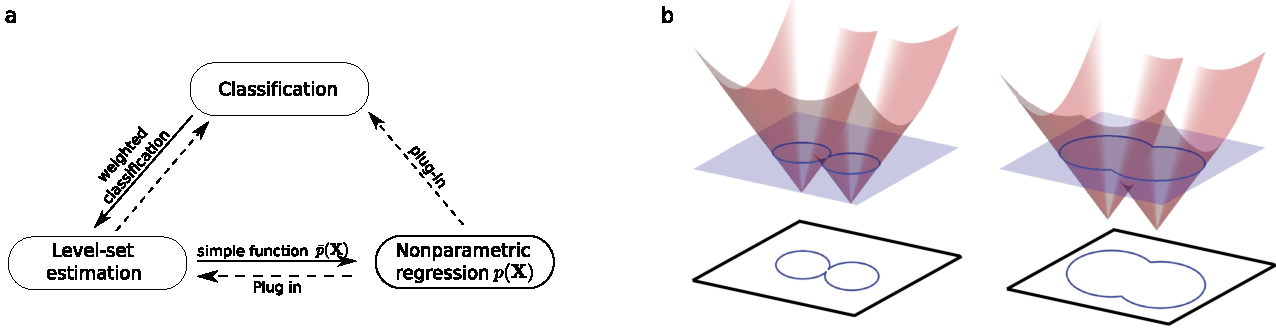
\includegraphics[width=1\textwidth]{level.pdf}
\caption{(a) Our learning reduction approach (solid line) to the three problems of interest. The classical plug-in approaches are depicted in dashed line.  (b) Schematic diagram for nonparametric function estimation via level set aggregations (i.e,\ a series of weighted classifications). Figure (b) is modified from~\cite{gibou2018review}. }\label{fig:diagram}
\end{figure}

\subsection{Related work}
Our work is related to but also clearly distinctive from several lines of existing research. We review some of the main ideas that have emerged. 
 
\subsubsection{Parametric matrix regression}
There has been increased interest in studying matrix-valued predictors for regression; for example, trace regression~\citep{fan2019generalized,hamidi2019low}, network logistic regression~\citep{relion2019network,guha2020bayesian}, and regularized matrix regression~\citep{zhou2014regularized,wang2017generalized}. These methods fall into the broad category of parametric approaches that impose a priori functional form between variables. The most common model in this vein is generalized linear model (GLM) which relates conditional mean to predictors though a known link function. Given a matrix predictor $\mX$ and a response variable $y$, the regression model takes the form
\[
\mathbb{E}(y|\mX)=g(\langle \mB,\mX\rangle), \ \text{with a known function }g(\cdot)\colon \mathbb{R}\to \mathbb{R},
\]
where $\mB$ is an unknown matrix with certain structural constraints depending on the specific problems. The GLM is a popular parametric regression, but nevertheless, this approach lacks the flexibility and often leads to inaccurate prediction in high dimensions. 
 
\subsubsection{Common nonparametric strategies}
A variety of nonparametric regressions have been developed to overcome the limitation of parametric regression. For example, single index models~\citep{hardle1993optimal} extend GLMs by allowing an unknown $g$ in order to provide flexibility in prediction. Nearest neighbor methods~\citep{altman1992introduction} estimate the function by taking the average of responses in the neighbored of predictors. Polynomial regression~\citep{wahba1990spline} and wavelets~\citep{donoho1998minimax} perform curve fitting through basis expansions. Computational efficiency and statistical accuracy are both real concerns as the predictor dimension grows large, in nonparametric regression. Common strategies to mitigate the curse of dimensionality include imposing structural constraints, such as additivity, monotonicity, and/or sparsity, to the regression function.  The nonparametric learning with structural constraints is still very much in development~\citep{geenens2011curse,guntuboyina2018nonparametric}.

Three key challenges have yet to address when we consider matrix-valued predictors. First, matrix-valued predictors encode far richer information than vectors, as mentioned in the earlier brain network example. A naive approach is to transform the predictors into vectors and apply classical nonparametric regression. The practice of vectorization, however, destroys the two-way structural information in the original predictors. 
Second, most nonparametric methods rely on some notion of smoothness in the local neighborhood of predictors. In the context of matrix-valued predictors, however, the predictor space is huge and barely explored by small sample size data. Third, matrix-valued predictors often lead to a high dimensional problem with massive features. The relatively weak assumptions made by nonparametric methods bring new challenges to interpretation. Achieving accurate prediction while maintaining descriptive simplicity will be our goal.


\subsubsection{Nonparametric methods with manifolds} 
Several attempts have been developed to address nonparametric regression with manifold-valued predictors. The manifolds here refer to general nonconventional predictors, such as matrices, tensors, networks, images, and so on. \cite{chen2019nonparametric} extends deep neural network to regression on low-dimensional manifold. \cite{hao2019sparse} develops a sparse additive model with tensor covariates by extending usual spline basis. \cite{zhou2020broadcasted} also considers tensor covariates but instead proposes a broadcasting operation to impose nonlinearity to individual tensor entries. In computer vision, convolution neural network (CNN) has been widely adopted as a nonparametric tool for image data~\citep{goodfellow2016deep}. 
These methods in some sense address the first and part of the second challenge mentioned in the earlier paragraph; they use the conventional wisdom of exploiting low-dimensional structure in the input data in order to achieve accurate prediction. 

Our method share the same ground as theirs, but we provide a completely different paradigm for extracting information from massive high-dimensional data. We develop a low-rank, sparse halfspace learning in the matrix space, and allow the informative features in the matrix-valued predictor to vary from one level to another. Unlike the aforementioned methods, our method relies little on the local neighborhood of predictors but rather on the local neighborhood of responses. More importantly, we do not only tailor a specific nonparametric tool for matrix-valued predictors; we provide a learning paradigm that potentially enables state-of-art classification tools, such as neural network, decision trees, and boosting, to address the more challenge regressing problem. The ability to import and adapt existing classification methods is one advantage of the proposed learning reduction framework.
We also numerically compare our approach with CNN in Section~\ref{sec:simulation}.



\subsubsection{Regression level set estimation}
Level set method has a long history in statistics~\citep{tsybakov1997nonparametric} and computational mathematics~\citep{gibou2018review}. The approach has drawn increased attention because of recent successes in neural network~\citep{atzmon2019controlling}, density estimation~\citep{chen2017density}, classification~\citep{varshney2010classification}, and bandit optimization~\citep{shekhar2019multiscale}. Level sets provide an efficient approach to representing functions. Instead of constructing a function point-wise in the predictor space, the method focuses on the range space (see Figure~\ref{fig:diagram}b). The benefit bears the analogy of Riemann vs.\ Lebesgue integrals in the functional analysis, in the sense that the focus is shifted from domain space to range space. This approach is especially appealing for matrix binary regression, where the feature space is complicated whereas the response is a simple bounded univariate.  
  
Earlier work on level set estimation considers only a single level~\citep{tsybakov1997nonparametric,singh2009adaptive}. Statistical properties for plug-in level set estimates are studied in \cite{audibert2007fast,rigollet2009optimal}. In comparison to our learning reduction, their analysis can be viewed as a \emph{learning induction} approach where the regression function estimates are provided as inputs (Figure~\ref{fig:diagram}a). \cite{wang2008probability} develops a conditional probability estimation method based on support vector machine (SVM), but their results are restricted to fixed number of features (e.g.\ $d=2$ in their example) and vector predictors only. \cite{singh2009adaptive} proposes a partition-based method for multiple level sets extraction, but again their goal is to estimate the level sets per se but not function estimation.  None of these methods address the regression problem or high-dimensional matrix-valued predictors as in our work. 
 
%Most theory takes a reverse question, given an nonparametric regression estimate, how to extract the level sets...  Our provide the theoretical justification to the inverse approach, given multiple level sets approaches, how to recovery the function estimation. This approach may be of independent interest and broader implications beyond the matrix learning tasks. 


 
 
\subsection{Notation and organization} 
Let $\tX\subset \mathbb{R}^{d_1\times d_2}$ be the feature space. Given a function $f\colon \tX \to \mathbb{R}$, we use $\sign f$ to denote its sign function, such that $\sign f(\mX)=1$ if $f(\mX)>0$ and $\sign f(\mX)=-1$ otherwise. The notion of sign function also applies to sets in $\tX$. We use $\sign (\mX\in A)$ to denote the sign function induced by the set $A\subset\tX$, i.e.,\ a function taking value $1$ on the event $\{\mX\in A\}$ and -1 otherwise. We use shorthand $[n]:=\{1,\ldots,n\}$ to denote the $n$-set for $n\in\mathbb{N}_{+}$ and use $|\cdot|$ to denote the cardinality of sets. Let $\newnormSize{}{\cdot}_p$ denote the vector $p$-norm for $p\geq 0$, and $\FnormSize{}{\cdot}$ be the matrix Frobenious norm. Given a $d_1$-by-$d_2$ matrix $\mB$, we use $\mB_i$ to denote the $i$-th row of $\mB$. The $(p,q)$-norm of a matrix $\mB$ is defined as $\newnormSize{}{\mB}_{p,q}=\newnormSize{}{\mb}_q$, where $\mb=(\newnormSize{}{\mB_1}_p,\ldots,\newnormSize{}{\mB_{d_1}}_p)^T\in\mathbb{R}^{d_1}$ consists of the $p$-norms for each of the rows in $\mB$. In particular, $\newnormSize{}{\mB}_{1,0}=|\{i\in [d_1]\colon \mB_i\neq 0\}|$ denotes the number of non-zero rows in $\mB$. An event $E$ is said to occur ``with high probability'' if $\mathbb{P}(E)$ tends to 1 as the matrix dimension $d_{\min}=\min(d_1,d_2)\to\infty$. We denote $a_n\asymp b_n$ if $\lim_n b_n/a_n= c$ for some constant $c>$ and denote $a_n\lesssim b_n$ if $\lim_n b_n/a_n=0.$ We use $\mathds{1}(\cdot)$ to denote the indicator function. 

The rest of the paper is organized as follows. Section~\ref{sec:problem} presents a range of learning tasks, from classification to regression, for matrix-valued predictors. In Section~\ref{sec:idea}, we develop a learning reduction approach by relating the regression to classification, and establish the oracle procedures of nonparamatric matrix regression. In Section~\ref{sec:estimation}, we present the empirical estimation and the associated optimization algorithm. Statistical accuracy, high-dimensional consistency, and excess risk bounds are presented in Section~\ref{sec:theory}. We present the simulations in Section~\ref{sec:simulation} and human connectome Project data analyses in Section~\ref{sec:real}. All technical proofs are deferred to Appendix. 

\section{Review: Three learning problems}\label{sec:problem}

We present the main learning goals of our interest. Let $\mX\in \mathbb{R}^{d_1\times d_2}$ denote the matrix-valued predictor, $y\in\{-1,1\}$ denote the binary label response, and $\mathbb{P}_{\mX,y}$ denote the unknown joint probability distribution over the pair $(\mX,y)$. In the context of binary response, $y$ is a Bernoulli random variable with conditional probability $\mu(\mX)\stackrel{\text{def}}{=}\mathbb{P}(y=1|\mX)$; we generally make no parametric assumptions on the marginal distribution $\mathbb{P}_{\mX}$ or form of $\mu(\mX)$. 


Suppose that we observe a sample of $n$ training data points, $(\mX_1,y_1),\ldots,(\mX_n,y_n)$, identically and independently distributed (i.i.d.) according to $\mathbb{P}_{\mX,y}$. Let $(\mX_{\text{new}},y_{\text{new}})$ be a future unseen test point drawn independently from the same distribution. Our goal is to predict $y_{\text{new}}$ based on $\mX_{\text{new}}$. We often omit the subscript ``new'' and simply write $(\mX,y)$ for the prototypical test point. The relevant probabilistic statements should be interpreted as taken jointly with respect to $(\mX,y)$.

We consider three learning problems: classification, level set estimation, and regression. 

\begin{enumerate}[label={2.\arabic*},wide, labelwidth=!, labelindent=0pt]
\item {\it Classification}: Classification is the problem of predicting the label $y\in \{-1,1\}$ to which the new matrix $\mX$ belongs. A prediction rule (also called a classifier) decides that $y=1$ if $\mX\in S$ and $y=-1$ if $\mX \not\in S$, where $S$ is a Borel subset of $\tX$. We formulate the classification problem as choosing a classifier $S\in \tS$, from a given set of candidate classifiers $\tS$, that minimizes the expected classification error 
\begin{equation}\label{eq:classloss}
R(S)=\mathbb{P}_{\mX,y}\left[y\neq \sign(\mX\in S)\right].
\end{equation}
The $R(S)$ is also called the classification risk. When the candidate set $\tS$ consists of all Borel subsets of $\tX$, the minimizer of~\eqref{eq:classloss} is called the Bayes classifier. It is known that the Bayes classifier can be written as 
\begin{equation}\label{eq:bayes}
\bayesS(1/2)=\{\mX\in \tX \colon \mu(\mX)\geq 1/2\}.
\end{equation}
Note that the minimizer of~\eqref{eq:classloss} is non-unique, because arbitrary prediction rules are allowed on the boundaries $\partial S_{\text{bayes}}(1/2) = \{\mX\in \tX\colon \mu(\mX)=1/2\}$. Without loss of generality, we will use~\eqref{eq:bayes} as the canonical form of the Bayes classifier. 

In practice the population distribution is unknown, so the objective function~\eqref{eq:classloss} and the minimizer needs to be estimated through the data $(\mX_i,y_i)_{i=1}^n$. Our first goal is to estimate the Bayes classifier for matrix classification. 

{\bf Question 1.} How to perform classification when matrix dimension far exceeds the sample size $n$?

\item {\it Level set estimation}: The problem of level set estimation generalizes the classification task. For a given $\pi\in(0, 1)$, the target $\pi$-level set of the conditional probability function $\mu(\mX)$ is defined as
\begin{equation}\label{eq:level}
\bayesS(\pi) = \{\mX\in\tX \colon \mu(\mX)\geq \pi\}.
\end{equation}
An important fact is that the set $\bayesS(\pi)$ optimizes the weighted classification risk~\citep{willett2007minimax,scott2007regression,wang2008probability}. Specifically, among all Borel subsets of $\tX$, the set $S_{\text{bayes}}(\pi)$ is the global minimizer of the expected $\pi$-weighted classification error,
\begin{equation}\label{eq:risklevel}
R_\pi(S)=\mathbb{E}\left[ w_{\pi}(y)\mathds{1}(y\neq \sign(\mX\in S))\right],
\end{equation}
where $y\in\{-1,1\}$ is distributed based on $\mathbb{P}(y=1|\mX)=\mu(\mX)$, and we define $w_{\pi}(y)=1-\pi$ or $\pi$ depending on $y=1$ or $-1$; that is, $w_\pi(\cdot)$ assigns unequal weights to the two labels. In light of~\eqref{eq:classloss} and~\eqref{eq:risklevel}, the level set problem extends the usual classification from equal weight $\pi=1/2$ to general weight $\pi \in(0,1)$. %Accurate level set estimation plays an important role in applications of geographical elevation maps, imaging contour detection, and motion tracking. 
We consider the following question:

{\bf Question 2.} How to simultaneously estimate the level set and identify important features in the matrix-valued predictors, for the goal of interpretable prediction?


\item {\it Nonparametric binary regression}: The problem of nonparametric regression is to estimate the conditional mean $\mathbb{E}(y|\mX)$ as a multivariable function in the predictor space. In our contexts, the nonparametric regression is equivalent to estimating the conditional probability $\mu(\mX)=\mathbb{P}(y=1|\mX)=\frac{1}{2}(\mathbb{E}(y|\mX)+1)$. Throughout the paper we will focus on $\mu(\mX)$ and refer to it as the regression function. 
The function $\mu(\mX)$, is the global minimizer, among all measurable functions $f\colon \tX\to[0,1]$, of the expected squared error,
\begin{equation}\label{eq:regression}
R_{\text{reg}}(f)=\mathbb{E}\left[{1\over 2}(y+1)-f(\mX)\right]^2,
\end{equation}
where $R_{\text{reg}}(f)$ is also known as regression risk. Our final goal is the function estimation:

{\bf Question 3.} How to learn the binary regression function $\mu(\mX)$ in the high-dimensional matrix space?
\end{enumerate}


The three problems of our interest represent a range of learning tasks with increasing difficulties. Classification is a special case of level set estimation with $\pi=1/2$, whereas the level set is a discrete approximation of the regression function. A common approach is to address regression first, and then solve the earlier two using plug-in estimates (Figure~\ref{fig:diagram}a). This procedure, however, undermines the fact that regression is generally harder than the other two. Indeed, as we show in Section~\ref{sec:theory}, regression has a slower convergence rate $\tO(n^{-1/2})$ compared to the rate $\tO(n^{-1})$ of classification. Ignorance of the increased complexity violates Vapnik’s maxim: \emph{When solving a given problem, one should try to avoid solving a more general problem as an intermediate step.} 

\begin{figure}
\centering
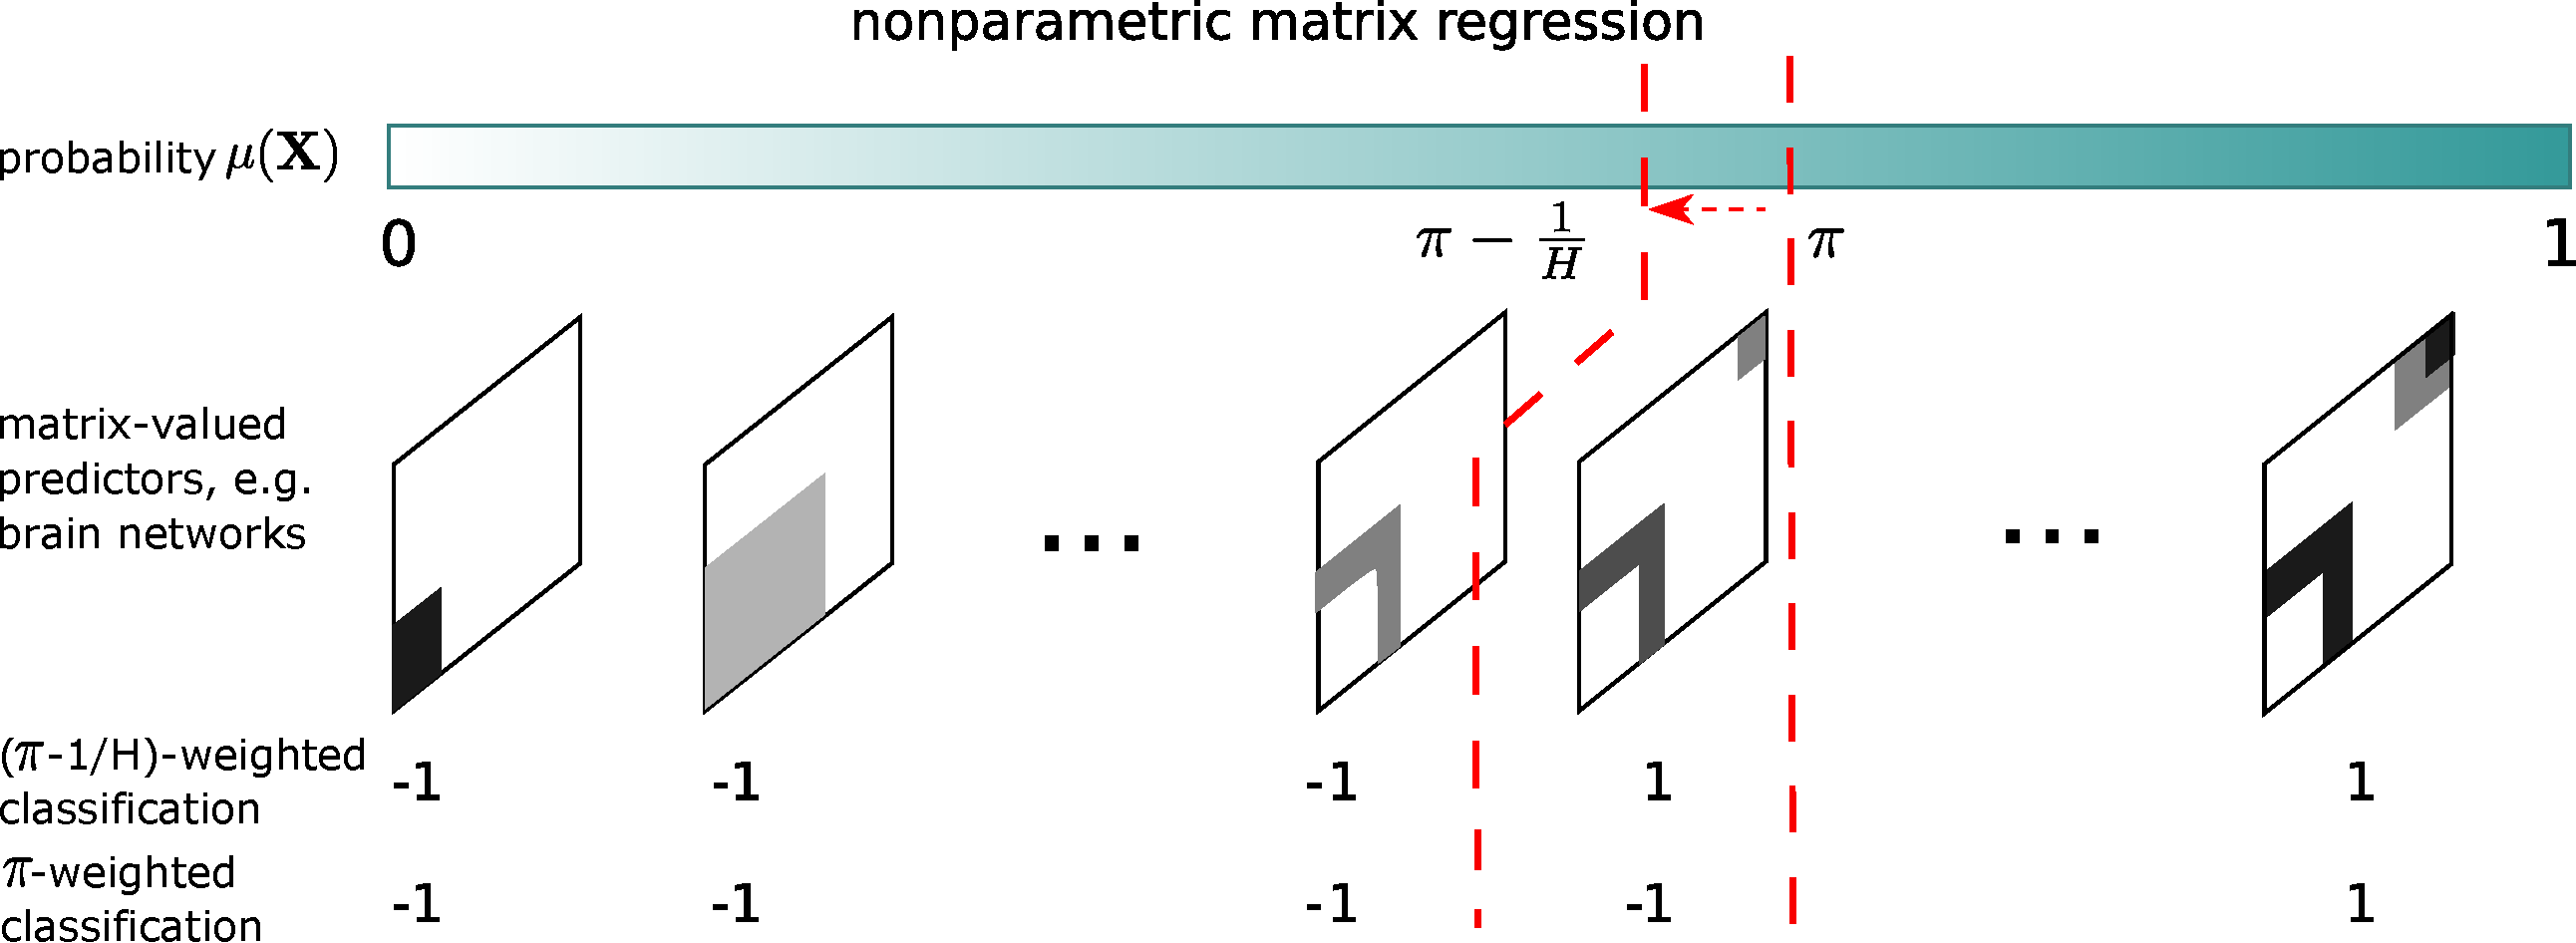
\includegraphics[width=15cm]{demo_method2.pdf}
\caption{Level-set approaches to matrix binary nonparametric regression. We use weighted classification to find the level-set in the matrix space, and then estimate the target regression function via aggregation. }\label{fig:method}
\end{figure}

\section{From classification to regression: a new deal}\label{sec:idea}
We develop a ``learning reduction'' approach (Figure~\ref{fig:diagram}a) by relating the regression to classification. The latter problem is more fundamental and statistically easier to address. In general, regression requires more assumptions than classification. Our learning reduction approach bridges these two tasks using level set estimation, a problem lies somewhere in between. The connection allows us to disentangle complexity and leverage existing algorithms. 

In this section we describe the oracle procedure of estimating regression function $\mu(\mX)$ when the true distribution $\mathbb{P}_{\mX,y}$ is known. This simplified situation leads to a cleaner characterization with deterministic risk functions in~\eqref{eq:classloss}, \eqref{eq:risklevel}, and \eqref{eq:regression}. The finite sample estimation will be presented in Section~\ref{sec:estimation}, in which we address the general case with unknown distribution $\mathbb{P}_{\mX,y}$, and all the information is based on empirical (stochastic) risk estimated from the training set $(\mX_i,y_i)_{i=1}^n$. 


\subsection{Level set approaches to nonparametric binary regression}\label{sec:bridge}
Figure~\ref{fig:method} illustrates the main idea of our approaches. We use a series of weighted classifications to find the level sets in the matrix space, and then estimate the regression function $\mu(\mX)={1\over 2}(\mathbb{E}(y|\mX)+1)$ via level set aggregation. Our building block is to use level sets to estimate regression function $p(\cdot)$ through classifications. The level set approach bridges the two sides of a same coin -- characteristic (set indicator) functions in functional analysis and weighted classifications in statistical learning. 

Specifically, let $\mu(\cdot)\colon \tX \to [0,1]$ be the target regression function of interest, and $\bayesS(\pi)=\{\mX\in \tX\colon \mu(\mX)\geq \pi\}$ be the associated $\pi$-level set. Let $\Pi=\{{1\over H}, {2\over H}, \ldots, {H-1\over H} \}$ be a sequence of evenly spaced points in $[0,1]$, where $H\in\mathbb{N}_{+}$ is the resolution parameter. We introduce an $H$-step function $\bar \mu(\cdot)\colon \tX \to [0,1]$ by
\begin{equation}\label{eq:stepfunction}
\bar \mu(\mX)= {1\over 2H}  \sum_{\pi \in \Pi} \sign (\mX\in \bar S(\pi))+{1\over 2}, \quad \text{for all }\mX\in\tX\subset \mathbb{R}^{d_1\times d_2},
\end{equation}
where, for every $\pi\in\Pi$, the set $\bar S(\pi)\subset \tX$ is the classifier that minimizes the $\pi$-weighted classification risk,
\begin{equation}\label{eq:constrained}
\bar S(\pi) \stackrel{\text{def}}{=} \argmin_{S\in \tS}R_\pi(S), \quad \text{where}\quad R_\pi(S)=\mathbb{E}\left[ w_{\pi}(y)\mathds{1}(y\neq \sign (\mX\in S))\right],
\end{equation}
subject to the constraint $S\in\tS$, with $\tS$ being a given candidate set of classifiers in $\tX$. When the set $\tS$ is rich enough, e.g., $\tS$ consists of all Borel subsets of $\tX$, then $\bar S(\pi)$ has the same risk as $\bayesS(\pi)$. We leave the $\tS$ in general here; the specific choice of $\tS$ will be described in Section~\ref{subsec:linear class}. 

In order to address the accuracy between $\bar \mu(\mX)$ and $\mu(\mX)$, we establish the recovery guarantee of level sets $S(\pi)$ from optimization~\eqref{eq:constrained}. The Bayes classifier $\bayesS(\pi)$ minimizes the weighted classification risk $R_\pi(S)$; the inverse, however, may not be true because of possible multiple global minimizers of $R_\pi(S)$. The uniqueness and stability around $\bayesS(\pi)$ turns out to play a key role in the accurate estimation of $\mu(\mX)$. 

We introduce the following notion to characterize the behavior of the regression function near the level set boundaries $\partial S_{\text{bayes}}(\pi) = \{ \mu(\mX)= \pi\}$. The condition essentially quantifies the uniqueness of level sets recovery from weighted classification.

Some additional notation is needed. We call a level $\pi\in[0,1]$ a mass point if the level set boundary $\partial \bayesS(\pi)$ has non-zero measures under $\mathbb{P}_{\mX}$. Let $\tN=\{\pi\in[0,1] \colon \mathbb{P}_{\mX}\left[\mu(\mX)=\pi\right]\neq 0\}$ denote the collection of mass points in $\mu(\mX)$. Assume $|\tN|\leq c<\infty$ for some constant $c>0$. 

\begin{defn} [$\alpha$-regularity]\label{ass:decboundary} Fix $\pi \notin \tN$. A function $\mu(\mX)$ is called $(\alpha,\pi)$-locally regular, if there exist constants $C=C(\pi)>0, \alpha=\alpha(\pi)\in[0,1]$, such that,
\begin{equation}\label{eq:mass}
\sup_{0\leq t<\rho(\pi, \tN)}{\mathbb{P}_{\mX}(|\mu(\mX)-\pi|\leq t)\over t^{\alpha/(1-\alpha)}}\leq C,
\end{equation}
where $\rho(\pi,\tN)\stackrel{\text{def}}{=}\min_{\pi'\in \tN} |\pi-\pi'|$ denotes the distance from $\pi$ to the nearest point in $\tN$.  When $\tN = \phi$, we define $\rho(\pi,\tN)=1$. The largest possible $\alpha=\alpha(\pi)$ is called the smoothness index at level $\pi$. In particular $\alpha=1$ means the numerator in~\eqref{eq:mass} is zero. 

If $\mu(\mX)$ is $(\alpha,\pi)$-locally regular for all $\pi \in [0,1]$ except for a finite number of points, and $C=\max_{\pi} C(\pi)<\infty$, then we call $\mu(\mX)$ is $\alpha$-globally regular. 
\end{defn}

The global regularity controls the uniform behavior of $\mu(\mX)$ over all possible $\pi$'s (except for a finite number of points). The exponent $\alpha$ quantifies the concentration of probability mass $\mu(\mX)$ around level set boundaries. We show that the global regularity implies the identifiability of $\bayesS(\pi)$ from optimization \eqref{eq:constrained} for almost all $\pi$'s. For two sets $S_1, S_2 \in \mathbb{R}^{d_1\times d_2}$, we define the probabilistic set difference 
\begin{align}\label{eq:riskdiff}
d_{\Delta}(S_1,S_2)\stackrel{\text{def}}{=}\mathbb{P}_{\mX}(S_1\Delta S_2)=\mathbb{P}_{\mX}\{\mX\colon \mX\in S_1\setminus S_2 \text{ or }S_2\setminus S_1\},
\end{align}
and the excess classification risk
\begin{align}\label{eq:setdiff}
d_\pi(S_1,S_2)\stackrel{\text{def}}{=} R_{\pi}(S_1)-R_{\pi}(S_2).
\end{align}

\begin{prop}[Identifiability]~\label{thm:identifiability} Suppose the regression function $\mu(\mX)$ is $\alpha$-globally regular with $\alpha\in[0,1]$. Then, 
\begin{align}\label{eq:identity}
d_{\Delta}(S,\bayesS(\pi)) \lesssim d_\pi^\alpha(S,\bayesS(\pi))+{1\over\rho(\pi, \tN)} d_\pi(S,\bayesS(\pi)),
\end{align}
for all sets $S\in\mathbb{R}^{d_1\times d_2}$ and all levels $\pi\in[0,1]$ except for a finite number of points. 
\end{prop}

The bound~\eqref{eq:identity} controls the worst-case perturbation of classifiers in the probability space $\mathbb{P}_{\mX}$ with respect to weighted classification risks. When $\alpha\neq 0$, the inequality~\eqref{eq:identity} immediately implies the uniqueness of $\bayesS(\pi)$ up to a measure-zero set in $\mathbb{P}_{\mX}$, whereas $\alpha=0$ corresponds to no identifiability.  Notice that $\rho(\pi,\tN)$ becomes a constant for fixed $\pi$, implying that local regularity ensures the identifiability of Bayes set $\bayesS(\pi)$.


Our identifiability characterization generalizes the earlier results for single level set estimation~\citep{singh2009adaptive,xu2020class}. Inspection of the proof shows that the set estimation is more difficult at levels where the point mass concentrates (small $\alpha$), as intuition would suggest. Consider a simple case when the entries of matrix $\mX$ are i.i.d.\ drawn from $\text{Uniform}[-1,1]$; that is, $\mathbb{P}_{\mX}$ is the Lebesque measure on $[0,1]^{d_1d_2}$. Then, the best rate $\alpha\to 1$ corresponds to a clear separation with no point mass at the boundary, whereas the worst rate $\alpha\to 0$ corresponds to a heavy mass of $\mu(\mX)$ near the boundary. A typical intermediate case is $\alpha=1/2$ when $\mu(\mX)$ is a locally bilipschitz function (see Proposition~\ref{prop:polynomial} in Appendix).

Now we reach the main result of this section by putting together the proposal~\eqref{eq:stepfunction},~\eqref{eq:constrained} and Proposition~\ref{thm:identifiability}. Define the regression excess risk by $R_{\textup{reg}}(\bar \mu) - R_{\textup{reg}}(\mu)$.
The following result bounds the regression excess risk using classification excess risk.

\begin{thm}[Nonparametric regression via weighted classifications]\label{thm:twobounds} Suppose that the regression function $\mu(\mX)$ is $\alpha$-globally regular with $\alpha\in[0,1]$. Let $\bar \mu(\mX)$ the step function~\eqref{eq:stepfunction} constructed from weighted classifiers. Then, the regression excess risk is bounded by the classification excess risk; i.e.,
\begin{align}\label{eq:approximation}
R_{\textup{reg}}(\bar \mu) - R_{\textup{reg}}(\mu)&\leq 4\mathbb{E}_{\mX}\left|  \mu(\mX)-\bar \mu(\mX)\right|\notag\\
&\lesssim {1\over H}+ \frac{1}{H}\sum_{\pi\in\Pi\setminus\tN}\left\{d_\pi^{\alpha}(\bayesS(\pi),\bar S(\pi))+ {1\over\rho(\pi, \tN)} d_\pi(\bayesS(\pi),\bar S(\pi))\right\},
\end{align}
for all resolution parameter $H=|\Pi|\in \mathbb{N}_{+}$. 

\end{thm}

Theorem~\ref{thm:twobounds} shows the key role of $\bar \mu(\mX)$ in bridging regression and classification. The results suggest that the estimation of $\mu(\mX)$ can be reduced to estimation of $\bar \mu(\mX)$, or equivalently, to a series of weighted classifications $(\bar S(\pi))_{\pi\in\Pi}$. The regression excess risk bound~\eqref{eq:approximation} has two terms. The first term is the bias due to the step function approximation to the regression function. The second term is the classification excess risk of recovering $\bayesS(\pi)$ from optimization~\eqref{eq:constrained}. In the case of unknown population distribution $\mathbb{P}_{\mX,y}$, the second term should be plugged in using the empirical risk, which results in a variance-bias error due to finite sample size (see Section~\ref{sec:estimation}). 

Estimating $\bar \mu(\mX)$ as a surrogate of $\mu(\mX)$ provides several benefits. From a computational perspective, $\bar \mu(\mX)$ is a finite combination of weighted classifiers, which are easier to solve than a direct regression. From the statistical perspective, the function $\bar \mu(\mX)$ provides a valid approximation to $\mu(\mX)$ even when $\mu(\mX)$ is non-regular and irregular. In particular, the estimation accuracy relies little on the local neighborhood of $\mX$ but rather on the local neighborhood of $\mu(\mX)$. Note that the former is a $d_1d_2$-dimensional random variable whereas the later is a $[0,1]$-valued univariate random variable. The shifted focus of local structure to the range space is especially appealing for matrix-valued predictors, since the predictor space is high dimensional and often barely explored by small sample size data.  

\subsection{Sparse and low-rank function boundaries}\label{subsec:linear class}
We describe the choice of candidate sets $\tS$ in~\eqref{eq:constrained}. A desirable $\tS$ should balance the prediction and interpretability; i.e., $\tS$ should be flexible enough for accurate prediction while being simple enough for high interpretability. We propose to optimize~\eqref{eq:constrained} over the family of linear halfspaces; i.e.,
%rewrite the optimization~\eqref{eq:constrained} as the minimization over continuous-valued functions,
\begin{equation}\label{eq:optimization}
\bar S(\pi) = \{\mX\colon\bar f(\mX)\geq 0\},\quad  \text{with}\quad  \bar f(\mX)= \argmin_{f(r,s_1,s_2)\in\tF}\mathbb{E}\left[w_\pi(y)\mathds{1}(y\neq \sign f(\mX))\right],
\end{equation}
%where $\bar f\in\tF$ is a continuous-valued function from $\mathbb{R}^{d_1\times d_2}$, and its sign induces the classifier $\bar S(\pi)\in\tS$. The choice of $\tS$ thus reduces to the choice of function family $\tF$. A desirable $\tF$ should balance the prediction and interpretability; i.e., $\tF$ should be flexible enough for accurate prediction while being simple enough for high interpretability. We propose the linear function family 
where the function family $\tF(r,s_1,s_2)$ consists of linear classifiers with low-rank two-way sparse matrix coefficients,
\begin{align}\label{eq:class}
\tF(r,s_1,s_2)=\{f\colon \mX\mapsto \langle \mX, \mB \rangle +b \ \big|\ \text{rank}(\mB)\leq r, \ \text{supp}(\mB)\leq (s_1,s_2), \ \mB\in\mathbb{R}^{d_1\times d_2},\ b\in\mathbb{R}\}.
\end{align}
Here $\text{rank}(\mB)$ denotes the rank of the coefficient matrix, and $\text{supp}(\mB)$ denotes the two-way sparsity parameter with $s_1=\newnormSize{}{\mB}_{1,0}$ and $s_2=\newnormSize{}{\mB^T}_{1,0}$ being the numbers of non-zero rows and columns of $\mB$, respectively. For the theory, we assume that $(r,s_1,s_2)$ are known; the adaptation to unknown $(r, s_1, s_2)$ in practice is described in Section~\ref{sec:simulation}.  
Combining formulations~\eqref{eq:stepfunction},~\eqref{eq:optimization} and~\eqref{eq:class} yields our (oracle procedure of ) ``learning reduction'' approach to nonparametric matrix regression.


The low-rank two-way sparse classifier~\eqref{eq:class} enables efficient variable selection in high-dimensional matrices, thereby achieving high interpretability in prediction. In the brain network analysis, scientists are interested in identifying important nodes attached to at least one active edges with non-zero effects. Classical entrywise sparsity essentially treats $\mX$ as ``a bag of non-ordered edges'', and loses the two-way paring information among entries. In contrast, our two-way sparsity efficiently identifies the underlying active nodes by making use of matrix structure in the predictors. 

It is worthy noting that the linearity in the classifiers $\tF$ does not preclude the global nonlinearity in the regression function $\mu(\mX)$ or its variant $\bar \mu(\mX)$. As shown in the following examples, many nonlinear regression functions in existing literature are special cases of our representation~\eqref{eq:optimization} with~\eqref{eq:class}, in the sense that their level sets are precisely halfspaces. 

\begin{example}[Monotonic single index models~\citep{alquier2013sparse,ganti2017learning}]\label{example:1}
Suppose the true regression function can be expressed as $\mu(\mX)= g(\langle \mX,\mB\rangle)$, where $g(\cdot)\colon \mathbb{R}\to [0,1]$ is an arbitrary monotonic link function, and $\mB$ is a low-rank two-way sparse matrix. Then, for every $\pi\in(0,1)$, there exists $f_\pi\in \tF(r,s_1,s_2)$, such that $\sign(\mu(\mX)-\pi)= \sign f_\pi(\mX)$. Our method generalizes nonlinear single index model to high dimensional matrices by joint learning matrix coefficient $\mB$ and nonlinear function $g$. 
\end{example}

Single index models with (unknown) monotonic links, such as logistic function $g(z)=(1+\exp(-z))^{-1}$, arctangent function $g(z)={1\over \pi}\arctan(z)+{1\over 2}$, truncated rectified linear unit (ReLU) function $g(z)=z\mathds{1}(z\in[0,1])+\mathds{1}(z>1)$, and any arbitrary inverse cumulative distribution functions (CDF) are included in our classifier functions. In particular, our model extends parametric matrix regression with known link functions~\citep{zhou2014regularized,guha2020bayesian,relion2019network} to the nonparametric regression with unknown link functions. 

There are usually two approaches for analyzing association between matrix data and binary labels. One approach is to analyze the conditional distribution $y|\mX$ from the prospective model. The other approach is to analyze the conditional distribution $\mX|y$ from the retrospective model. Although our proposal is built on the former, our classifier function also incorporates the retrospective models from matrix linear discriminant analysis (LDA)~\citep{hu2020matrix}. 
\begin{example}[Multivariate normal mixtures]\label{example2}Suppose the matrix-valued predictor $\mX$ follows a Gaussian mixture distribution, $\mX|\{y=-1\}=\mB_1+\mE_1$ and $ \mX|\{y=1\}=\mB_2+\mE_2$, where $(\mB_1-\mB_2)$ is a low-rank two-way sparse matrix, and $\mE_1, \mE_2$ are two mutually independent noise matrices with i.i.d.\ $N(0,1)$ entries. Then, for every $\pi\in(0,1)$, $\sign(\mu(\mX)-\pi)= \sign f_\pi (\mX)$ for some $f_\pi \in \tF(r,s_1,s_2)$. 
\end{example}

More generally, we have established the characterization by extending two classes of $\mX$ to a series of $\mX=\mX(\pi)$ over a continuous spectrum of $\pi \in (0,1)$ (see Appendix~\ref{sec:joint}). Our level-set approach essentially learns the right ``sorting'' of $\mX(\pi)$ against the index $\pi\in(0,1)$ (see Figure~\ref{fig:method}), thereby facilitating the estimation of relationship $\pi=\pi(\mX)$. 

%The following proposition gives a sufficient condition for exact recovery of level sets through halfspaces; the results show that what essentially matters is the boundary of level sets.  
%where $S(\pi)$ be the level set defined in~\eqref{eq:level} and $\bar S(\pi)$ be the classifier defined in~\eqref{eq:optimization} optimized over $\tF(r,s_1,s_2)$. 

%\begin{prop} Let $\mu(\mX)$ be a regression function whose level sets are characterized by linear classifiers in $\tF(r,s_1,s_2)$; that is, for every $\pi\in (0,1)$, there exists $f_\pi\in\tF(r,s_1,s_2)$ such that $\sign (\mu(\mX)-\pi)=\sign (f_\pi)$. Then, $\mu(\mX)$ admits the single-index model; i.e., there exists a monotonic function $g\colon \mathbb{R}\to (0,1)$ and a low-rank two-way sparse matrix $\mB$ such that $\mu(\mX)=g(\langle \mX, \mB \rangle)$ for all $\mX\in\mathbb{R}^{d_1\times d_2}$.
%\end{prop}

%\begin{prop}[Low-rank and sparse boundaries]\label{prop:px} Let $\mu(\mX)$ be a regression function continuous in $\mX\in\mathbb{R}^{d_1\times d_2}$. Suppose that there exists a low-rank two-way sparse matrix $\mB_\pi$ and a real value $b_\pi\in\mathbb{R}$, such that the boundary set $\partial S(\pi)=\{\mX\colon \mu(\mX)=\pi\}$ is included in the set $\{\mX\colon \langle \mX, \mB_\pi \rangle = b_\pi\}$. Then $\sign (\mu(\mX)-\pi)=\sign (f_\pi(\mX))$ for some $f_\pi(\mX)\in \tF(r,s_1,s_2)$. Note that $(\mB_\pi, b_\pi)$ is allowed to vary depending on $\pi$. 
%\end{prop}

In principle, more complicated classifiers, such as neural network, decision trees, and boosting, can also be brought to bear on the level set construction~\eqref{eq:optimization}. The ability to import and adapt existing classification methods is one advantage of the proposed learning reduction framework. We find that, in our motivating brain network analysis, the low-rank two-way sparse classifiers~\eqref{eq:class} are able to provide the benefit of interpretable predictions with high accuracy (see Section~\ref{sec:real}). 

\section{Estimation}\label{sec:estimation}
In previous sections we have established the oracle procedure from classification to regression (Figure~\ref{fig:method}). In this section we address the empirical learning problems when the true distribution $\mathbb{P}_{\mX,y}$ is unknown. The objective function in the earlier optimization now becomes empirical (stochastic) risks calculated from high dimensional training data $(\mX_i,y_i)_{i=1}^n$. 

\subsection{Large-margin learning with high dimensional matrices}
When the distribution $\mathbb{P}_{\mX,y}$ is unknown, we propose the regression function estimate $\hat \mu(\cdot)\colon \tX \to [0,1]$ by
\begin{equation}\label{eq:stepfunctionsample}
\hat \mu(\mX)= {1\over 2H}  \sum_{\pi \in \Pi} \sign (\mX\in \hat S(\pi))+{1\over 2},\quad \text{for all }\mX\in\tX\subset\mathbb{R}^{d_1\times d_2}.
\end{equation}
Here, for every $\pi\in\Pi$, the set $\hat S(\pi)\subset \tX$ is the estimated classifier from empirical surrogate risk minimization,
\begin{align}\label{eq:large-margin}
\hat S(\pi) = \{\mX \colon \hat f_\pi(\mX) \geq 0\}, \quad \text{with}\quad \hat f_\pi=\min_{f\in\tF(r,s_1,s_2)}\left\{ {1\over n}\sum_{i=1}^n w_{\pi}(y_i)\ell\left(y_if(\mX_i)\right)+ \lambda \FnormSize{}{f}^2\right\},
\end{align}
where $w_\pi(y) = 1-\pi $ if $y = 1$ and $w_\pi(y)=\pi$ if $y = -1$ is the label-dependent weight; $\ell(z)\colon \mathbb{R}\mapsto \mathbb{R}_{\geq 0}$ is the surrogate classification loss defined as a function of margin $z=yf(\mX)$; $\lambda>0$ is the penalty parameter; and we define the penalization term $\FnormSize{}{f}=\FnormSize{}{\mB}$, with $\mB$ being the coefficient matrix associated with $f\in\tF(r,s_1,s_2)$. Examples of large-margin loss functions are hinge loss $\ell(z) = (1-z)_+$ for support vector machines, logistic loss $\ell(z) =\log(1+e^{-z})$ for important vector machines, and $\psi$-loss $\ell(z)=2\min(1,(1-z)_+)$ with $z_{+}=\max(z,0)$. Our algorithm implements the hinge loss for illustration, although our framework and theory are applicable to general large-margin losses~\citep{bartlett2006convexity}. 

The estimation~\eqref{eq:large-margin} generalizes the oracle formulation~\eqref{eq:optimization} from three aspects. First, the population expectation in~\eqref{eq:optimization} is replaced by the empirical sample average, which is common in statistical learning problems with i.i.d.\ assumption. Second, we add the ridge penalization $\lambda\FnormSize{}{f}^2$ to control the magnitude of the classifiers. The tuning parameter $\lambda$ depends on the sample size and the problem dimension as we will describe in Section~\ref{sec:theory}. The resulting sieve estimate enjoys numerical stability and statistical accuracy. In practice, we choose $\lambda$ in a data-adaptive fashion via cross validation. Third, we replace the binary loss in~\eqref{eq:optimization} by a more manageable large-margin loss. This relaxation allows us to leverage efficient large-margin algorithms while maintaining desirable statistical performance under mild assumptions. 


\subsection{Alternating optimization for structural risk minimization}
We describe the optimization algorithm for solving matrix classification and regression. We focus on the general $\pi$-weighted classification~\eqref{eq:large-margin} because both classification and regression naturally follow by setting $\pi={1\over 2}$, and $\pi\in\{{1\over H},\ldots,{1-H\over H}\}$, respectively. For brevity, we present the algorithm assuming zero intercept in the classifier functions~\eqref{eq:class}, and use $\tF(r,s_1,s_2)$ to denote the set of matrices satisfying $\text{rank}(\mB)\leq r$ and $\text{supp}(\mB)\leq (s_1,s_2)$. The estimation problem~\eqref{eq:large-margin} is formulated as an optimization over matrices,
\begin{equation}\label{eq:sampleoptim}
\min_{\mB \in \tF(r,s_1,s_2)}L(\mB),\quad \text{where }L(\mB)={1\over n}\sum_{i=1}^nw_\pi(y_i)\ell(y_i\langle \mX_i,\mB \rangle) + \lambda\FnormSize{}{\mB}^2,
\end{equation}
where the objective function can be either convex (such as hinge loss, logistic loss) or non-convex ($\psi$-loss). The optimization~\eqref{eq:sampleoptim} has a non-convex feasible region because of the low-rank and sparse constraint. 

We propose an alternating direction method of multipliers (ADMM) approach to solve problem of this type. ADMM introduces a dual variable and an additional feasibility constraint to perform coordinate descent in the corresponding augmented Lagrangian function. The augmented ADMM objective in our context is given by
\begin{equation}\label{eq:ADMM}
L(\mB,\mS,\mLambda,\rho)={1\over n}\sum_{i=1}^nw_\pi(y_i)\ell(y_i\langle \mX_i,\mB \rangle) + \lambda\FnormSize{}{\mB}^2+\rho\FnormSize{}{\mB-\mS}^2+\langle \mLambda, \mB-\mS\rangle,
\end{equation}
and $\mB\in \mathbb{R}^{d_1\times d_2}$ is the unconstrained primal variable, $\mS\in\tF(r,s_1,s_2)$ is the constrained dual variable, $\mLambda\in\mathbb{R}^{d_1\times d_2}$ is the  Lagrangian multiplier, and $\rho>0$ is the step-size parameter. Note that formulation~\eqref{eq:ADMM} has moved the non-convexity from the first two terms in $\mB$ to the last two simpler terms in $\mS$. This separability of ADMM makes the optimization efficient for a wide range of loss functions and constraints. 

We optimize the ADMM objective~\eqref{eq:ADMM} via coordinate descent, by iteratively update one variable at a time while holding others fixed. Each update in the ADMM reduces to a simpler problem and can be efficiently solved by standard algorithms. Specifically, given variables $(\mS,\mLambda,\rho)$ and $\bar \mS\stackrel{\text{def}}{=}{1\over 2(\rho+\lambda)}(2\rho\mS-\mLambda)$, the objective with respect to $\mB$ is
\begin{align}\label{eq:primal}
L(\mB|\mS,\mLambda,\rho)={1\over n}\sum_{i=1}^n w_\pi(y_i)\ell(y_i\langle\mX_i,\mB\rangle)+(\lambda+\rho)\FnormSize{}{\mB-\bar \mS}^2.
\end{align}
This unconstrained optimization is a usual vector-based classification with ridge penalty and an offset $\bar \mS$. Therefore, various loss functions and fast software can be adopted into~\eqref{eq:primal} such as weighted SVM, logistic, and $\psi$-learning. Similarly, given $(\mB,\mLambda,\rho)$ and $\bar \mB\stackrel{\text{def}}{=}{1\over 2\rho}(2\rho\mB+\mLambda)$, the objective with respect to $\mS$ is
\begin{equation}\label{eq:dual}
L(\mS|\mB,\mLambda,\rho)=\FnormSize{}{\mS-\bar \mB}^2,\quad \text{subject to }\mS\in\tF(r,s_1,s_2).
\end{equation}
This formulation is equivalent to the best sparse and low rank approximation, in the least-square sense, to the matrix $\mB$. Compared to the original objective~\eqref{eq:sampleoptim}, the F-norm based objective makes the optimization easier to handle. A number of algorithms have been designated to approximately solve this problem, including sparse PCA, sparse SVD, and projection pursuit. We use the recently-developed double projection algorithm for~\eqref{eq:dual} which has provably better performance than convex alternatives in high dimensional regimes~\citep{yang2016rate}. Finally, the Lagrangian multiplier $\mLambda$ is updated by standard scheme $\mLambda\leftarrow\mLambda+2\rho(\mB-\mS)$.  These steps are performed until the algorithm convergence within tolerance. The value $\rho$ controls the closeness between dual and primal variables. We initialize $\rho$ from 0.1 and increases its value geometrically throughout iterations. In practice, we observed this scheme gives a good balance between the variable feasibility and convergence speed, although other self-tuning methods are also possible~\citep{parikh2014proximal}. Algorithm \ref{alg:weighted} gives the full description for the $\pi$-classification. 

 \begin{algorithm}[ht]
  \caption{{\bf Matrix classification and level-set estimation via ADMM} } \label{alg:weighted}
\KwIn{Data $\{ (\mX_i,y_i)\in \mathbb{R}^{d_1\times d_2}\times \{-1,1\}\colon i\in[n]\}$, rank $r$, support $(s_1,s_2)$, ridge parameter $\lambda$, a target level $\pi \in (0,1)$.}
\KwOut{Estimated $\pi$-level set $\hat S(\pi) = \{\mX\in\mathbb{R}^{d_1\times d_2}\colon \hat f(\mX)\geq 0\}$.}
{\bf Initialize:} primal variable $\mB$, dual variable $\mS$, Lagrangian multiplier $\mLambda=\mathbf{0}$, step size $\rho=0.1$.\\[.1cm]
{\bf Do until converges}\\[.1cm]
\hspace*{.2cm}{\bf Update} $\mB$ fixing $(\mS,\mLambda,\rho)$: 
$\mB \leftarrow \argmin_{\mB} L(\mB|\mS,\mLambda,\rho)$, where $L(\mB|\mS,\mLambda,\rho)={1\over n}\sum_{i=1}^n w_\pi(y_i)\ell(y_i\langle\mX_i,\mB\rangle)+(\lambda+\rho)\FnormSize{}{\mB-\bar \mS}^2$ and $\bar \mS\stackrel{\text{def}}{=}{1\over 2(\rho+\lambda)}(2\rho\mS-\mLambda)$. \\[.1cm]
\hspace*{.2cm}{\bf Update} $\mS$ fixing $(\mB,\mLambda,\rho)$: $\mS \leftarrow  \argmin \FnormSize{}{\mS-\bar \mB}^2 \ \text{subject to }\mS\in\tF(r,s_1,s_2)$, where $\bar \mB\stackrel{\text{def}}{=}{1\over 2\rho}(2\rho\mB+\mLambda)$. \\[.1cm]
\hspace*{.2cm}{\bf Update} $\mLambda \leftarrow \mLambda+2\rho(\mB-\mS)$.\\[.1cm]
 \hspace*{.2cm}{\bf Update} $\rho\leftarrow1.1\rho$.\\[.1cm]
\end{algorithm}

We develop the nonparametric matrix regression in a similar way with little modification. The nonparametric regression~\eqref{eq:stepfunctionsample} estimates $\pi$-classifiers at a series of weights $\pi \in \{{1\over H},\ldots, {H-1\over H}\}$. In principal, one can optimize all classifiers jointly subject to nested constraints among sequential level sets. However, this strategy would lead to increased computational burden, and the gain in accuracy is often little with moderate sample size. We choose to use parallel processing to obtain $\pi$-classifiers separately to speed up the computation. The procedure is summarized in Algorithm \ref{alg:regest}. The software for both matrix classification and regression will be available at CRAN.

 \begin{algorithm}[ht]
     \caption{{\bf Nonparamatrix matrix regression} } \label{alg:regest}
\KwIn{Data $\{ (\mX_i,y_i)\in \mathbb{R}^{d_1\times d_2}\times \{-1,1\}\colon i\in[n]\}$, rank $r$, support $(s_1,s_2)$, ridge parameter $\lambda$, resolution parameter $H$.}
\KwOut{ Level sets $\hat S(\pi)$ for $\pi \in\{{1\over H},\ldots, {H-1\over H}\}$ and regression function $\hat \mu(\mX)$.}
{\bf for $\pi={1\over H}$ to ${H-1\over H}$ do}\\
\hspace*{1cm}{Obtain estimated $\pi$-level set $\hat S(\pi)$ by performing weighted classification using Algorithm \ref{alg:weighted}.}
\\[.1cm]
\hspace*{.9cm} $\hat S(\pi) \leftarrow \{\mX\in\mathbb{R}^{d_1\times d_2}\colon \hat f_\pi(\mX)\geq 0\}.$
\\[.1cm]
{\bf end for}\\
{Estimated regression function $\hat \mu(\mX) \leftarrow {1\over 2H}\sum_{\pi \in \Pi} \sign (\mX\in \hat S(\pi))+{1\over 2}$.}\\[.1cm]
\end{algorithm}



\section{Statistical learning theory}\label{sec:theory}
In this section we establish excess risk bounds for the global optimal estimates in the weighted classification~\eqref{eq:large-margin} and matrix regression~\eqref{eq:stepfunctionsample}. Our learning reduction approach successfully bridges these two tasks based on Vapnik’s maxim and achieves theoretical guarantee for both problems. 

We introduce some additional notation to establish the accuracy for weighted classification~\eqref{eq:large-margin}. Let $f_{\text{bayes},\pi}(\mX)=\sign(\mu(\mX) -\pi)$ be the Bayes classifier corresponding to the $\pi$-level set. Let $R_{\pi}( f)=\mathbb{E}\left[w_\pi(y)\mathds{1}\{y\neq \sign f(\mX)\}\right]$ denote the weighted classification risk, and $R_{\ell,\pi}(f)=\mathbb{E}\left[w_\pi(y)\ell(yf(\mX))\right]$ denote the surrogated weighted classification risk as the counterpart of the empirical surrogate risk in~\eqref{eq:large-margin}. We use the following important facts about hinge loss and $\psi$-loss. For all $\pi\in[0,1]$, the excess surrogate risk satisfies Fisher consistency~\citep{bartlett2006convexity},
\begin{equation}\label{eq:excess-hinge}
d_\pi(S_f,\bayesS(\pi)) \stackrel{\text{def}}{=} R_{\pi}(f)-R_{\pi}(\bayespif) \leq R_{\ell,\pi}(f)-R_{\ell,\pi}(\bayespif), 
\end{equation}
for all measurable functions $f$ where $S_f  = \{\mX\in \tX \colon f(\mX)\geq 0\}.$ In other words, the convergence in surrogate risk $R_{\ell,\pi}$ implies convergence in classification risk $R_{\pi}$. (For aforementioned other surrogate losses, the excess risk bound~\eqref{eq:excess-hinge} holds up to a constant term and an additional exponent in $(0,1)$ on the right hand side~\citep{scott2011surrogate}). The bound~\eqref{eq:excess-hinge} also implies that, among all measurable functions $f\colon \tX \to\mathbb{R}$, the level set function $\bayespif$ minimizes the surrogate loss $R_{\ell,\pi}(f)$. Conversely, this minimizer is essentially unique as shown in Proposition~\ref{thm:identifiability}. 

The following assumption quantifies the representation capability of candidate classifiers $\tF(r,s_1,s_2)$. For simplicity of notation, we assume $d_1=d_2=d$ and $\FnormSize{}{\mX}\leq 1$ with probability 1. 
\begin{assumption}[Approximation error]\label{ass:main} 
Assume there exists a sequence of functions $f_n^*\in\tF(r,s_1,s_2)$ for which the surrogate excess risk vanishes; i.e., $R_{\ell,\pi}(f^*_n)-R_{\ell,\pi}(\bayespif)\leq a_n$ for some sequence $a_n\to 0$ as $n,d\to \infty$. Let $J_n=\FnormSize{}{f^*_n}^2$, and we allow $J_n$ to grow with $n$. 
\end{assumption}


\begin{thm}[Accuracy for weighted matrix classification]\label{thm:main} Fix a level $\pi\in(0,1)$. Consider the problem of $\pi$-level set estimation for a regression function $\mu(\mX)$. Suppose that the function $\mu(\mX)$ is $(\pi,\alpha)$-locally regular with $\alpha\in[0,1]$, and that Assumption~\ref{ass:main} holds. Let $\hat S(\pi)$ be the level set estimate in~\eqref{eq:large-margin} with penalty parameter $\scriptstyle\lambda\asymp \left( r( s_1+s_2)\log d \over  nJ_n\right)^{1/(2-\alpha)}$ Then, with high probability over training set, the classification excess risk is bounded by 
\begin{equation}\label{eq:riskbound}
d_\pi(\hat S(\pi),\bayesS(\pi)) \lesssim \KeepStyleUnderBrace{C(\pi)\left({r(s_1+s_2)\log d \over n}\right)^{1/(2-\alpha)}}_{\text{statistical error}}+ \KeepStyleUnderBrace{a_n}_{\text{approximation error}}
\end{equation}
where $C(\pi)>0$ is a constant that depends on $\pi$ and $\mu(\mX)$. Notice that the usual classification corresponds to $\pi = 1/2$. 
\end{thm}
Theorem~\ref{thm:main} reveals the weak dependence on matrix dimension of our estimates. Consider the case when the statistical error (first term) dominates the approximation error (second term). Then, the bound~\eqref{eq:riskbound} immediately implies the classification consistency in the high dimensional regime $d,n\to \infty$, as long as the matrix dimension $d$ grows sub-exponentially in sample size $n$; i.e., $d=o(e^n)$. This sample complexity shows the advantage of proposed low-rank two-way sparse structural models. Furthermore, we find that classification~\eqref{eq:riskbound} reaches a fast rate $1/n$ when $\alpha=1$, and in general the risk has rate no slower than $1/\sqrt{n}$. This observation extends the asymptotic for usual vector-based classification~\citep{tsybakov2004optimal,shen2006discussion,audibert2007fast}. 

Based on the identifiability Proposition~\ref{thm:identifiability}, our estimate $\hat S(\pi)$ in~\eqref{eq:large-margin} accurately recovers the level set in the high-dimensional matrix space. The following corollary follows the same proof as in Theorem~\ref{thm:main}, except that we provide the explicit form of $C(\pi)$ in preparation for Theorem~\ref{thm:regression}.

\begin{corollary}[Accuracy for level set estimation]\label{thm:level}
Assume the same setup in Theorem~\ref{thm:main}. Denote $t_n={ r(s_1+s_2)\log d  \over n}$ for $n\in\mathbb{N}_{+}$. Then, with high probability over training set, the probabilistic set different between $\hat S(\pi)$ and $\bayesS(\pi)$ is bounded by 
\begin{equation}\label{eq:set}
d_{\Delta}(\bayesS(\pi),\hat S(\pi))\lesssim t_n^{\alpha/(2-\alpha)}+ {1\over \rho(\pi,\tN)}t_n+a^\alpha_n, \quad \text{for all levels }\pi \notin \tN, 
\end{equation}
where the probability measure involved in $d_\Delta(\cdot,\cdot)$ is taken respect to a prototypical test point $\mX$ i.i.d.\ from the training set $(\mX_i)_{i=1}^n.$ For a fixed $\pi$, the first two terms in the right hand side of~\eqref{eq:set} can be combined as $C(\pi)t^{\alpha/(2-\alpha)}_n$. 
\end{corollary}

We reach the main theorem in this section for our nonparametric matrix regression. 

\begin{thm}[Accuracy for nonparametric matrix regression]\label{thm:regression} Suppose the regression function $\mu(\mX)$ is $\alpha$-globally regular with $\alpha\in[0,1]$. Consider the same setup as in Theorem~\ref{thm:main}. Furthermore, assume Assumption~\ref{ass:main} holds for all $\pi\in\Pi\setminus \tN$. Then with high probability, the estimate~\eqref{eq:stepfunctionsample} is bounded by
\[
\mathbb{E}|\hat \mu(\mX)- \mu(\mX)| \lesssim   \KeepStyleUnderBrace{\left({r(s_1+s_2)\log d\over n}\right)^{\alpha \over 2-\alpha}+a^\alpha_n}_{\text{estimation error inherited from classification}}+\KeepStyleUnderBrace{1\over H}_{\text{reduction bias}}+\KeepStyleUnderBrace{H\left({r(s_1+s_2)\log d\over n}\right)}_{\text{reduction variance}},
\]

%\[
%\mathbb{E}|\hat \mu(\mX)- \mu(\mX)| \lesssim  \KeepStyleUnderBrace{
%\left({r(s_1+s_2)\log d\over n}\right)^{\alpha \over 2-\alpha}+H\left({r(s_1+s_2)\log d\over n}\right)}_{\text{statistical error }}+ \KeepStyleUnderBrace{a^\alpha_n}_{\text{approximation error}}+\KeepStyleUnderBrace{\textstyle{1\over H}}_{\text{reduction error}}.
%\]
\end{thm}

Theorem~\ref{thm:regression} demonstrates the high dimensional convergence of our nonparametric matrix regression. Our results reveal three sources of errors: the estimation errors (including statistical error and approximation error) inherited from classification, the bias, and the variance due to reduction from classification to regression. The resolution parameter $H$ controls the bias-variance tradeoff. 

\begin{corollary}[High-dimensional consistency] Consider the same set-up as in Theorem~\ref{thm:regression}. Assume $\scriptstyle a_n \lesssim \left({r(s_1+s_2)\log d \over n}\right)^{1/(2-\alpha)}$ and set $\scriptstyle H\asymp \left({n\over r(s_1+s_2) \log d}\right)^{1/2}$. Then, with high probability,
\begin{equation}\label{eq:final}
\mathbb{E}|\hat \mu(\mX)- \mu(\mX)| \lesssim \left({r(s_1+s_2)\log d \over n}\right)^{\min\{\alpha/(2-\alpha),\ 1/2\}} \quad \text{as }d, n\to\infty \text{ while } d=o(e^{n}).
\end{equation}
\end{corollary}
We apply the convergence rate in Theorem~\ref{thm:regression} to two specific examples.

\begin{example}[Piece-wise constant model] Consider piece-wise constant probability function $\mu(\mX)=\sum_{t=1}^T c_t\mathds{1}(\langle \mX, \mB_t \rangle=0)$ with nonequal $c_1< c_2<\cdots < c_T$. In particular, the constant model $\mu(\mX)\equiv c$ is a special case when $T=1, \mB_1 = 0$.  We have $\alpha=1$ in both cases. Theorem~\ref{thm:regression} gives an convergence rate $\tO(n^{-1/2})$ by setting $H\asymp n^{-1/2}$. This rate achieves minimax optimality as in parametric models. 
\end{example}

\begin{example}[Monotonic single index model]
Consider the parametric model $\mu(\mX)=g(\langle \mX,\mB \rangle)$ as in Example~\ref{example:1}. For common link functions $g$ (such as $g(z)=z, (1+\exp(-z))^{-1}, {1\over \pi}\arctan(z)+{1\over 2}$, etc) that have non-degenerate first-order Taylor expansion, we have $\alpha=1/2$ (see Proposition~\ref{prop:polynomial} in Appendix). Choosing $H\asymp n^{1/2}$ yields the convergence rate $\tO(n^{-1/3})$, which is consistent to the most recent results~\citep{balabdaoui2019least}. 
%Note that the rate for linear model is slightly worse than the parametric rate $\tO(n^{-1/2})$. The reason is that our estimate remains accurate for piecewise linear/logistic models with multiple coefficients $(\mB_\pi)_{\pi \in [0,1]}$. In contrast, parametric linear/logistic model allows only a single $\mB$ in the entire domain. The target function family to which our bound corresponds is much relaxed than that by parametric models. 
\end{example}

We conclude this section by comparing regression and classification. The regression bound~\eqref{eq:final} reaches the fastest rate $1/\sqrt{n}$ when $\alpha=1$. This error rate is generally slower than the corresponding classification rate in~\eqref{eq:riskbound}. The fact confirms our earlier premise that classification is an easier problem than regression. Our level set approach successfully bridges theses two tasks and achieves theoretical guarantee for both problems. The connection allows us to disentangle complexity and leverage existing algorithms. We expect this general principle may also benefit other settings beyond matrix learning tasks.  



\section{Numerical experiments}\label{sec:simulation}
In this section, we evaluate the empirical performance of our method, and compare the accuracy with other common approaches, on both synthetic and real datasets. The comparison covers a range of nonlinear, nonregular models which do not necessarily follow the assumptions in our proposal. This allows us to fairly assess the performance of various approaches under practical applications. 

\subsection{Impacts of sample size, matrix dimension, and model complexity}\label{sec:validation}
We examine the prediction accuracy of our method using four experiments. The dataset is generated from multiple-index model which extends the single index model (see Example~\ref{example:1}) by allowing a multivariate latent response $(z_1,z_2)=\left(\langle \mB_1, \mX \rangle,\langle \mB_2, \mX \rangle\right)$. We simulate random matrices $\mX\in\mathbb{R}^{d\times d}$ with i.i.d.\ Uniform[0,1] entries, and draw $\mB_1, \mB_2$ from $\tF(r,s,s)$. The response label is simulated from $y\sim \text{Ber}(\mu(\mX))$, where the regression function $\mu(\mX)$ is generated from the following chain scheme,

\vspace{.3cm}
\centerline{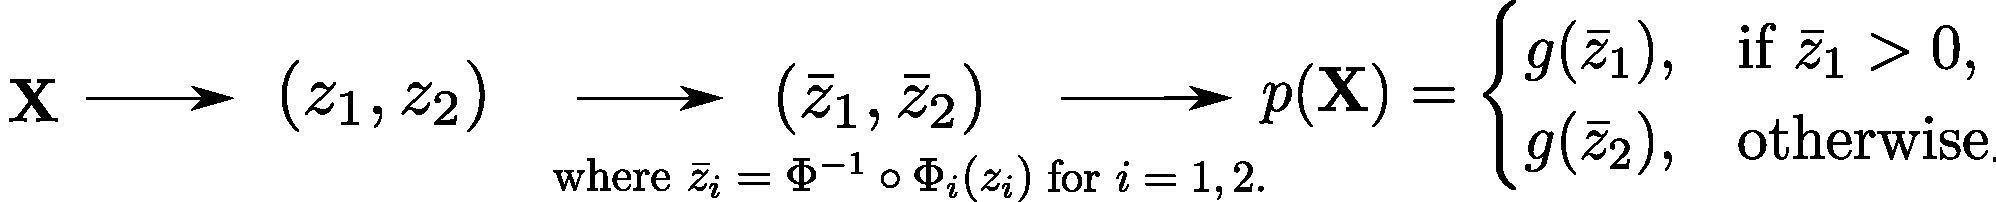
\includegraphics[width=.7\textwidth]{math.pdf}}

We set $\Phi_i = $ empirical CDF of $z_i$ for $i=1,2$; $\Phi = $ CDF of standard normal; $g(z)=(1+\exp(z))^{-1}$; matrix dimension $d=20,30,\ldots,60$; and training sample size $n=100, 150, \ldots, 400$. The construction of $\mu$ amounts to a high nonlinearity from $\mX$ to $\mu(\mX)$. Unlike parametric methods, the functional form of $\mu$ is set unknown to the algorithm. 

The first experiment assesses the impact of sample size to classification. We fix the matrix dimension $d=30$ and let the sample size $n$ increase. Figure~\ref{fig:logistic}a plots the resulting density of $\mu(\mX)$ induced from the nonlinear function $\mu(\cdot)$ and distribution of $\mX$. The classification error is measured by the excess risk $R(\hat S_{\text{bayes}})-R(\bayesS)$ evaluated on test data. As seen from Figure~\ref{fig:logistic}b, the classification error decays polynomially in sample size, which is consistent with our theoretical results. We find that a higher rank or a higher number of active nodes leads to a higher classification error, as reflected by the upward shift of the curve as $(r,s)$ increases. Indeed, a higher $(r,s)$ implies a higher complexity in the model space, thus increasing the generalization error of classification. 


The second experiment evaluates the impact of matrix dimension to classification accuracy. We fix the sample size $n=200$ and let the matrix dimension $d$ increase. Figure~\ref{fig:logistic}c plots the classification error versus the dimension $d$ for each of three model settings $(r,s)=(2,2), (2,3)$ and $(4,4)$. We find that the error increases slowly with matrix dimension, and the growth appears well controlled by the log rate. Note that, as the dimension increases, the number of active nodes remain unchanged, but the combinatoric complexity increases in the model space. The error seems unavoidable because of the price one needs to pay for not knowing the positions of the $s$ active nodes. The ability to effectively control massive noisy features highlights the benefit of our method in high dimensions. 

\begin{figure}[ht]
    \centering
    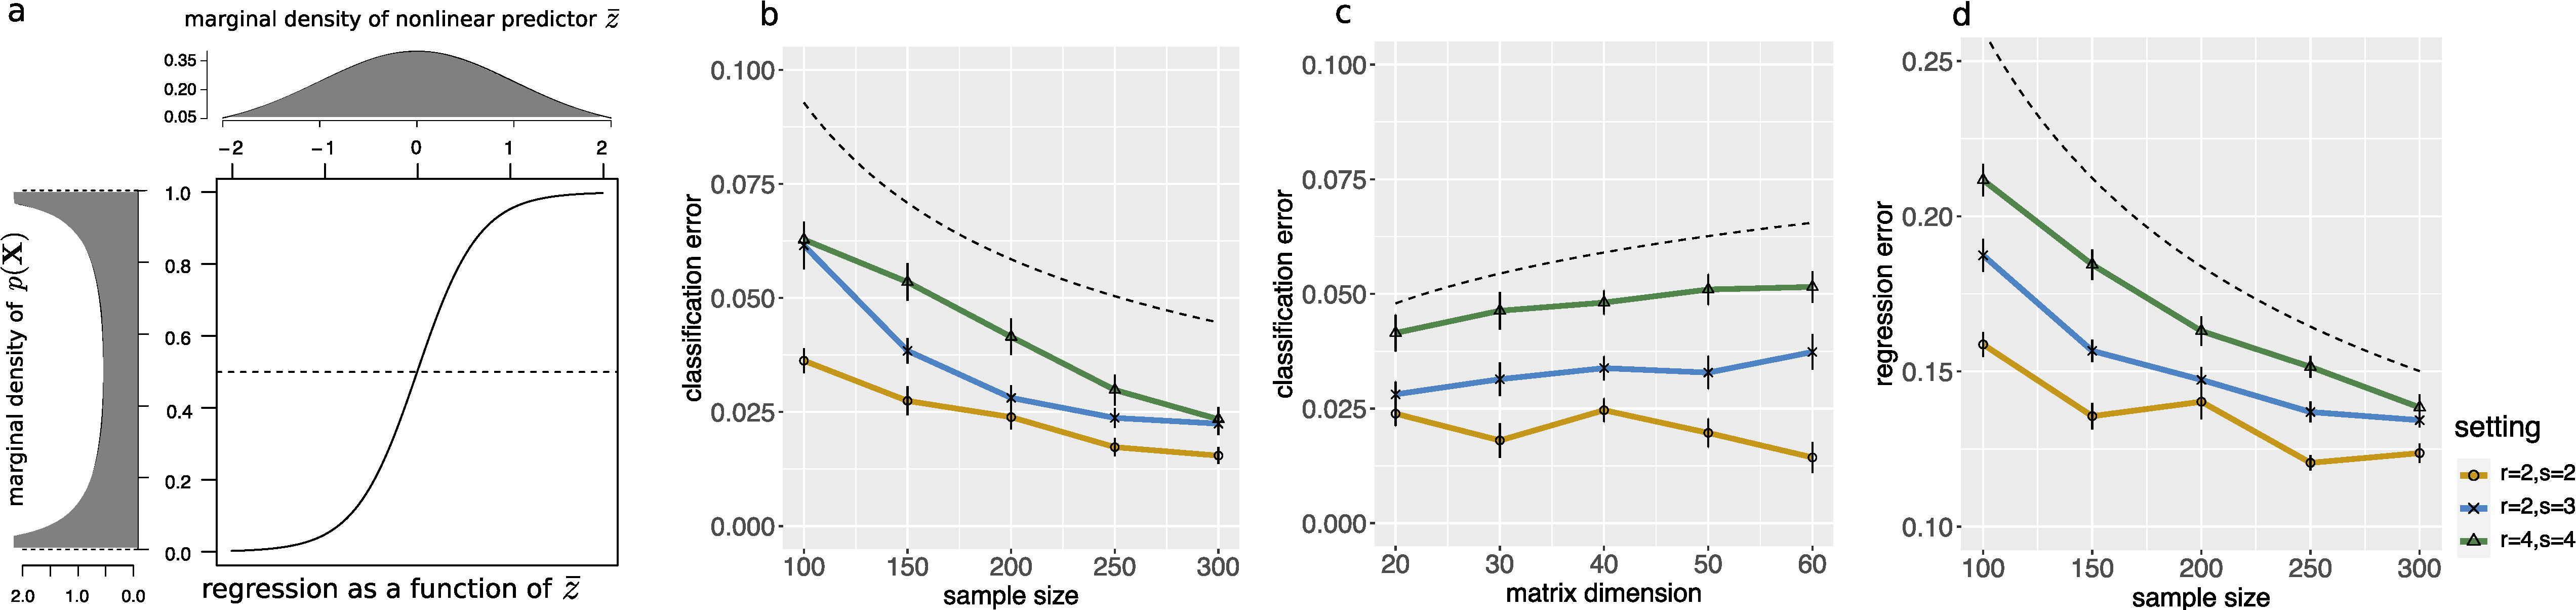
\includegraphics[width=\textwidth]{combined_logistic.pdf}
    \caption{Finite sample accuracy of matrix classification and regression. (a) simulation setup. (b) classification error with sample size when $d=30$. (c) classification error with matrix dimension when $n=200$. (d) regression error with sample size. The dashed line in panels (b)-(d) represent theoretical rates $\tO(n^{-2/3})$, $\tO(\log d)$, and $\tO(n^{-1/2})$, respectively. The reported statistics are averaged across 30 simulation replicates, with standard error given in the error bar.}\label{fig:logistic}
\end{figure}

The third experiment investigates similar aspects as before but to the task of matrix regression. We set the resolution parameter $H=20$ and aggregated the multiple level-sets as in our proposal~\eqref{eq:stepfunctionsample}. Figure~\ref{fig:logistic}d shows the regression error measured by $L$-1 risk, $\mathbb{E}|\hat \mu (\mX)- \mu(\mX)|$, evaluated on test data. Again, we see that the regression error decays polynomially in sample size. Note that our matrix-valued feature has ambient dimension $30\times 30=900$ whereas the sample size is on the order of hundreds. This scenario of high feature dimension low sample size is prevalent in brain network analysis. Nevertheless, our nonparametric method consistently learns the function $\mu$ from limited data without the need to specify a priori functional form.

\begin{figure}[ht]
    \centering
    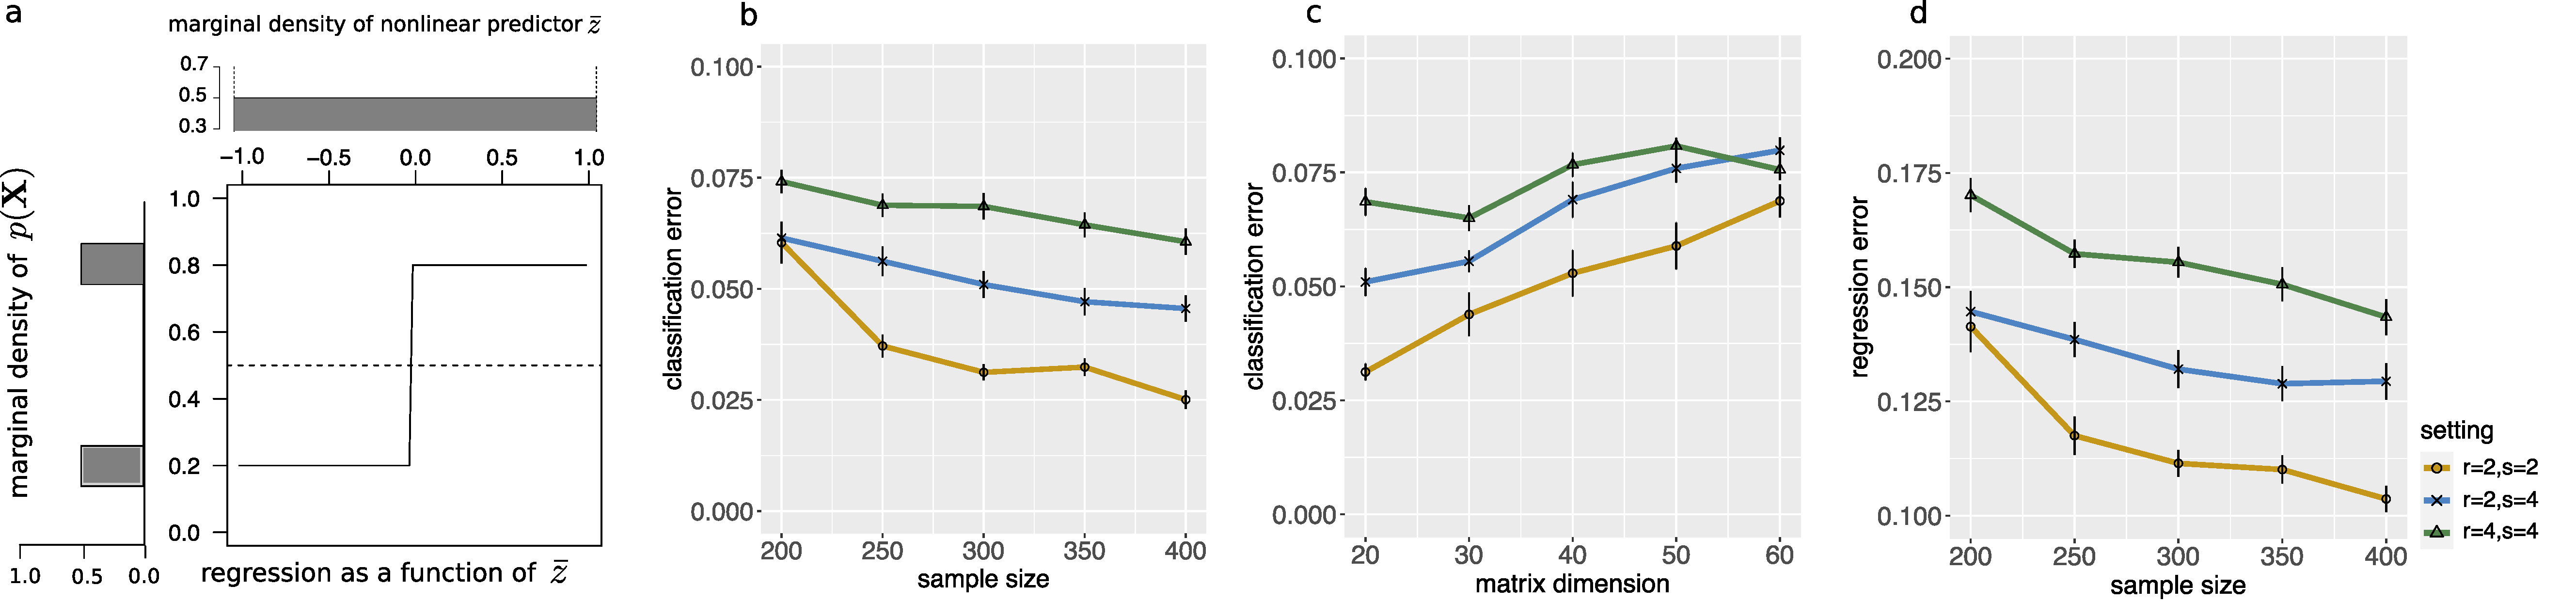
\includegraphics[width=\textwidth]{combined_steps.pdf}
    \caption{Finite sample accuracy under a different setting. (a) simulation setup. (b) classification error with sample size when $d=30$. (c) classification error with matrix dimension when $n=200$. (d) regression error with sample size. }\label{fig:step}
\end{figure}

The fourth experiment investigates the impact of target function to the prediction accuracy. We have shown that the probabilistic behavior of the random variable $\mu(\mX)$ plays a key role in our learning reduction (see Section~\ref{sec:idea}). Here we assess the empirical performance by repeating all the above experiments using a variety of $\mu(\mX)$. For space consideration, only one representative example is presented in the main texts, and the rest in the appendix~\ref{sec:sfigure}. Figure~\ref{fig:step}a shows a model setting that falls on the other end of the spectrum. The random variable $\mu(\mX)$ concentrates at two mass points $\pi=0.2$ and $0.8$. This makes the $\pi$-level set estimation challenging around $\pi=0.2$ and $0.8$, because of the nonidentifiability in the weighted classification. Interestingly, we find that our method maintains good performance on classification at $\pi=0.5$ (Figures~\ref{fig:step}b-c) and the overall regression (Figure~\ref{fig:step}d). One possible reason of this robustness is that we aggregate in total $(H-1)$ classifiers from $\Pi=\{{1\over H}, {2\over H},\ldots,{H-1\over H}\}$, each of which incurs at most ${1\over H}$ error to the function estimation. Therefore, the estimation is robust against off-target level sets, as long as the majority are accurate.  

\subsection{Comparison with other methods}\label{sec:comparison}
Next, we compare our method with several popular alternative methods:
\begin{itemize}[wide, labelwidth=!, labelindent=0pt]
\item Unstructured regular lasso ({\bf \small Lasso}). We vectorize the network predictor into a high-dimensional feature and then use elastic net~\citep{friedman2010regularization} with logistic loss to fit the vector-valued predictors.  
\item Parametric regression for network predictors with group lasso ({\bf \small LogisticM},~\cite{relion2019network}). The original proposal is designated for network classification, and we adopt the fitted value from logistic loss as the probability estimation. 
\item Convolutional Neural Network ({\bf \small CNN}) with two hidden layers implemented in Keras \citep{chollet2018deep}. We apply 64 filters with $3\times 3$ convolutional kernels to the matrix-valued predictor, followed by a pooling layer with size $5\times 5$. The resulting features (neurons) are fed to a fully connected layer of neural network with ReLU activation. 
\item {\bf \small Non}parametric {\bf \small MA}trix {\bf \small R}egression ({\bf \small NonMAR}). This is our method that uses level set approaches to estimate the regression function for matrix-valued predictors. 
\end{itemize}
We choose a range of representative methods and investigate the benefit of each approach. The \Lasso serves as a baseline to assess the gain of matrix-valued predictors over vector-valued predictors. The methods \CNN and \NonparaM are nonparametric approaches and \LogisticM is a parametric solution for matrix based prediction.  
\begin{figure}[ht]
    \centering
    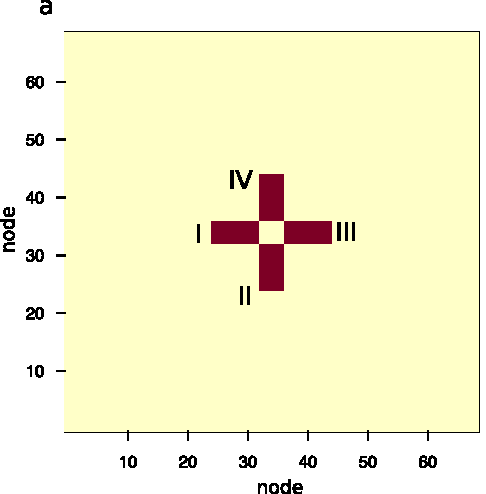
\includegraphics[width=3.8cm]{cross.pdf}
      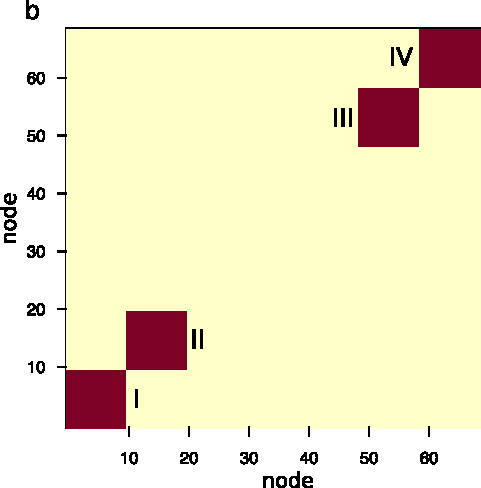
\includegraphics[width=3.8cm]{block.pdf}
        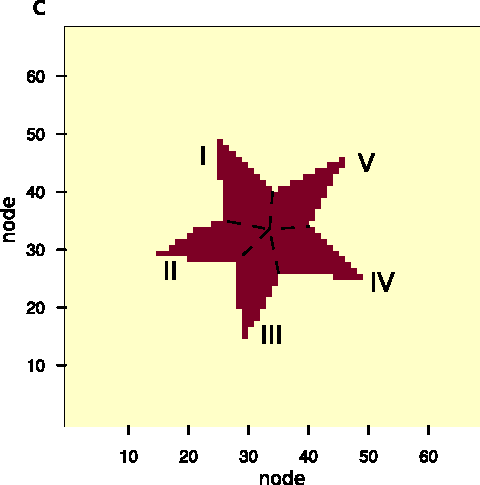
\includegraphics[width=3.8cm]{star.pdf}
          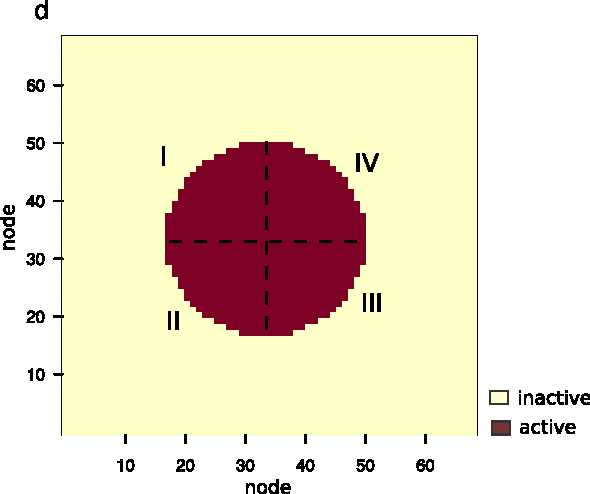
\includegraphics[width=4.7cm]{circle.pdf}
            
          \caption{Four active pattern in simulations. The active region is divided into four or five subregions (denoted I, II, ...), each of which has its own edge connectivity signal $g_{pq}(\pi)$.}\label{fig:region}
\end{figure}

For fair comparison, we adopt similar simulation setup as in~\cite{relion2019network}, except that we add more challenging network patterns in order to assess model misspecification. We simulate the data $(\mX_i, y_i)_{i=1}^n$ from latent variable model $(\mX,y)|\pi$ based on the following scheme (see details in Appendix~\ref{sec:joint}),
\[
\pi \stackrel{\text{i.i.d.}}{\sim} \text{Uniform}[0,1] \stackrel{\text{conditional on $\pi$}}{\longrightarrow}
\begin{cases}
y\sim \text{Ber}(\pi),\ \text{}y\perp \mX|\pi, \\
\mX=\entry{\mX_{pq}}, \ \text{where\ } \mX_{pq}\stackrel{\text{indep.}}{\sim} \tN(g_{pq}(\pi)\mathds{1}(\text{edge $(p,q)$ is active}), \sigma^2).
\end{cases}
\]
The edge connectivity signal, $g_{pq}(\pi)$, varies depending on the response probability $\pi$ and location of $(p,q)\in[d]^2$. Figure~\ref{fig:region} illustrates the active pattern which specifies the locations of active edges. The active region is further divided into several subregions, each of which has its own signal function $g_{pq}(\cdot)\colon [0,1]\to \mathbb{R}$. The function form of $g_{pq}(\cdot)$ is randomly drawn from a pre-specified library consisting of common functions such as $g(z)=\log(5z+1), 3\tan(z),6z^2,\ldots$. We set $d=68$, a training size $n=160$, and a test size $80$. 

Our simulation reflects the challenging heterogeneity commonly arisen in brain network analysis. The sample consists of a mixture of individual groups with varying response probability, and the network patterns vary from one group to another. Active brain regions are supported on a submatrix with typically unknown rank. In the noiseless case, the cross and block patterns are low-rank ($r = 3$ and 5, respectively), whereas the star and circle patterns are nearly full-rank (numerical rank $r\approx 30$ on the supported submatrix). In our simulation with noisy observation, we select the rank and sparsity parameters $(r,s)$ by 5-fold cross validation. The hyperparameters for the other three methods are selected by either default setting ({\bf \small LogisticM}) or cross validation ({\bf \small Lasso}, {\small \bf CNN}). We provide each algorithm the labeled networks as inputs after randomly permuting the node indices in the network. Because the software for \LogisticM supports symmetric matrices only, we provide the algorithm ${1\over 2}(\mX+\mX^T)$. 

\begin{figure}[ht]
    \centering
    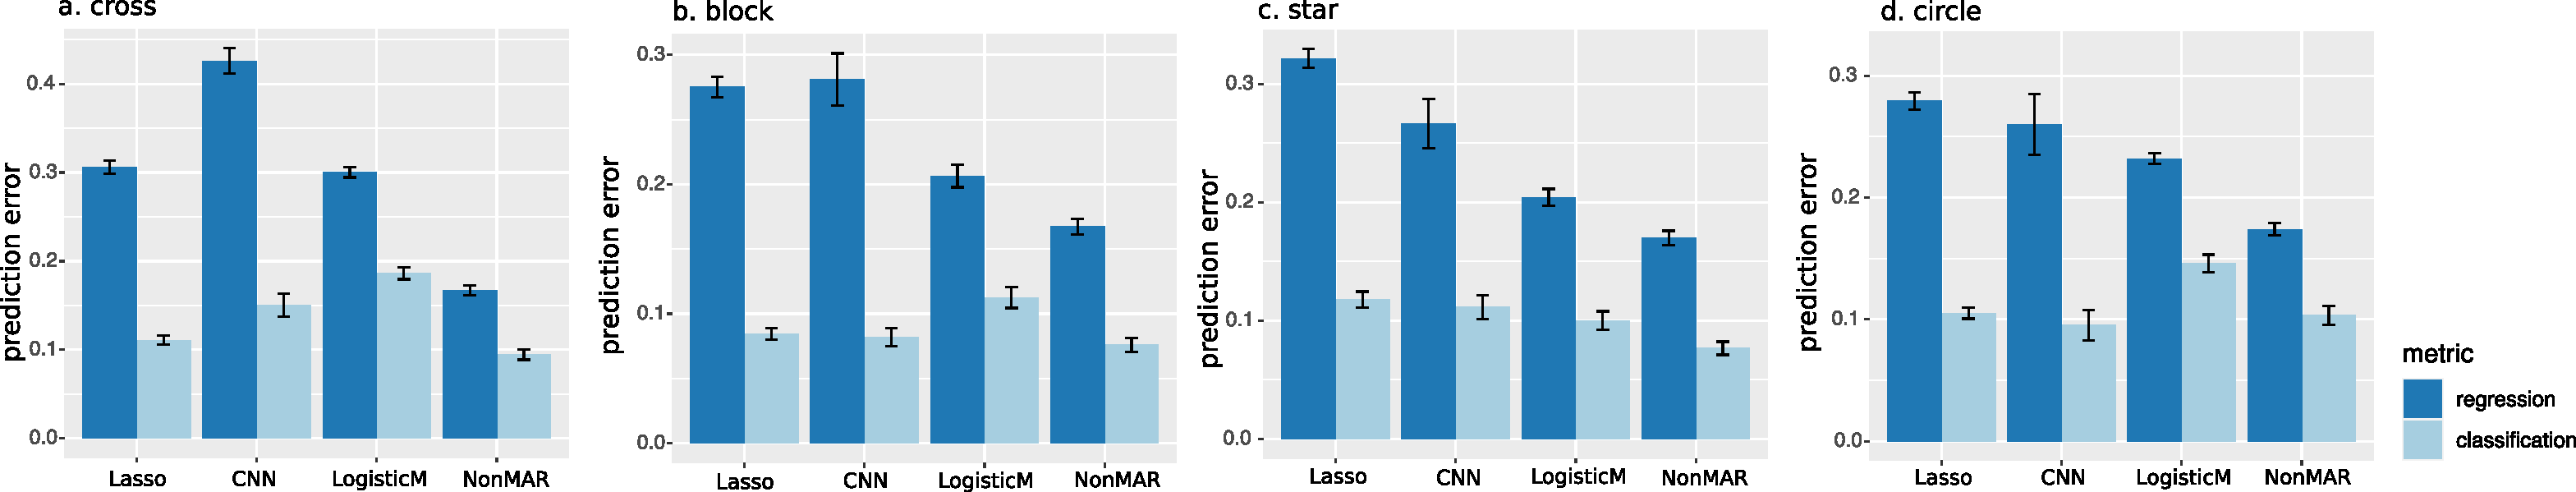
\includegraphics[width=\textwidth]{error_tot_comb2.pdf}
    \caption{Performance comparison between various methods under four different active patterns. }\label{fig:compare}
\end{figure}

Figure~\ref{fig:compare} compares the out-of-sample prediction between different methods. We focus on the regression problem and assess the performance using test data. We find that \NonparaM consistently outperforms others, and the reduction in error is substantial. For example, the relative reduction using \NonparaM over the next best approach, {\bf \small LogisticM}, is over 20\% for patterns a and d, and over 15\% for patterns b and c. The results show the benefit of our nonparametric approaches by allowing more flexible functional space. Furthermore, we find that neither \Lasso nor \CNN has satisfactory regression performance. One possible reason is that these two methods fail to appropriately incorporate the network structure of the predictors. The \Lasso takes vectorized matrices as inputs and therefore losses the two-way pairing information. On the other hand, \CNN assumes spacial ordering within row/column indices. Although local similarity is an appropriate model for common imaging analysis, the row/column indices are meaningless for networks. Indeed, adjacency matrices differ by row/column permutation represent the same network, and methods that are index-invariant (\LogisticM and {\bf \small NonMAR}) show better performance. Our simulations cover a reasonably broad range of network models with rich structure. The results demonstrate the advantages of our nonparametric approach on the task of network regression. 

We also report the accuracy on classification which is an intermediate step of regression. Figure~\ref{fig:compare} shows the favorable performance of our method especially when compared to {\bf \small LogisticM}. Among the four models of active regions, our method performs the best in all three. The only exception is the circle pattern where the \CNN has a lower classification error by a slight margin. This is perhaps due to the fact that circle pattern is nearly full rank which favors complicated models such as {\bf \small CNN}. Nevertheless, our method \NonparaM achieves stable performance in spite of its simplicity. Interestingly, we find that the benefit of our method is more substantial in regression than in classification. One possible reason is that classification is an easier problem and less sensitive to various approaches. The result also suggests that the main reason of our method's superior regression performance may be attributable to level set aggregations. 

\begin{figure}[ht]
    \centering
   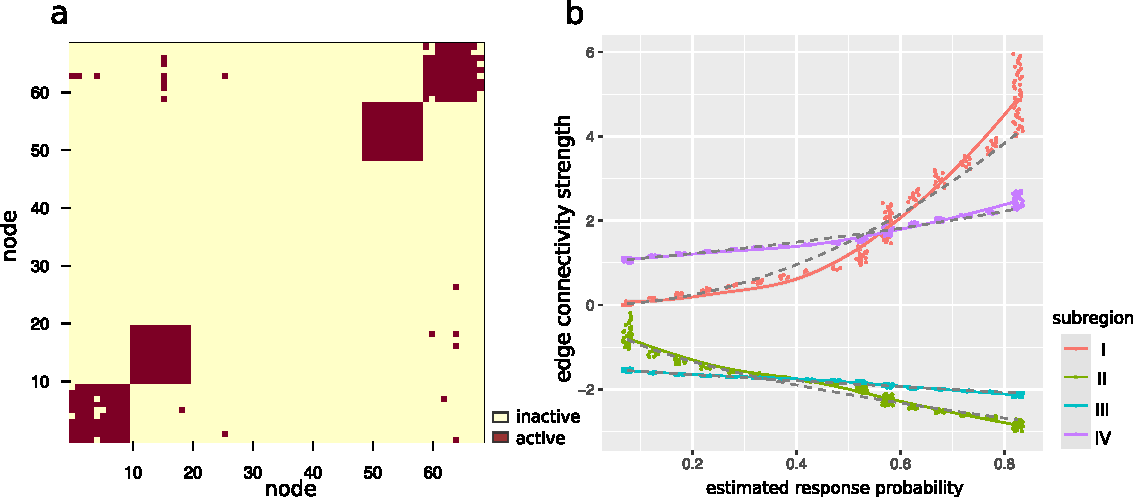
\includegraphics[width=8.1cm]{est_block.pdf}
          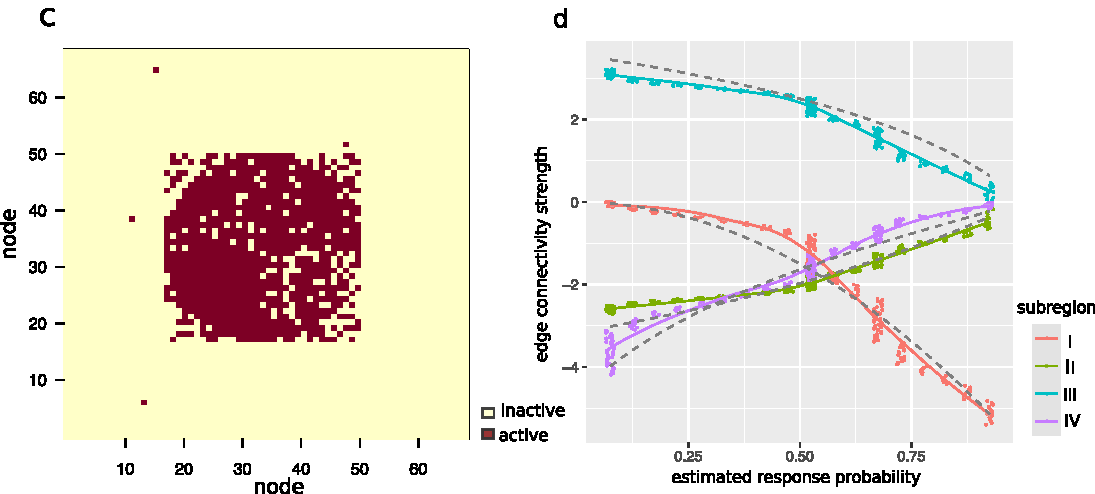
\includegraphics[width=8.1cm]{est_circle.pdf}
 \caption{Example outputs returned by {\bf \small NonMAR}. Panels (a) and (c) plot the top edges selected by our method. Panels (b) and (d) are scatter plots of the edge connectivity strength (averaged by subregion) versus the estimated response probability. The ground truth function is depicted in dashed curve.}\label{fig:compare2}
\end{figure}


We provide illustrate examples to show the outputs returned by {\bf \small NonMAR}. Figures~\ref{fig:compare2}a and c plot the top edges selected by \NonparaM based on the moving averages of feature weights $(\hat \mB_\pi)_{\pi\in\Pi}$ with $\Pi = \{0.2,\ldots,0.8\}$. The selected region agrees well with the ground truth (Figures~\ref{fig:compare}a and c). We also investigate the relationship between edge connectivity for individual $i$ and the estimated response probability $\hat \pi_i$ (Figures~\ref{fig:compare2}b and d). The trajectory of the edge connectivity accurately resembles the ground truth function in each subregion. The results demonstrate that our method is able to recover the right ``sorting'' of individuals with respect to the response probability on a continuous spectrum. 
The successful recovery of complicated unknown functions makes our method {\bf \small NonMAR} appealing in applications. 

\subsection{human brain connectome data}\label{sec:real}
We apply our method to brain network data from Human Connectome Project (HCP)~\citep{van2013wu}. The HCP is a recent consortial effort that aims to understand the relationships between brain connectivity and human traits. The dataset consists of brain connectivity networks from a sample of healthy individuals. The connectivity networks were preprocessed following a standard pipeline~\citep{zhang2018mapping}, and the brain was parcellated to 68 regions-of-interest following the Desikan atlas~\citep{desikan2006automated}. Each brain network is represented as a 68-by-68 binary matrix, where the entries encode the presence or absence of fiber connections between the 68 brain regions. In addition, a range of cognitive, motor, sensory, and emotional scores are measured for each individual. 

We analyze the Variable Short Penn Line Orientation Test (VSPLOT) score which measures the individual's visuospatial processing ability. In VSPLOT, two line segments are presented on the screen, and individuals are asked to rotate a movable line to make it parallel to the fixed line~\citep{moore2015development}. We use the dataset processed by~\cite{wang2019common}, and analyze $n=212$ individuals whose VSPLOT scores are either high ($y=1$) or low ($y=-1$). We adjust age and gender as additional covariates in the prediction, and use a random 60-20-20 split of the data for training, validation, and testing. 

%\normalsize
%\begin{table}
%\resizebox{.45\textwidth}{!}{
%\begin{tabular}{c|cc}
%\hline
%Method &  AUC  & \% of Active Nodes\\
%\hline
%{\bf \small NonMAR-p} &{\bf 0.73 (0.03)} &88.2   \\
%{\bf \small NonMAR}& {\bf 0.77 (0.04)}  &97.3 \\
% LogisticM&0.72 (0.02)& 100.0\\
%    Lasso&0.68 (0.01)&89.7\\
 % CNN&0.67 (0.03)&-$^{}$\\
%   \hline
%\end{tabular}
%}
%\vspace{.5cm}
%{\small \\
%Note: CNN dost not report summary statistics for node selection.\\
%Numbers in parentheses are standard errors over 5-fold cross validation. }\\
%\resizebox{.45\textwidth}{!}{
%\begin{tabular}{c|ccc}
%\hline
%Rank &Node &  Node& $p$-value$^*$ \\  
%\hline
%1&r-inferiortemp$^{**}$&r-middletemp&$0.01$\\
%2&r-pars&r-supra&3e-5\\
%3&r-posterior&l-precentral&0.01\\
%4& l-caudal& l-isthmus&2e-5\\
%\hline
%\end{tabular}\\
%}
%\vspace{.4cm}
%{\small \\
%$^*$ calculated from two sample test based on two label groups. %\\
% $^{**}$ Node names are shown in abbreviations, with ``r'' and ``l'' indicating the right and left hemisphere, respectively.  }
%\end{table}

\begin{figure}[ht]
    \centering
       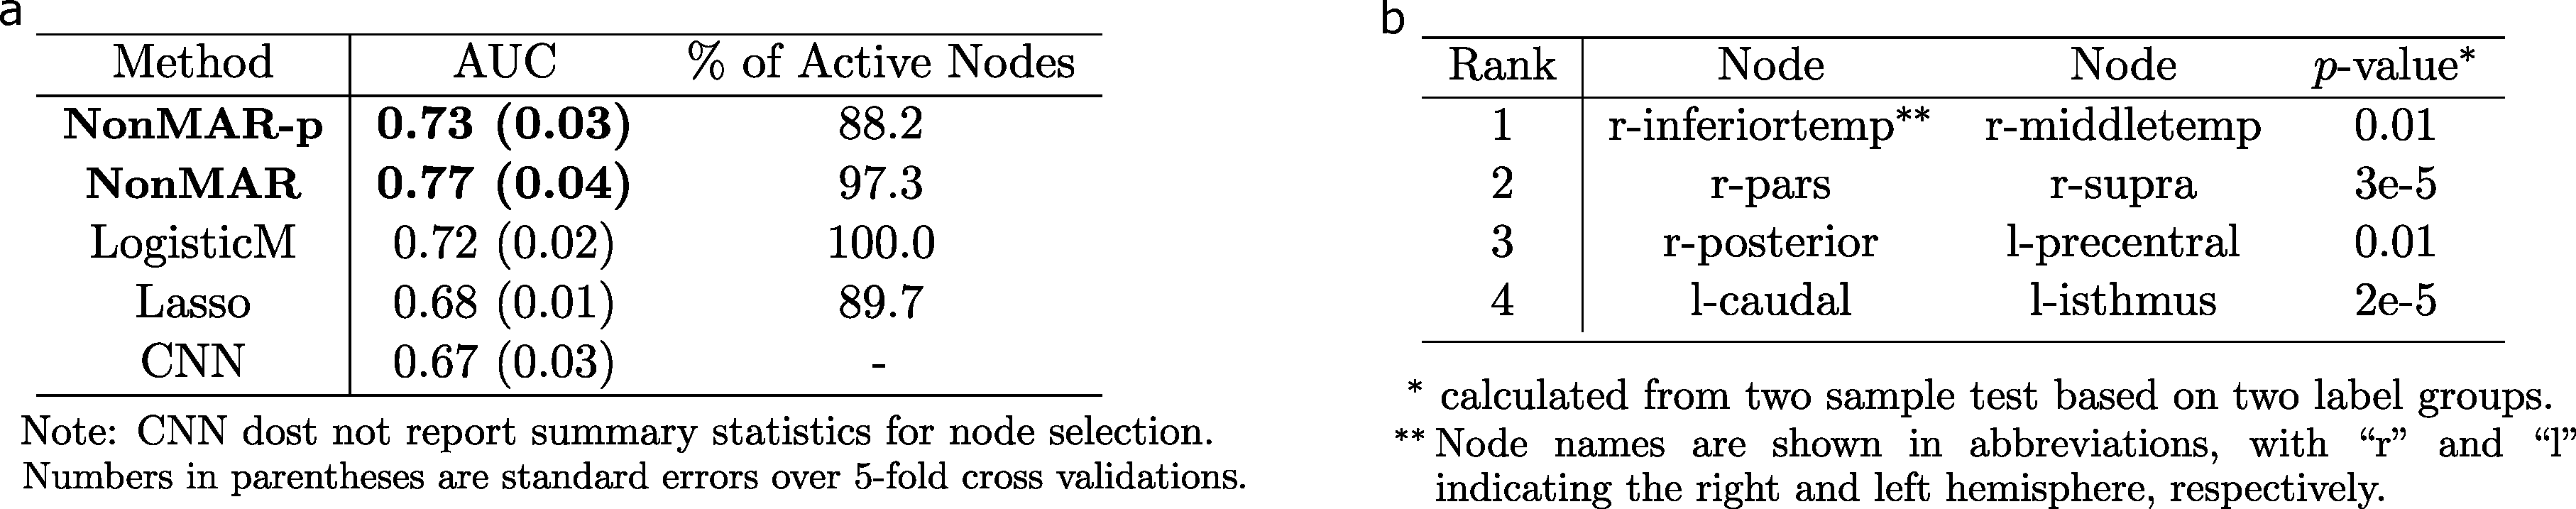
\includegraphics[width=\textwidth]{braintable.pdf}
 \caption{HCP analysis results based on our method {\bf \small NonMAR}. (a) Comparison of prediction accuracy. (b) Top edges selected by our method {\small \bf NonMAR-p}. }\label{fig:real}
\end{figure}

We compare our performance to other methods using the same procedure as in the previous section. Figure~\ref{fig:real}a shows that our method achieves high regression accuracy, measured by area under receiver operating characteristic (AUC). As common in high-dimensional settings, we observe that models with optimal cross-validation accuracy tend to include many noise variables. A useful heuristic is the so-called ``one-standard-error rule''~\citep{hastie2015statistical}, in which one selects the most parsimonious model with cross-validation accuracy within one standard error of the best. We apply this rule and report the results as {\bf \small NonMAR-p}. It is remarkable to see that {\bf \small NonMAR-p} results in 12\% reduction of active nodes but still achieves excellent accuracy (AUC = 0.73). 

\begin{figure}[ht]
    \centering
       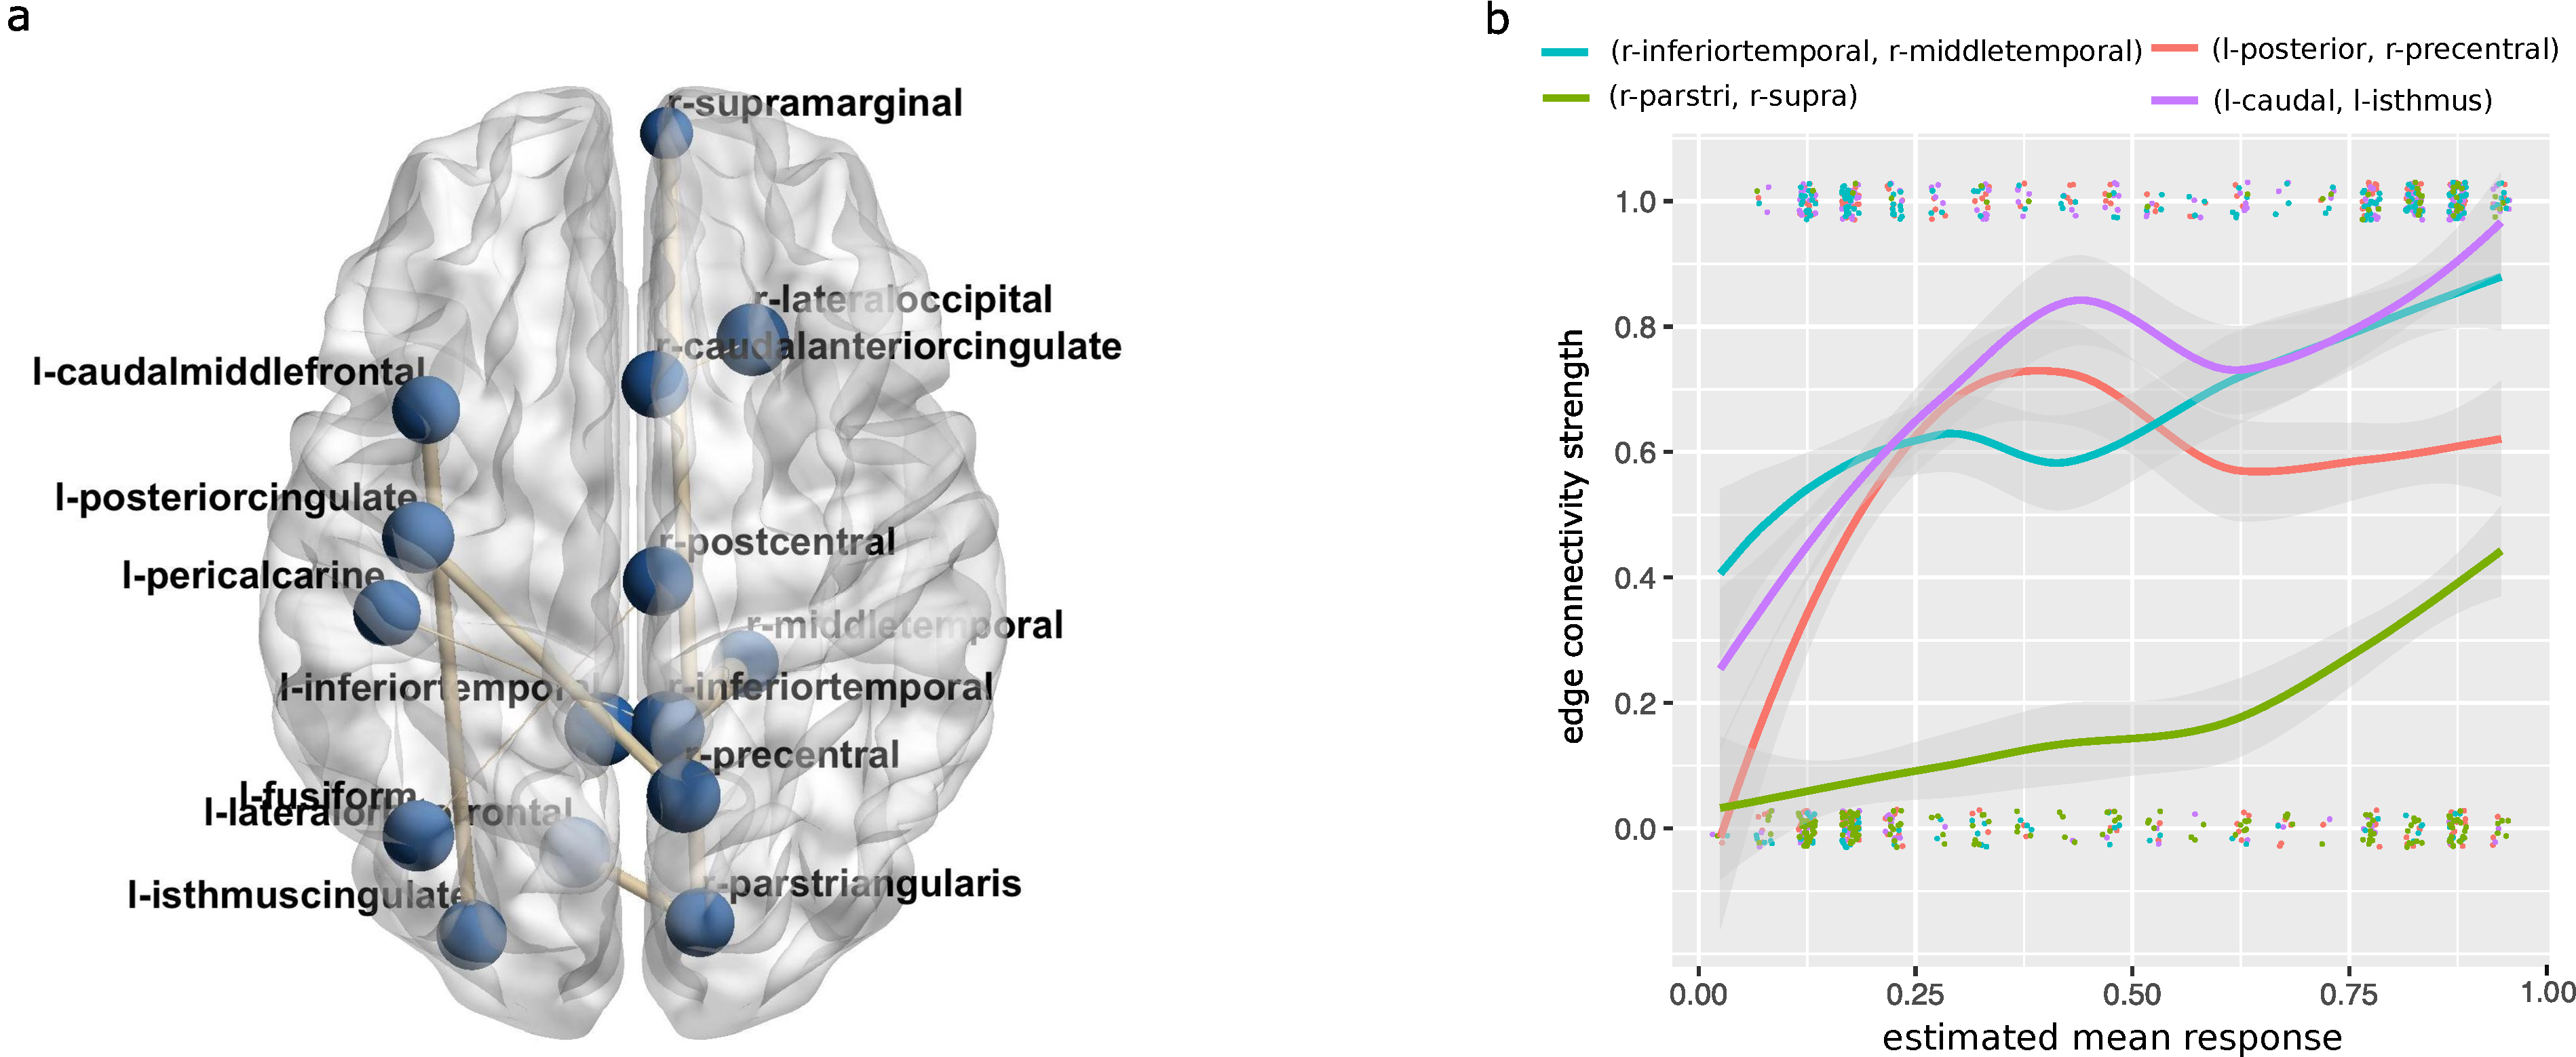
\includegraphics[width=1\textwidth]{brain.pdf}
 \caption{HCP analysis results based on our method {\bf \small NonMAR}.  (a) Top edges overlaid on brain template. (b) Edge connectivity strength versus estimated response probability. Colored curves represent the moving averages of connectivity strengths, gray bands represent one standard error, and jitter points represent the raw connectivity values (0 or 1). }\label{fig:real2}
\end{figure}


Figure~\ref{fig:real}b lists the top brain edges identified by our method. Edges are ranked by their maximal values in the feature weights $(\hat \mB_\pi)_{\pi \in [0,1]}$ via moving averaging. We find that the top edges involve connections between frontal and occipital regions in the right hemisphere (Figure~\ref{fig:real2}a). This seems consistent with recent evidence of dysfunction in right posterior regions for deficits in visuospatial processing~\citep{wang2019common}. We also find nonlinear relationship between edge connection strength and response probability. In Figure~\ref{fig:real2}b, the connection (r-parstriangularis, r-supramarginal) grows slowly when $\pi$ is low but fast when $\pi$ is high. In contrary, the connection (r-posteriorcingulate, r-precentral) grows fast initially and then reaches a plateau as $\pi$ increaases. The detected pattern reveals the heterogeneous changes in brain connectivities with respect to visuospatial processing ability. 


\section{Discussion}
We have developed the learning framework for the relationship between a binary label response and a high-dimensional matrix-valued predictor. 
Our method respects the matrix structure of the predictors and provide interpretable prediction via a nonparametric approach. 
The theoretical and numerical results demonstrate the competitive performance of our method.

Our work unlocks several directions of future research. 
Although we have presented the work in the context of matrix-valued predictors, we may consider extensions to other nonconventional predictors, such as images, graphs, tensors, functional time-series, and so on. Recent research has shown fruitful results in classification tasks with nonconventional predictors~\citep{wang2016classification,arroyo2020simultaneous}. Our proposed reduction approach provides a potential building block for more challenging regression tasks. It is also worthy noting that each of the aforementioned predictors may processes its own special structure depending on the applications. Exploiting the benefits and properties of nonparametric regression in the specialized tasks warrants future research. 

We may also ask whether the results here, provided in the setting of binary regression with $y\in\{-1,1\}$, may be extended to a continuous response $y\in\mathbb{R}$. The answer is affirmative if we assume the response $y$ is bounded, e.g.\ $y\in[-L,L]$, for $L>0$. One possible solution is to use response-dependent weight in place of response-dependent weight in the classification. Specifically, for a fixed target level $\pi\in [-L,L]$, define a new binary response $\tilde y = \sign (y-\pi)$, a response-dependent weight $\tilde  w_\pi(y)=|y-\pi|$, and a general weighted classification risk
\begin{equation}\label{eq:continuousrisk}
\tilde R_\pi(S)\stackrel{\text{def}}{=}\mathbb{E}\left[\tilde  w_\pi(y)\mathds{1}(\tilde y \neq \sign (\mX\in S))\right].
\end{equation}
The risk~\eqref{eq:continuousrisk} extends the $\pi$-weighted classification risk~\eqref{eq:risklevel} for a continuous response, where the weight $\tilde  w_\pi(y)=|y-\pi|$ is the distance from the response $y$ to the target level $\pi$. Importantly, the level set $S(\pi)=\{\mX\in \tX \colon \mu(\mX)\geq \pi\}$ is the global minimum of~\eqref{eq:continuousrisk} under conditional model of the type $y|\mX=\mu(\mX)+\varepsilon$, where the noise $\varepsilon$ is a mean-zero random variable whose distribution is allowed to depend on $\mX$~\citep{willett2007minimax,scott2007regression}. With this statistical characterization, our main result on excess regression risk bound in Section~\ref{sec:idea} still holds. Therefore, our learning reduction approach equally applies to a continuous response by using $\tilde w_\pi(y)$ and $\tilde y$ in place of $w_\pi(y)$ and $y$, respectively. For an unbounded response, it is unclear whether the level set approach still achieves accuracy guarantees. We leave these questions for future work. 

%Our regression approach also provides flexibility to local function estimation. In geographical applications, for example, people are interested in detecting the minima and maxima of a nonparametric function. In these applications, the entire region is less interested, but a restricted range, $[L_1, L_2]$, may be more relevant. Then our method is be used to learn this function in a given range only. Furthermore, the adaptive resolution parameter adaptive to the changing behavior of functional is of future interest. Application to adaptive level set estimation and functional minima and maxima detection warrants future research.

%Lastly, from computational perspective, the two-way sparse and low rank ..., and we find in practice it provides better accuracy in real applications. Convex surrogate is also possible, for example, by nuclear norm and group lasso. Recent development has shown the empirical superior of nonconvex approach, while at the cost of harder theoretical analysis. The balance between practical feasibility and analytical guarantees warrants future research.
\bibliographystyle{chicago}

\bibliography{tensor_wang}



\clearpage
\section*{Appendix}
\addcontentsline{toc}{section}{Appendices}
\renewcommand{\thesubsection}{\Alph{subsection}}
\setcounter{figure}{0}
\setcounter{table}{0}
\renewcommand{\thetable}{S\arabic{table}}
\renewcommand{\thefigure}{S\arabic{figure}}
\renewcommand{\figurename}{Supplemental Figure}
\renewcommand{\tablename}{Supplemental Table}


\subsection{Connection to joint matrix decomposition with functional coefficients}\label{sec:joint}
In the main text, we have shown that our classifier functions $\tF(r,s_1,s_2)$ incorporates certain retrospective models $\mX|y$. Here we extend the retrospective model to a more general family  which we coin as ``functionally decomposable matrices''. The model essentially extends Example~\ref{example2} from two classes of $\mX$ to a series of $\mX$ on a continuous spectrum of $\pi$. 

\begin{example}[Functionally decomposable matrices]\label{ex:matrix_decomposition}
We consider a matrix model $\mX_\pi\stackrel{\text{def}}{=}\mB_0+ \sum_{s\in[r]}g_s(\pi)\mB_s+\sigma \mE$, where $\pi \in[0,1]$ is a real-valued index; $\mE$ is a noise matrix consisting of i.i.d.\ entries in $N(0,1)$; $\sigma$ is the noise level; $\mB_0$ is an arbitrary baseline matrix; $(\mB_s)_{s\in[r]}$ is a set of rank-1 matrices in $\{0,1\}^{d_1\times d_2}$ that satisfy (i) non-overlapping supports, i.e., $\langle \mB_s, \mB_{s'}\rangle=0$ for all $s\neq s'$, and (ii) bounded total support, i.e., $\sum_{s\in[r]}\text{supp}(\mB_s)\leq (s_1,s_2)$; and the coefficients $g_s(\cdot)\colon [0,1]\to\mathbb{R}$ are monotonic functions with respect to $\pi$ for all $s\in[r]$. 

Now, suppose the observation takes the form of pair $(\mX_\pi,y_\pi)$ with $y_\pi \sim \text{Ber}(\pi)$, where $y_\pi$ is conditionally independent of $\mX_\pi$ given $\pi$, and $\pi\in[0,1]$ is drawn from an unknown distribution over $[0,1]$. Equivalently, the generative model is expressed in the following scheme:
\[
\pi \stackrel{\text{i.i.d.}}{\sim} \text{Uniform}[0,1] \stackrel{\text{conditional on $\pi$}}{\longrightarrow}
\begin{cases}
y\sim \text{Ber}(\pi),\ y\perp \mX|\pi, \\
\mX=\mB_0+\entry{\mX_{pq}},
\end{cases}
\]
where $ \mX_{pq}\stackrel{\text{indep.}}{\sim}\tN(g_{s}(\pi), \sigma^2)$ if  the position $(p,q)$ falls in the support of $\mB_s$ and $ \mX_{pq}\stackrel{\text{indep.}}{\sim}\tN(0,\sigma^2)$  otherwise.  Recall that $\mu(\mX)=\mathbb{E}(y|\mX)$. In the noiseless case $\sigma = 0$, there exists a sequence of functions $(f_\pi)_{\pi\in(0,1)}$ with $f_\pi \in\tF(r,s_1,s_2)$, such that $\sign (\mu(\mX)-\pi) = \sign f_\pi(\mX)$ for all $\pi \in (0,1)$.

The above example shows the connection of our method to joint decomposition of matrices $(\mX_\pi)_{\pi\in[0,1]}$. We should point out, despite of the seeming similarity, a fundamental challenge arises in our setting when the latent index $\pi$ is unobserved. Our level-set approach essentially learns the right ``sorting'' of $\mX_\pi$ against the index $\pi\in[0,1]$ (see Figure~\ref{fig:method}), thereby facilitating the joint estimation of matrix basis $\mB_s$ and relationship $\pi=\pi(\mX)$. 
\end{example}


Furthermore, we provide additional results on the low-rank two-way sparse classifiers. The following proposition gives a sufficient condition for exact recovery of level sets through halfspaces.
%; the results show that what essentially matters is the boundary of level sets.  where $S(\pi)$ be the level set defined in~\eqref{eq:level} and $\bar S(\pi)$ be the classifier defined in~\eqref{eq:optimization} optimized over $\tF(r,s_1,s_2)$. 

\begin{prop}[Low-rank and sparse boundaries]\label{prop:px} Let $\mu(\mX)$ be a regression function continuous in $\mX\in\mathbb{R}^{d_1\times d_2}$. Suppose that there exists a low-rank two-way sparse matrix $\mB_\pi$ and a real value $b_\pi\in\mathbb{R}$, such that the boundary set $\partial S(\pi)=\{\mX\colon \mu(\mX)=\pi\}$ is included in the set $\{\mX\colon \langle \mX, \mB_\pi \rangle = b_\pi\}$. Then $\sign (\mu(\mX)-\pi)=\sign (f_\pi(\mX))$ for some $f_\pi(\mX)\in \tF(r,s_1,s_2)$. Note that $(\mB_\pi, b_\pi)$ is allowed to vary depending on $\pi$. 
\end{prop}

\begin{proof}[Proof of Proposition~\ref{prop:px}]
For given $\pi\in\Pi$, suppose $\partial S(\pi) = \{\mX\colon \mu(\mX) = \pi\} = \{\mX:\langle \mB_\pi,\mX\rangle = b_\pi\}.$
Define two open sets $S_1$ and $S_2$ as 
\begin{align}
S_1(\pi) = \bar S(\pi)\setminus \partial S(\pi) = \{\mX\colon \langle \mB_\pi,\mX\rangle >b_\pi\}\quad\text{ and }\quad S_2(\pi) = \bar S^c(\pi) = \{\mX\colon \langle \mB_\pi,\mX\rangle < b_\pi\}.
\end{align}

First, we prove that there is no $\mX_1,\mX_2\in S_i(\pi)$ such that $p(\mX_1)>\pi$ while $p(\mX_2)<\pi$ for $i = 1, 2.$ To be specific, $S_i(\pi)$ is included either $S(\pi)\setminus\partial S(\pi) = \{\mX\colon \mu(\mX)>\pi\}$ or $S^c(\pi) = \{\mX\colon \mu(\mX)<\pi\}.$ 

It suffices to show the case $S_1(\pi)$.
Without loss of generality, suppose that there is $\mX_1,\mX_2\in S_1(\pi) $ such that $p(\mX_1)>\pi$ and $p(\mX_2)<\pi$. 
We can always find $\mX_3 = \lambda \mX_1+(1-\lambda)\mX_2$ for some $\lambda\in(0,1)$ such that $p(\mX_3) = \pi$ by continuity of $\mu(\mX).$ Because $p(\mX_3) = \pi$, we have  $\mX_3\in \partial S(\pi) = \{\mX\colon \mu(\mX) = \pi\} =  \{\mX\colon\langle \mB_\pi,\mX\rangle = b_\pi\}$. However, this contradict the fact \[\langle \mB_\pi,\mX_3\rangle =\lambda \langle \mB_\pi,\mX_1\rangle + (1-\lambda)\langle \mB_\pi,\mX_2\rangle> \lambda b_\pi+(1-\lambda)b_\pi = b_\pi. \]
Therefore, there is no $\mX_2\in\bar S_1(\pi)$ such that $p(\mX_1)<\pi$. 

Second, we prove that there are only two cases that 
\begin{enumerate}
    \item[(C1):]$S_1(\pi) = \{\mX\colon \mu(\mX) >\pi\} \text{ and } S_2(\pi) = \{\mX\colon \mu(\mX) <\pi\}$.
    \item[(C2):]$S_1(\pi) = \{\mX\colon \mu(\mX) <\pi\} \text{ and } S_2(\pi) = \{\mX\colon \mu(\mX) >\pi\}$.
\end{enumerate}
Suppose $S_1(\pi)\subset \{\mX\colon \mu(\mX)>\pi\}$. Since $\{\partial S(\pi),S_1(\pi),S_2(\pi)\}$ is a partition of $\mathbb{R}^{d_1\times d_2}$ and both $\{\mX\colon \mu(\mX)>\pi\}$ and $\{\mX\colon \mu(\mX)<\pi\}$ are non-empty set, only possible case is (C1). Similarly, if $S_2(\pi) \subset\{\mX\colon \mu(\mX)<\pi\}$, only possible case is (C2).

Notice that (C1) is equivalent to $S(\pi) = \bar S(\pi)$ while (C2) is equivalent to $S(\pi) = \bar S^c(\pi).$
\end{proof}



\clearpage
\subsection{Supplementary figures}\label{sec:sfigure}
     \begin{figure}[ht]
    \centering
    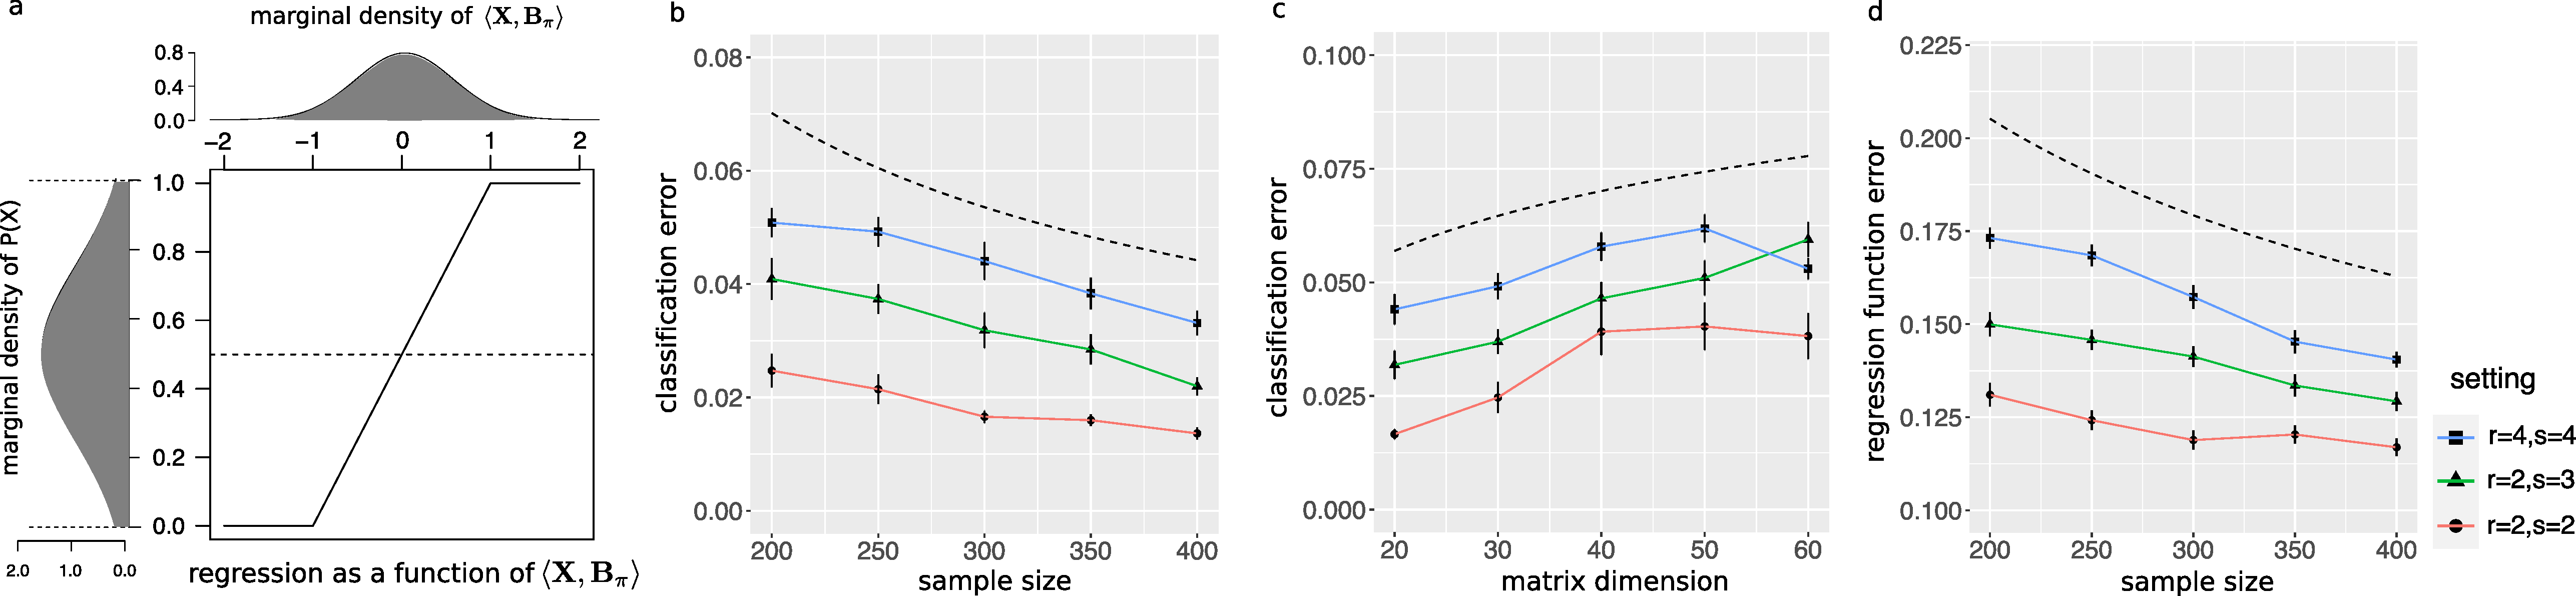
\includegraphics[width=16cm]{combined_linear.pdf}
    \caption{Finite sample accuracy of matrix classification and regression. (a) simulation setup. (b) classification error with sample size when $d=30$. (c) classification error with matrix dimension when $n=200$. (d) regression error with sample size. 
    The dash line in panels (b)-(d) represent theoretical rate $\tO(n^{-2/3})$, $\tO(\log d)$, and $\tO(n^{-1/3})$, respectively. }\label{fig:linear}
\end{figure}

\begin{figure}[ht]
    \centering
   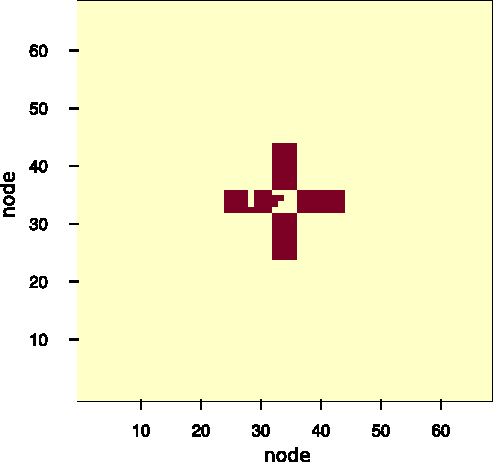
\includegraphics[width=3.7cm]{est_cross.pdf}
      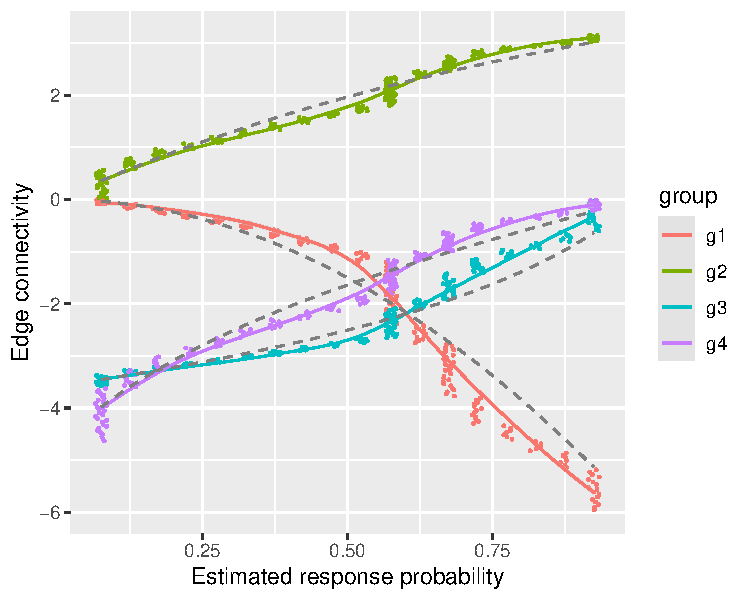
\includegraphics[width=4.3cm]{FMD_cross.pdf}
          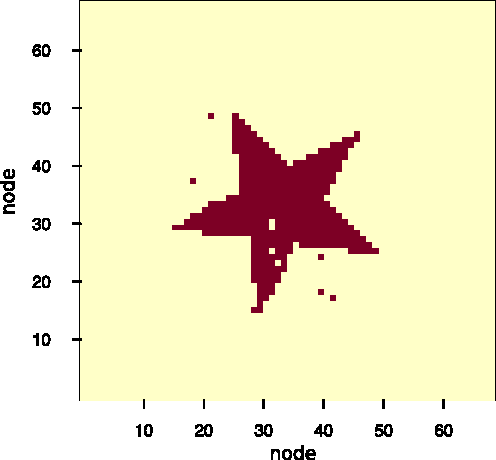
\includegraphics[width=3.7cm]{est_star.pdf}
               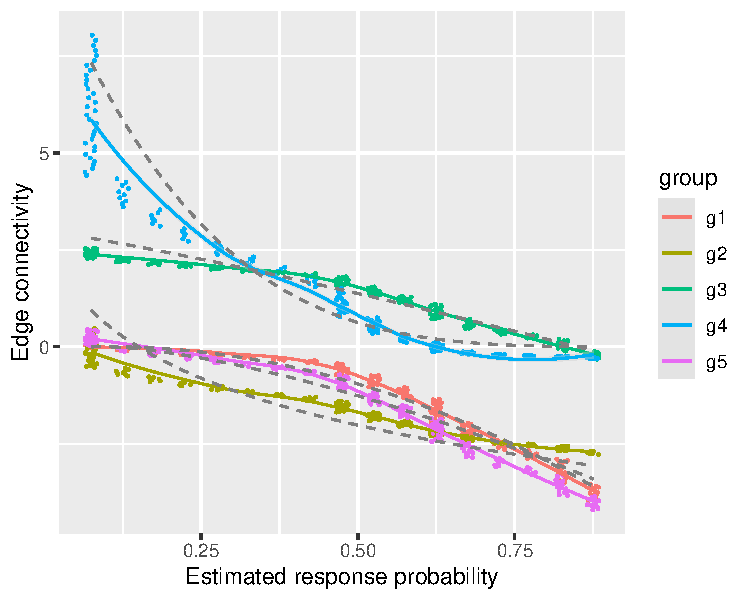
\includegraphics[width=4.3cm]{FMD_star.pdf}
 \caption{Example outputs returned by {\bf \small NonMAR}. Panels (a) and (c) plot the top edges selected by our method. Panels (b) and (d) are scatter plots of the edge connectivity strength (averaged by subregion) versus the estimated response probability. The ground truth function is depicted in dashed curve.}\label{fig:compare3}
\end{figure}


\clearpage
\subsection{Proofs}
\subsubsection{Proof of Proposition~\ref{thm:identifiability}}
\begin{proof}[Proof of Proposition~\ref{thm:identifiability}]
For ease of notation, we drop the argument $\pi$ from $S_{\text{bayes}}(\pi)$, $R_\pi(\cdot)$, and $d_\pi(\cdot,\cdot)$, and simply write $S_{\text{bayes}}$, $R(\cdot)$, and $d(\cdot,\cdot)$ respectively. The following identity is useful to relate the excess risk and set difference in classifiers,
\begin{align}\label{eq:excess}
d(S,\bayesS) &\stackrel{\text{def}}{=} R(S)-R(\bayesS)\\
& = \mathbb{E}_{\mX,y}\left[w(y)\mathds{1}(y\neq I(S))\right]-\mathbb{E}_{\mX,y}\left[w(y)\mathds{1}(y\neq I(\bayesS))\right]\notag \\
&=\mathbb{E}_{\mX}\left[(\pi-\mu(\mX))\left(I(S)-I(\bayesS)\right)\right]\notag \\
&=2\int_{\mX\in S\Delta S_{\text{bayes}}}|\mu(\mX)-\pi|d \mathbb{P}_{\mX}.
\end{align}

We divide the proof into two cases: $\alpha \in (0,1)$ and $\alpha=1$. 
\begin{enumerate}[label={2.\arabic*},wide, labelwidth=!, labelindent=0pt]
\item[Case 1:] $\alpha \in (0,1)$.

Consider an arbitrary set $S\subset\mathbb{R}^{d_1\times d_2}$. Let $t$ be an arbitrary number in the interval $[0,1]$, and define the set $A=\{\mX\colon |\mu(\mX)-\pi|>t\}$. 
\begin{align}
\int_{\mX\in S\Delta S_{\text{bayes}}}|\mu(\mX)-\pi|d \mathbb{P}_{\mX} &\geq t \left[\mathbb{P}_{\mX}(\left(S\Delta S_{\text{bayes}}) \cap A\right)\right] \\
&\geq t\left( \mathbb{P}_{\mX}\left(S\Delta S_{\text{bayes}}\right) - \mathbb{P}_{\mX}(A^c)\right)\\
&\geq t\left( \mathbb{P}_{\mX}\left(S\Delta S_{\text{bayes}}\right) - Ct^{\alpha\over 1-\alpha}\right),\quad \text{for all }0\leq t < \rho(\pi,\tN).
\end{align}
Combining the above inequality with the identity~\eqref{eq:excess} yields
\begin{equation}\label{eq:tail2}
d(S,\bayesS)\geq 2t\left( \mathbb{P}_{\mX}\left(S\Delta S_{\text{bayes}}\right) - Ct^{\alpha\over 1-\alpha}\right),\quad \text{for all }t\in(0,\rho(\pi,\tN)]).
\end{equation}
We maximize the lower bound of~\eqref{eq:tail2} with respect to $t$ and obtain the optimal $0\leq t_{\text{opt}}<\rho(\pi,\tN)$,
\[
t_{\text{opt}}=\begin{cases}
\rho(\pi,\tN), & \text{if}\quad \mathbb{P}_{\mX}\left(S\Delta S_{\text{bayes}}\right)\geq {C\over 1-\alpha}\rho(\pi,\tN)^{{\alpha\over1-\alpha}} ,\\
\left[{1-\alpha \over C}\mathbb{P}_{\mX}\left(S\Delta S_{\text{bayes}}\right)\right]^{1-\alpha \over \alpha}, & \text{if}\quad \mathbb{P}_{\mX}\left(S\Delta S_{\text{bayes}}\right)< {C\over 1-\alpha} \rho(\pi,\tN)^{{\alpha\over1-\alpha}}.
\end{cases}
\]
The corresponding lower bound of the inequality~\eqref{eq:tail2} becomes
\begin{align}
  d(S,\bayesS)\geq\begin{cases}
2\alpha\rho(\pi,\tN)\mathbb{P}_{\mX}(S\Delta \bayesS), & \text{if}\quad \mathbb{P}_{\mX}\left(S\Delta S_{\text{bayes}}\right)\geq {C\over 1-\alpha}\rho(\pi,\tN)^{{\alpha\over1-\alpha}} ,\\
2\alpha{\left(1-\alpha\over C\right)}^{1-\alpha \over \alpha} \mathbb{P}^{1\over \alpha}_{\mX}\left(S\Delta S_{\text{bayes}}\right), & \text{if}\quad \mathbb{P}_{\mX}\left(S\Delta S_{\text{bayes}}\right)< {C\over 1-\alpha} \rho(\pi,\tN)^{{\alpha\over1-\alpha}}.
\end{cases}
\end{align}

Combining both cases gives
\begin{align}\label{eq:cmultiidentity}
    d_\Delta(S,\bayesS) \stackrel{\text{def}}{=}\mathbb{P}(S\Delta\bayesS)\leq c\left(d^\alpha(S,\bayesS)+\frac{1}{\rho(\pi,\tN)}d(S,\bayesS)\right),
\end{align}

where we take $c= \max\left(\frac{1}{2\alpha},\left(C\over 1-\alpha\right)^{1-\alpha}\left(1\over 2\alpha\right)^\alpha\right)$. 

\item [Case 2:] $\alpha = 1$.

The inequality~\eqref{eq:tail2} now becomes
\[
d(S,\bayesS)\geq 2t\mathbb{P}_{\mX}(S\Delta \bayesS) = 2td_\Delta(S,\bayesS), \quad \text{for all }0\leq t < \rho(\pi,\tN).
\]
The conclusion \eqref{eq:cmultiidentity} follows by taking $t=1/\rho(\pi,\tN)$ into the above inequality.
\end{enumerate}
Therefore,  Proposition~\ref{thm:identifiability} holds.
\end{proof}



\subsubsection{Proof of Theorem~\ref{thm:twobounds}}
\begin{proof}[Proof of Theorem~\ref{thm:twobounds}]
It follows from the definition of $\bar \mu(\mX)$ that
\begin{align}
|\mu(\mX)-\bar \mu(\mX)| &\leq {1\over 2H}\sum_{\pi \in \Pi}\left|I(\mX\in \bar S(\pi)) -I(\mX\in \bayesS(\pi))\right| + \big|\mu(\mX) - {1\over 2}-{1\over 2H}\sum_{\pi \in \Pi}I(\mX\in \bayesS(\pi))\big|\\
&= {1\over H}\sum_{\pi \in \Pi}\mathds{1}(\mX \in \bar S(\pi) \Delta \bayesS(\pi))+\left| \mu(\mX)-  {1\over 2H}\left(1+2\sum_{\pi \in \Pi}\mathds{1}(\mX \in \bayesS(\pi))\right) \right|\\
&\leq  {1\over H}\sum_{\pi \in \Pi}\mathds{1}(\mX \in \bar S(\pi) \Delta \bayesS(\pi))+ {1\over 2H}\\&\leq\frac{1}{H}\sum_{\pi\in\Pi\setminus\tN}\mathds{1}(\mX \in \bar S(\pi) \Delta \bayesS(\pi))+ {1+2c\over 2H},
\end{align}
where the last inequality follows from the assumption that $|\tN|\leq c$.
Taking expectation with respect to $\mX$ on both sides gives
\begin{align}
\mathbb{E}|\mu(\mX)-\bar \mu(\mX)|&\leq \frac{1}{H}\sum_{\pi\in\Pi\setminus\tN}d_\Delta(\bar S(\pi), \bayesS(\pi))+{1+2c\over 2H}\\&\lesssim \frac{1}{H}\sum_{\pi\in\Pi\setminus\tN}\left[d_\pi^\alpha(\bar S(\pi), \bayesS(\pi))+\frac{1}{\rho(\pi,\tN)}d_\pi(\bar S(\pi), \bayesS(\pi))\right]+{1\over H},
\end{align}
where the last line comes from Proposition~\ref{thm:identifiability}. 
Furthermore, the definition of regression risk~\eqref{eq:regression} implies
\begin{align}
R_\text{reg}(\bar \mu)-R_\text{reg}(p)&=\mathbb{E}_{(\mX,y)}\left(|2\bar \mu(\mX)-y-1|^2-|2\mu(\mX)-y-1|^2\right)\\
&= 4\mathbb{E}_{\mX}\left[p^2(\mX)+\bar \mu^2(\mX)-2\mu(\mX)\bar \mu(\mX)\right]\\
&=4\mathbb{E}_{\mX}[\mu(\mX)-\bar \mu(\mX)]^2\\
&\leq 4\mathbb{E}_{\mX}|\mu(\mX)-\bar \mu(\mX)|.
\end{align}
\end{proof}

\subsubsection{Proof of Proposition~\ref{prop:polynomial}}\label{sec:population}
\begin{prop}[Polynomial continuity of inverse links]\label{prop:polynomial}
Consider the parametric model $p=g\circ f$ as in Example 1, where we assume random predictors $\mX$ with i.i.d.\ Uniform$[0,1]$ entries. Suppose the inverse link function has a constant $c_1,c_2>0$ and $\alpha\in[0,1]$ such that  $g^{-1}(\pi+t)-g^{-1}(\pi-t) \leq c_1 t^{\alpha\over 1-\alpha}$ for all $t\in[0,c_2)$. Then,
\begin{equation}\label{eq:concentration}
\mathbb{P}(|\mu(\mX)-\pi|\leq t)\leq c_3t^{\alpha\over 1-\alpha}, \quad \text{for all  }t\in[0,c_2),
\end{equation}
where $c_3>0$ is a constant depending on $\pi\in(0,1)$. In particular, when the function $g$ is the identity or logistic link, we have $\alpha=1/2$.
\end{prop}
\begin{proof}
 Let $f(\mx) = \langle \mb,\mx\rangle$ where $\mb = (b_1,\ldots, b_d)\in\mathbb{R}^{d}$ and $\mx = (x_1,\ldots,x_d)\in[0,1]^d.$
First we prove that 
\begin{align}\label{eq:mainineq}
    \int_{\{\mx: l(t)\leq \langle \mb,\mx\rangle \leq u(t)\}}d\mx \leq c_d t^{\alpha\over 1-\alpha}
\end{align} for any $l(t)$ and $u(t)$ such that $u(t)-l(t)  \leq c t^{\alpha\over 1-\alpha}$ for some constant $c>0.$

\begin{enumerate}
    \item Consider the case when $d = 1$ where $\mx = x_1 \in [0,1]$ and $\mb = b_1\in \mathbb{R}$.
    \begin{align}
        \int_{\{\mx:l(t)\leq \langle \mb,\mx\rangle \leq u(t)\}}d\mx = \int_{\frac{l(t)}{b_1}\leq x_1 \leq\frac{u(t)}{b_1}}dx_1 \leq c_1t^{\alpha\over 1-\alpha}.
    \end{align}
    \item Suppose that when $d = k$ where $\mx = (x_1,\ldots,x_k)\in[0,1]^k$ and $\mb = (b_1,\ldots,b_k)\in\mathbb{R}^k$, the following is satisfied.
    \begin{align}
        \int_{\{\mx:l(t)\leq \langle\mb,\mx\rangle\leq u(t)\}} d\mx \leq c_k t^{\alpha\over 1-\alpha}.
    \end{align} 
    \item Consider the case when $d = k+1$ where $\mx = (x_1,\ldots,x_{k+1})\in[0,1]^{k+1}$ and $\mb = (b_1,\ldots,b_{k+1})\in\mathbb{R}^{k+1}$.
   
    \begin{align}
        \int_{\{\mx:l(t)\leq \langle \mb,\mx\rangle \leq u(t)\}} d\mx  &= \int_{\{\mx:l(t)-b_{k+1}x_{k+1}\leq b_1x_1+\ldots b_kx_k\leq u(t)-b_{k+1}x_{k+1}\}} d\mx_{1:k}dx_{k+1} \\&\leq \int_{0}^{1}\int_{l(t)-b_{k+1}x_{k+1}\leq b_1x_1+\ldots b_kx_k\leq u(t)-b_{k+1}x_{k+1}}\,d\mx_{1:k}dx_{k+1}\\&\leq \int_{0}^1 c_kt^{\alpha\over 1-\alpha}\,dx_{k+1} \\&\leq c_{k+1}t^{\alpha\over 1-\alpha}.
    \end{align}
    \item By mathematical induction, \eqref{eq:mainineq} holds for arbitrary $d.$
 \end{enumerate}
 Notice that
 \begin{align}
     \mathbb{P}(|\mu(\mX)-\pi|\leq t) &= \mathbb{P}(\pi-t \leq \mu(\mX)\leq \pi+t)\\&= \mathbb{P}(\pi-t\leq g(\langle \mB,\mX\rangle )\leq \pi+t)\\&=\mathbb{P}(g^{-1}(\pi-t)\leq \langle\mB,\mX\rangle\leq g^{-1}(\pi+t)).
 \end{align}
Combining  the assumption that $g^{-1}(\pi+t)-g^{-1}(\pi-t) \leq c_1t^{\alpha\over 1-\alpha}$ for all $t\in[0,c_2)$ and \eqref{eq:mainineq} gives
 \begin{align}
     \mathbb{P}(|\mu(\mX)-\pi|\leq t/H)\leq c_3 t^{\alpha\over 1-\alpha},  \text{ for all } t\in[0,c_2).
 \end{align}
 
 In particular, when the link function is the identity or logistic link we have $\alpha = 1/2$.
 
 
 When $g(z) = z$, we have 
 \begin{align}
     g^{-1}(\pi+t)-g^{-1}(\pi-t) = 2t.
 \end{align}


 When $g(z) = \frac{e^z}{1+e^z}$, we have 
 \begin{align}
      g^{-1}(\pi+t)-g^{-1}(\pi-t) &=\log\left(\pi-t\over1-(\pi-t)\right)-\log\left(\pi+t\over1-(\pi+t)\right)\\&=\frac{2}{\pi^*(1-\pi^*)}t,
 \end{align}
 for some $\pi^*\in[\pi-t,\pi+t]$ by mean value theorem.
 
 Therefore, we have $\alpha = 1/2$ when the link function is the identity or logistic link.
 \end{proof}


\subsubsection{Proof of Theorem~\ref{thm:main}}
\begin{proof}[Proof of Theorem~\ref{thm:main}]
Our proof adopts the techniques of~\citet[Theorem 3]{wang2008probability} to the contexts of classifier functions $\tF(r,s_1,s_2)$. We summarize only the key difference here but refer to~\cite{wang2008probability} for complete proof. 

Let $\hat f = I(\hat S_{\text{bayes}}(\pi)),\bayesf = I(\bayesS(\pi))$ be the indicator functions corresponding to the set $\hat S_{\text{bayes}}(\pi),\bayesS(\pi)\subset \mathbb{R}^{d_1\times d_2}$, respectively .
From Proposition~\ref{prop:equivalance},  $(\pi,\alpha)$-local regularity implies 
\begin{align}
\text{Var}[w(y)\ell(yf(\mX))-w(y)\ell(y\bayespif(\mX))]\lesssim [R_{\ell,\pi}(f)-R_{\ell,\pi}(\bayespif)]^\alpha.
\end{align}
Notice $\rho(\pi,\tN)$ is a constant in the proposition because we only consider a given $\pi$.
Applying the second order condition to Theorem 3 of \cite{wang2008probability} gives that, with the choice $\lambda\leq {t_n\over 4J_n}$, 
\begin{equation}\label{eq:rate}
\mathbb{P}\left[R_{\ell,\pi}(\hat f)-R_{\ell,\pi}(\bayesf)\geq \max\left\{a_n, t_n\right\}\right]\leq {7\over 2}\exp\left( -Cn(\lambda J_n)^{2-\alpha}\right), 
\end{equation}
where $C>0$. Here $\{a_n\}$ is the vanishing sequence specified in~Assumption~\ref{ass:main}. Combining \eqref{eq:excess-hinge} and \eqref{eq:rate} gives
\begin{equation}
\mathbb{P}\left[d_\pi\left(\hat S_{\text{bayes}}(\pi),\bayesS(\pi)\right)\geq \max\left\{a_n, t_n\right\}\right]\leq {7\over 2}\exp\left( -Cn(\lambda J_n)^{2-\alpha}\right).
\end{equation}
The rate of convergence $t_n>0$ is determined by the solution to the following inequality,
\begin{equation}\label{eq:equation}
\sup_{k\geq 2}{1\over L}\int_{L}^{L^{\alpha/2}}\sqrt{\tH_{[\ ]}(\varepsilon, \tF^{k},\vnormSize{}{\cdot})}d\varepsilon \leq n^{1/2}, \quad \text{where }L=t_n+\lambda J_n(k/2-1).
\end{equation}
In particular, the smallest $t_n$ satisfying~\eqref{eq:equation} yields the best upper bound of the error rate. Here $\tH_{[\ ]}(\varepsilon, \tF^{k}, \vnormSize{}{\cdot})$ denotes the $L_2$-norm, $\varepsilon$-bracketing number for function family $\tF^{k}$, and for all $k\in \mathbb{N}_{+}$, we define $\tF^{k}=\{f\in\tF(r,s_1,s_2)\colon \FnormSize{}{f}^2\leq k\}$; i.e., the subset of functions in $\tF(r,s_1,s_2)$ with magnitudes bounded by $k$. 

It remains to solve for the smallest possible $t_n$ in~\eqref{eq:equation}. Based on Lemma~\ref{lem:metric}, the inequality~\eqref{eq:equation} is satisfied with 
\begin{equation}\label{eq:delta}
t_n\asymp  \left({r(s_1+s_2)\log d \over n}\right)^{1/(2-\alpha)} \quad \text{and}\quad \lambda \asymp {t_n\over J_n},
\end{equation}
Plugging~\eqref{eq:delta} into~\eqref{eq:rate} gives
\begin{align}\label{eq:tail}
\mathbb{P}\left[d_\pi\left(\hat S_{\text{bayes}}(\pi),\bayesS(\pi)\right)\geq  \max\left\{ a_n, C_1\left({r(s_1+s_2)\log d \over n}\right)^{1/(2-\alpha)} \right\}\right]&\leq {7\over 2}\exp\left( - C_2r(s_1+s_2)\log d \right)\notag \\
&\leq d^{-C_3r(s_1+s_2)},
\end{align}
where $C_1, C_2, C_3>0$ are constants.
\end{proof}


\subsubsection{Proofs of Theorem~\ref{thm:regression}}
We first suggest lemmas and proposition that will be used to prove Theorem~\ref{thm:regression}.
\begin{lem}[Multiple level-sets estimation]~\label{lem:main}Suppose $\mu(\mX)$ is $\alpha$-globally regular with $\alpha\in[0,1]$. Denote $t_n={ r(s_1+s_2)\log d  \over n}$ for $n\in\mathbb{N}_{+}$. Then, under the same condition and high probability specified in Theorem~\ref{thm:main}, we have
\[
d_{\Delta}(\bayesS(\pi),\hat S(\pi))\lesssim t_n^{\alpha/(2-\alpha)}+ {1\over \rho^2(\pi,\tN)}t_n,\quad \text{for all levels }\pi \notin \tN, 
\]
 Furthermore, 
\begin{equation}\label{eq:total}
{1\over H}\sum_{\pi \in \Pi} d_{\Delta}(\bayesS(\pi),\hat S(\pi))\lesssim   {1\over H}+t_n^{\alpha/(2-\alpha)}+ H t_n .
\end{equation}
\end{lem}

\begin{proof}[Proof of Lemma~\ref{lem:main}] The $\alpha$-global regularity of $\mu(\mX)$ implies that, for all $\pi \notin \tN$, the conversion inequality holds by Proposition~\ref{prop:equivalance},
\begin{equation}\label{eq:conversion2}
d_{\Delta}(\bayesS(\pi),S) \lesssim
\begin{cases}
d^\alpha_{\pi}(\bayesS(\pi),S), & \text{if }S\in \textup{I},\\
{1\over \rho(\pi, \tN)}d_{\pi}(\bayesS,S),& \text{otherwise},
\end{cases}
\end{equation}
where region  $\textup{I}=\{S \colon d_{\Delta}(\bayesS(\pi),S)\leq \frac	{C}{1-\alpha}\rho(\pi,\tN)^{\alpha/(1-\alpha)}\}$.
In addition,  the mean-to-variance inequality also holds by Proposition~\ref{prop:equivalance},
\begin{equation}
%\text{Var}\left[w(y)\ell(f(\mX)) - w(y)\ell(\bayesf(\mX))\right]  \leq
%\begin{cases} 
%\left[R_{\ell,\pi}(f)-R_{\ell,\pi}(\bayesf)\right]^{\alpha},& \text{if }\{\mX\colon f(\mX)\geq 0\}\in\textup{I},\\
% {1\over \rho(\pi, \tN)}\left[R_{\ell,\pi}(f)-R_{\ell,\pi}(\bayesf)\right],& \text{otherwise}.
%\end{cases}
\text{Var}\left[w(y)\ell(f(\mX)) - w(y)\ell(\bayesf(\mX))\right] \lesssim \left[R_{\ell,\pi}(f)-R_{\ell,\pi}(\bayesf)\right]^{\alpha}+ {1\over \rho(\pi, \tN)}\left[R_{\ell,\pi}(f)-R_{\ell,\pi}(\bayesf)\right].
\end{equation}
Applying Theorem~\ref{thm:main} and Lemma~\ref{lem:metric} to the above mean-to-variance relationship, we obtain the classification risk bound,
\begin{align}
d_\pi(\bayesS(\pi), \hat S(\pi))\lesssim t_n^{1/(2-\alpha)}+ {1\over \rho(\pi, \tN)}t_n,\quad \text{where}\ t_n={r(s_1+s_2)\log d  \over n}.
\end{align}
Plugging the above bound into~\eqref{eq:conversion2}, we obtain
\begin{align}
d_{\Delta}(\bayesS(\pi),\hat S(\pi)) &\lesssim d^\alpha_{\pi}(\bayesS(\pi),S)+{1\over \rho(\pi, \tN)}d_{\pi}(\bayesS(\pi),S)\\
&\lesssim t_n^{\alpha/(2-\alpha)}+{1\over \rho^{\alpha}(\pi, \tN)}t_n^{\alpha}+{1\over \rho(\pi, \tN)}t_n^{1/(2-\alpha)}+{1\over \rho^2(\pi, \tN)}t_n\\
%&\leq {t_n\over \rho^2(\pi, \tN)}\left( \rho^2{\pi, \tN}          \right)
%&\leq t^{\alpha/(2-\alpha)}_n\left(1+{1\over \rho(\pi, \tN)}t_n^{(1-\alpha)/(2-\alpha)}\right)^\alpha+{t^{1/(2-\alpha)}_n\over \rho(\pi, \tN)}\left(1+{1\over \rho(\pi, \tN)}t_n^{(1-\alpha)/(2-\alpha)}\right)\\
&\leq 4t_n^{\alpha/(2-\alpha)}+{4\over \rho^2(\pi, \tN)}t_n.
\end{align}
where the last line follows from the fact that $a(b^2+b^{2-\alpha}+b+1) \leq 4 a (b^2+1)$ with $a:={t_n \over \rho^2(\pi, \tN)}$ and $b:=\rho(\pi, \tN) t_n^{(\alpha-1)/(2-\alpha)}$.  Therefore,  we obtain the first conclusion.


To prove the second conclusion~\eqref{eq:total}, we write 
\begin{align}\label{eq:twobounds}
{1\over H}\sum_{\pi \in \Pi} d_{\Delta}(\bayesS(\pi),\hat S(\pi))={1\over H}\sum_{\pi \in \Pi\cap \tN_H} d_{\Delta}(\bayesS(\pi),\hat S(\pi))+{1\over H}\sum_{\pi \in \Pi\cap \tN_H^c} d_{\Delta}(\bayesS(\pi),\hat S(\pi)),
\end{align}
where $\tN_H \stackrel{\text{def}}{=}\bigcup_{\pi'\in\tN}\left(\pi'-\frac{1}{H},\pi'+\frac{1}{H}\right)$.
The first term involves only finite number of summands and thus can be bounded by $2c/H$ where $c>0$ is a constant such that $|\tN|\leq c$.  We bound the second term using the explicit forms of $\rho(\pi, \tN)$ in the sequence $\pi \in\Pi\cap \tN_H^c$,
\begin{align}
{1\over H}\sum_{\pi \in \Pi\cap \tN_H^c} d_{\Delta,}(\bayesS(\pi),\hat S(\pi)) &\lesssim  {1\over H}\sum_{\pi\in \Pi\cap \tN_H^c} t_n^{\alpha/(2-\alpha)}+{t_n\over H}\sum_{\pi \in \Pi\cap \tN_H^c}{1\over \rho^2(\pi, \tN)}\\
&\leq t_n^{\alpha/(2-\alpha)}+{t_n\over H} \sum_{\pi \in \Pi\cap \tN_H^c} \sum_{\pi' \in \tN}{1\over |\pi-\pi'|^2}\\
&\leq  t_n^{\alpha/(2-\alpha)}+{t_n\over H} \sum_{\pi'\in \tN} \sum_{\pi \in \Pi\cap \tN_H^c}{1\over |\pi-\pi'|^2}\\
&\leq t_n^{\alpha/(2-\alpha)}+ {t_n\over H} \sum_{\pi'\in \tN} 2H^2\\
&\leq t_n^{\alpha/(2-\alpha)}+ 2cHt_n,
\end{align}
where the last inequality follows from the Lemma~\ref{lem:H}.  Combining the bounds for the last two terms in \eqref{eq:twobounds} completes the second conclusion.  As seen from the calculation, the distance $\rho^2(\pi, \tN)$ grows quadratically as the level $\pi$ moves away from the mass points in $\tN$. This leads to a fast linear rate in terms of $H$, provided that there are finitely many mass points in $\tN$.
\end{proof}

\begin{lem}\label{lem:H}
Fix a $\pi'\in\tN$ and a sequence $\Pi=\{1/H,\ldots,(H-1)/H\}$ with $H\geq 2$. Then, 
\[
\sum_{\pi \in \Pi\cap \tN_H^c}{1\over 
|\pi-\pi'|^2}\leq 2H^2. 
\]
\begin{proof}
Notice that  all points $\pi\in\Pi\cap\tN_H^c$ satisfy 
$|\pi-\pi'|>{1\over H}$ for all $\pi'\in\tN$.
\begin{align}
   \sum_{\pi \in \Pi\cap \tN_H^c}{1\over |\pi-\pi'|^2}&= \sum_{\frac{h}{H}\in\Pi\cap \tN_H^c } {1\over |\frac{h}{H}-\pi'|^2}\\
   &\leq H^2 \sum_{h=1}^{H}{1 \over h^2}\\
 &\leq H^2\left\{ 1+\int_{1}^2{1\over x^2}dx+ \int_{2}^3{1\over x^2}dx+\cdots + \int_{H-1}^H{1\over x^2}dx\right\}\\
&= H^2\left(1+\int^{H}_{1}{1\over x^2}dx\right) \leq 2H^2,
\end{align}
 where the third line uses the monotonicity of ${1\over x^2}$ for $x\geq 1$. 
 \end{proof}
\end{lem}

\begin{prop}\label{prop:equivalance}
Let $\pi\in(0,1)$ denote a given level value, and $R_{\ell,\pi}(f)=\mathbb{E}[w(y)\ell(yf(\mX))]$ denote the weighted hinge risk  or $\psi$ risk for the decision function $f$. Suppose Definition~\ref{ass:decboundary}
holds with $\alpha\in(0,1]$ and $C>0$. Then, the following two properties hold for bounded functions $f\in\tF(r,s_1,s_2)$. 
\begin{enumerate}
\item Conversion inequality:  
\begin{equation}\label{eq:conversion}
d_{\Delta}(\bayesS(\pi),S) \lesssim
\begin{cases}
d^\alpha_{\pi}(\bayesS(\pi),S), & \text{if }S\in \textup{I},\\
{1\over \rho(\pi, \tN)}d_{\pi}(\bayesS(\pi),S),& \text{otherwise},
\end{cases}
\end{equation}
where the region $\textup{I}=\{S \colon d_{\Delta}(\bayesS(\pi),S)\leq \frac	{C}{1-\alpha}\rho(\pi,\tN)^{\alpha/(1-\alpha)}\}$.
\item Mean-variance relationship:
\begin{equation}
\text{Var}\left[w(y)\ell(f(\mX)) - w(y)\ell(\bayesf(\mX))\right]  \lesssim 
\left[R_{\ell,\pi}(f)-R_{\ell,\pi}(\bayesf)\right]^{\alpha}+
 {1\over \rho(\pi, \tN)}\left[R_{\ell,\pi}(f)-R_{\ell,\pi}(\bayesf)\right].
\end{equation}
\end{enumerate}
\end{prop}

\begin{proof}
Property 1 follows directly from the proof in Proposition~\ref{thm:identifiability}.
For Property 2, we devide the proof into two cases: when $\ell(\cdot)$ is hinge loss and  $\psi$ loss. 

\begin{enumerate}[label={2.\arabic*},wide, labelwidth=!, labelindent=0pt]
\item[Case 1:] When $\ell(z) = (1-z)_+$.

Property 2 follows from Lemma~\ref{lem:hingeL1} and the boundedness of $f$. Specifically, we bound the variance using the $L$-1 distance between $f$ and $\bayespif$, 
\begin{align}
\text{Var}[w(y)\ell(yf(\mX))-w(y)\ell(y\bayespif(\mX))]&\leq  L\mathbb{E}|\ell(yf(\mX))-\ell(y\bayespif(\mX))|\\
&\leq L\mathbb{E}|f(\mX)-\bayespif(\mX)|
\end{align}
where $L>0$ is a constant that bounds the magnitude of $f$ in the local neighborhood of $R_{\ell,\pi}(\bayespif)$ (c.f. Assumption~\ref{ass:main}), the second line comes form the Lipschitz continuity of the hinge loss.  Applying  Lemma~\ref{lem:hingeL1} on the last inequality complete the proof.

\item[Case 2:] When $\ell(z) = 2\min(1,(1-z)_+)$.
Notice that 
\begin{align}
\text{Var}\left[w(y)\ell(yf(\mX))-w(y)\ell(y\bayesf(\mX))\right]
\leq & \mathbb{E}|w(y)\ell(yf(\mX))-w(y)\ell(y\bayespif(\mX))|^2\\
\leq& \ L\mathbb{E}|w(y)\ell(yf(\mX))-w(y)\ell(y\bayespif(\mX))|\\
\leq &\ L\KeepStyleUnderBrace{\mathbb{E}\left| w(y)\left(1-\sign(yf(\mX))\right)- w(y)\ell(y\bayespif(\mX))\right
|}_{=:\text{(i)}}\\&+L\KeepStyleUnderBrace{\mathbb{E}\left| w(y)\ell(yf(\mX))- w(y)\left(1-\sign(yf(\mX))\right) \right|}_{=:\text{(ii)}},
\end{align}
(i) is bounded as follows
\begin{align}
\text{(i)}=\mathbb{E}\left[w(y)\left|\sign (yf(\mX))-\sign (y\bayesf(\mX))\right|\right]&\leq 2d_\Delta(\bayesS(\pi),S)\\&\lesssim  d^\alpha_{\pi}(\bayesS(\pi),S)+{1\over \rho(\pi, \tN)}d_{\pi}(\bayesS(\pi),S),
\end{align}
where the last inequality is from Property 1.
(ii) bounded as follows
\begin{align}
    \text{(ii)}
    &=\mathbb{E}\left [w(y)\ell(yf(\mX))- w(y)\left(1-\sign(yf(\mX))\right) \right]\\
    &= \mathbb{E}\left[w(y)\ell(yf(\mX))-w(y)\ell(y\bayespif(\mX))\right]+ \mathbb{E}\left[w(y)(\sign(f(\mX))-\sign(\bayespif(\mX))\right]\\&\leq [R_{\ell,\pi}(f)-R_{\ell,\pi}(\bayesf)]+2d_\Delta(\bayesS(\pi),S)\\&\lesssim  [R_{\ell,\pi}(f)-R_{\ell,\pi}(\bayesf)]+ d^\alpha_{\pi}(\bayesS(\pi),S)+{1\over \rho(\pi, \tN)}d_{\pi}(\bayesS(\pi),S),
\end{align}
where the last inequality is form Property 1.
Combining \eqref{eq:excess-hinge} and two bounds (i),(ii) completes the proof.
\end{enumerate}
\end{proof}

\begin{proof}[Proof of Theorem~\ref{thm:regression}]
Note that the proof of Theorem~\ref{thm:twobounds} still holds by replacing $\bar S(\pi)$ with $\hat S(\pi)$. Based on Lemma~\ref{lem:main} and Theorem~\ref{thm:main}, with $1-C_1d^{-C_2r(s_1+s_2)}$, 
\begin{align}\label{eq:levelreg}
\mathbb{E}|\mu(\mX)-\hat \mu(\mX)|\lesssim {1\over H}+\left({r(s_1+s_2)\log d \over n}\right)^{\alpha/(2-\alpha)}+H\left({r(s_1+s_2)\log d \over n}\right)+a_n,
\end{align}
where the constants have been suppressed in the asymptotical order relationship $\lesssim$. 
\end{proof}


\clearpage
\subsection{Auxiliary lemmas}


\begin{lem}[Hinge excess loss and $L$-1 distance]\label{lem:hingeL1} Consider the same set-up as in Theorem~\ref{thm:regression}. Then, the $L$-1 distance between $f$ and $\bayesf$ is bounded by their hinge excess risk; i.e,
\begin{equation}
\mathbb{E}|f(\mX)-\bayespif(\mX)|
\lesssim
\left[R_{\ell,\pi}(f)-R_{\ell,\pi}(\bayesf)\right]^{\alpha}+
 {1\over \rho(\pi, \tN)}\left[R_{\ell,\pi}(f)-R_{\ell,\pi}(\bayesf)\right].
\end{equation}
\end{lem}

\begin{proof} For ease of notation, we drop the subscript $\pi$ and simply write $\bayesf$ and $R_\ell(\bayesf)$ in place of $\bayespif$ and $R_{\ell,\pi}(\bayespif)$. We also drop the random variable $\mX$ in the function expression, and simply use $f, \bayesf$, $\mu$, to represent the decision function, Bayes rule, and the probability function, respectively. The meaning should be clear given the contexts. 

We expand the hinge excess risk using the definition of hinge loss,
\begin{align}\label{eq:function}
R_{\ell}(f)-R_{\ell}(\bayesf)&= \mathbb{E}[w(y)(1-yf)_{+}]-\mathbb{E}[w(y)(1-y\bayesf)_{+}] \notag\\
&= \int_{\mX}w(1)\mu(1-f)_{+}d\mathbb{P}_{\mX}+\int_{\mX}w(-1)(1-\mu)(1+f)_{+}d\mathbb{P}_{\mX}\notag \\
&\quad -\int_{\mX}w(1)\mu(1-\bayesf)_{+}d\mathbb{P}_{\mX}-\int_{\mX}w(-1)(1-\mu)(1+\bayesf)_{+}d\mathbb{P}_{\mX},
\end{align}
where $w(1)=1-\pi$ and $w(-1)=\pi$. 

In order to evaluate the integral, we divide the domain $\mX$ into four exclusive regions:
\begin{itemize}
\item Region I $= \{\mX\colon \mu<\pi \text{ and }f\geq -1\}$. In this region, $\bayesf=-1$, and the integrant in~\eqref{eq:function} reduces to
\begin{align}
\Phi_{\textup{I}}&:=(1-\pi)\mu(1-f)_{+}+\pi(1-\mu)(1+f)_{+}-2(1-\pi)\mu\\
&\geq (1-\pi)\mu(1-f)+\pi(1-\mu)(1+f)-2(1-\pi)\mu\\
&=(f+1)(\pi-\mu)=|f-\bayesf||\pi-\mu|.
\end{align}
\item Region II $= \{\mX\colon \mu< \pi \text{ and }f<-1\}$. In this region, $\bayesf=-1$, and the integrant in~\eqref{eq:function} reduces to
\[
\Phi_{\textup{II}}:=(1-\pi)\mu(1-f)-2(1-\pi)\mu=(-1-f)(\mu-\mu\pi )=|f-\bayesf|(1-\pi)\mu.
\]
\item Region III $=\{ \mX\colon \mu\geq \pi \text{ and }f\leq 1\}$. In this region, $\bayesf=1$, and the integrant in~\eqref{eq:function} reduces to
\begin{align}
\Phi_{\textup{III}}&:=(1-\pi)\mu(1-f)_{+}+\pi(1-\mu)(1+f)_{+}-2\pi(1-\mu)\\
&\geq (1-\pi)\mu(1-f)+\pi(1-\mu)(1+f)-2\pi(1-\mu)\\
&=(1-f)(\mu-\pi)=|f-\bayesf||\pi-\mu|
\end{align}
\item Region IV $=\{\mX\colon \mu\geq \pi \text{ and }f> 1\}$. In this region, $\bayesf=1$, and the integrant in~\eqref{eq:function} reduces to
\[
\Phi_{\textup{IV}}:=\pi(1-\mu)(1+f)-2\pi(1-\mu)=(f-1)(\pi-\mu\pi)=|f-\bayesf|(1-\mu)\pi
\]
\end{itemize}
Therefore, the integral is evaluated as
\begin{align}\label{eq:integral}
R_{\ell}(f)-R_{\ell}(\bayesf) &= \int_{\textup{I}}\Phi_{\textup{I}} d\mathbb{P}_{\mX}+\int_{\textup{II}}\Phi_{\textup{II}} d\mathbb{P}_{\mX}+\int_{\textup{III}}\Phi_{\textup{III}} d\mathbb{P}_{\mX}+\int_{\textup{IV}}\Phi_{\textup{IV}} d\mathbb{P}_{\mX}\\
&\geq \mathbb{E}|f-\bayesf||\pi-\mu|\mathds{1}(|f|\leq 1)+ \mathbb{E}|f-\bayesf|(\pi-\mu\pi)\mathds{1}(f>1)\\
& \quad +\mathbb{E}|f-\bayesf| (\mu-\mu\pi)\mathds{1}(f<-1).
\end{align}

Note that the functions $|\pi-\mu|, (\pi-\mu\pi), (\mu-\mu\pi)$ are non-negative, $[0,1]$-valued, and satisfy~\eqref{eq:prob2} by $\alpha$-global regularity (local regularity follows the same argument).  Now we use Lemma~\ref{lem:product} to bound the three terms in the last equation.  To make sure that each term has the same order in Lemma~\ref{lem:product},  we rescale the functions $|f-\bayesf|\mathds{1}(|f|\leq1),|f-\bayesf|\mathds{1}(f>1),|f-\bayesf|\mathds{1}(f<-1)$ to have expectation 1 and set upper bound of the functions as \[L = \max\left(\mnormSize{}{|f-\bayesf|\mathds{1}(|f|\leq1)},\mnormSize{}{|f-\bayesf|\mathds{1}(f>1)},\mnormSize{}{|f-\bayesf|\mathds{1}(f<-1)}\right).\]
Then,  the last inequality is bounded either Case 1 or Case 2 from Lemma~\ref{lem:product}:
\begin{enumerate}[label={2.\arabic*},wide, labelwidth=!, labelindent=0pt]
\item[Case 1:]
\begin{align}
R_\ell(f)-R_\ell(\bayesf)  &\gtrsim [\mathbb{E} |f-\bayesf|\mathds{1}(|f|\leq 1)]^{1/\alpha}+ [\mathbb{E}|f-\bayesf|\mathds{1}(f>1)]^{1/\alpha}
+[ \mathbb{E}|f-\bayesf|\mathds{1}(f<-1)]^{1/\alpha}\\
&\geq  [\mathbb{E}|f-\bayespif|]^{1/\alpha},
\end{align}

where the last inequality uses the property that $x^{1/\alpha}+y^{1/\alpha}\geq (x+y)^{1/\alpha}$ for $x,y\geq 0$ and $\alpha\in(0,1]$.
\item[Case 2:]
\begin{align}
R_\ell(f)-R_\ell(\bayesf)  &\gtrsim \rho(\pi,\tN)\left[\mathbb{E} \left(|f-\bayesf|\mathds{1}(|f|\leq 1)+|f-\bayesf|\mathds{1}(f>1)+|f-\bayesf|\mathds{1}(f<-1)\right)\right]\\
&= \rho(\pi,\tN) \mathbb{E}|f-\bayespif|.
\end{align}
\end{enumerate}
Therefore, combining two cases gives
\begin{equation}
\mathbb{E}|f(\mX)-\bayespif(\mX)|
\lesssim
\left[R_{\ell,\pi}(f)-R_{\ell,\pi}(\bayesf)\right]^{\alpha}+
 {1\over \rho(\pi, \tN)}\left[R_{\ell,\pi}(f)-R_{\ell,\pi}(\bayesf)\right].
\end{equation}
\end{proof}

\begin{lem}[Expectation of function products]\label{lem:product}Let $\mX\in \tX$ be a random variable. Let $g\colon \tX\to [0,1]$ be a function taking values on $[0,1]$ and satisfying
\begin{align}\label{eq:prob2}
\mathbb{P}[g(\mX)\leq t] \leq Ct^{\alpha/1-\alpha}, \quad \text{for all }t\in(0,\rho],
\end{align} 
for some constants $\alpha\in(0,1]$ and $ C>0$. (When $\alpha=1$, the right hand side of~\eqref{eq:prob2} is interpreted as being zero.) Then, for all nonnegative, bounded functions $f\colon \tX\to\mathbb{R}_{\geq 0}$ with $\mnormSize{}{f}\leq L$,  the following holds true,
\[
\mathbb{E}[f(\mX)g(\mX)]
\gtrsim \begin{cases}
\rho\mathbb{E}f(\mX), &\text{if}\quad{ \mathbb{E}f(\mX)\over L}\geq {C \over 1-\alpha} \rho^{\alpha/ 1-\alpha},\\
\\
 [\mathbb{E}f(\mX)]^{1/\alpha}, &\text{if}\quad{ \mathbb{E}f(\mX)\over L}< {C\over 1-\alpha} \rho^{\alpha /1-\alpha}.
\end{cases}
\]

\end{lem}
\begin{rmk} Roughly speaking, Lemma~\ref{lem:product} bounds the function $f$ by the function product $fg$ in expectation, provided that the multiplier $g$ has controlled probability mass around zero. Note that we always have the lower bound $\mathbb{E}f(\mX)g(\mX)\leq \mathbb{E}f(\mX)$ because of the boundedness of $g$. 
\end{rmk}

\begin{proof} Let $t>0$ be an arbitrary number in the interval $(0,\rho]$. We bound the expectation of the product $fg$ using the integral over the region $\{\mX\colon g(\mX)> t\}$, 
\begin{align}\label{eq:lowerbound}
\mathbb{E}[f(\mX)g(\mX)]& \geq  \mathbb{E}[f(\mX)\mathds{1}(g(\mX)>t)]\notag \\
& = t\mathbb{E}[f(\mX)-f(\mX)\mathds{1}(g(\mX)\leq t)]
\\
&\geq t\left(\mathbb{E}
f(\mX)-L\mathbb{P}[g(\mX)\leq t]\right)\notag \\
&\geq t\mathbb{E}f(\mX)-CLt^{1/1-\alpha}, \quad \text{for all }t\in(0,\rho],
\end{align}
%\fixme{Miaoyan}{the following proof needs to be updated to reflex the additional $H$..}
where the third line uses the fact that $f(\mX)\in[0,L]$, and the last line follows from~\eqref{eq:prob2}. We maximize the lower bound~\eqref{eq:lowerbound} with respect to $t\in(0,\rho]$ and obtain the optimal $t_{\text{opt}}\in(0,\rho]$,
\[
t_{\text{opt}}=\begin{cases}
\rho, & \text{if}\quad \mathbb{E}f(\mX)\geq {CL\over 1-\alpha} \rho^{\alpha/ 1-\alpha},\\
\left[{1-\alpha \over CL}\mathbb{E}f(\mX)\right]^{(1-\alpha)/ \alpha}, & \text{if}\quad \mathbb{E}f(\mX) < {CL\over 1-\alpha} \rho^{\alpha
/ 1-\alpha}.
\end{cases}
\]
The corresponding lower bound of the inequality~\eqref{eq:lowerbound} becomes
\[
\mathbb{E}[f(\mX)g(\mX)]
\geq \begin{cases}
\alpha\rho\mathbb{E}f(\mX), &\text{if}\quad \mathbb{E}f(\mX)\geq {CL \over 1-\alpha} \rho^{\alpha/ 1-\alpha},\\
\\
\alpha{\left(1-\alpha\over CL\right)}^{(1-\alpha) / \alpha} [\mathbb{E}f(\mX)]^{1/\alpha}, &\text{if}\quad \mathbb{E}f(\mX)< {CL\over 1-\alpha} \rho^{\alpha /1-\alpha}.
\end{cases}
\]
Since, $\alpha, C$, and $L$ are given constant, we have the desired results.

%\[
%\mathbb{E}[f(\mX)g(\mX)]\geq \frac{C_2}{H}\min\left\{ \mathbb{E}f(\mX),\ [\mathbb{E}f(\mX)]^{1/\alpha}\right\},
%\]
%where $C_2>0$ is a constant independent of $f$. When $\mathbb{E}f(\mX)\leq 1$, the right hand side of the above inequality takes value $C_2[\mathbb{E}(f(\mX)]^{1/\alpha}/H$. When $\mathbb{E}f(\mX)>1$, we rescale $f$ by $f/L$ and obtain
%\[
%\mathbb{E}[f(\mX)g(\mX)]\geq \frac{C_2}{H}L^{-(\alpha-1)/\alpha}[\mathbb{E}f(\mX)]^{1/\alpha}.
%\]
%Combining both cases gives the desired results. 
\end{proof}

\begin{defn}[Bracketing number]\label{pro:inftynorm}
Consider a function set $\tF$, and let $\varepsilon>0$. We call $\{(f^l_m,f^u_m)\}_{m=1}^M$ an $L_2$-metric, $\varepsilon$-bracketing function set of $\tF$, if for every $f\in \tF$, there exists an $m\in[M]$ such that 
\[
f^l_m(\mX)\leq f(\mX)\leq f^u_m(\mX),\quad \text{for all }\mX\in\mathbb{R}^{d\times d},
\]
and
\[
\vnormSize{}{f^l_m-f^u_m}\stackrel{\text{def}}{=}\sqrt{\mathbb{E}_{\mX}|f^l_m(\mX)-f^u_m(\mX)|^2} \leq \varepsilon, \ \text{for all } m=1,\ldots,M. 
\]
The bracketing number with $L_2$-metric, $\tH_{[\ ]}(\varepsilon,\ \tF,\ \vnormSize{}{\cdot})$, is defined as the logarithm of the smallest cardinality of the $\varepsilon$-bracketing function set of $\tF$.  
\end{defn}


\begin{lem}[Bracketing number for bounded functions in $\tF(r,s_1,s_2)$]\label{lem:entropy}

Let $\tF(r,s_1,s_2)$ denote the classifier functions in~\eqref{eq:class}, where we assume the intercept $b=0$ is known and that the function domain satisfies $\mathbb{P}\left(\FnormSize{}{\mX}\leq 1\right)=1$. For any given $k\in\mathbb{N}_{+}$, consider the subset of functions in $\tF(r,s_1,s_2)$ with magnitudes bounded by $k$, denoted by $\tF^k=\{f\in \tF(r,s_1,s_2)\colon \FnormSize{}{f}^2\leq k\}$. Then, there exists a constant $C>0$ such that
\[
\tH_{[\ ]}(\varepsilon,\ \tF^k,\ \vnormSize{}{\cdot}) \leq  Cr(s_1+s_2) \log {kd\over \varepsilon }.
\]
\end{lem}
\begin{proof} 
For any given $k\in\mathbb{N}_{+}$, define the matrix class
\[
\tB=\{\mB\in \mathbb{R}^{d\times d}\colon \text{rank}(\mB)\leq r,\ \text{supp}(\mB)\leq (s_1,s_2),\ \FnormSize{}{\mB}^2\leq k\}.
\]
Based on the assumption of known $b$, there is an one-to-one correspondence between functions in $\tF^k$ and matrices in $\tB$,
\[
\tF^k=\{f\colon\mX\mapsto\langle \mX,\mB\rangle+b\ \big| \ \mB\in \tB\}.
\]
Furthermore, every pair of two functions $f_1=\langle\mX, \mB_1\rangle,\ f_2=\langle \mX,\mB_2\rangle\in\tF(r,s_1,s_1)$ satisfies the norm relationship
\[
\vnormSize{}{f_1-f_2}\leq \mnormSize{}{f_1-f_2} =\sup_{\FnormSize{}{\mX}\leq 1}|\langle \mX,\mB_1\rangle -\langle \mX,\mB_2\rangle  |\leq \FnormSize{}{\mB_1-\mB_2}.
\]
Based on~\citet[Theorem 9.23]{kosorok2007introduction}, the $L_2$-metric, $(2\varepsilon)$-bracketing number in $\tF^k$ is bounded by
\[
\tH_{[\ ]}(2\varepsilon,\ \tF^k,\ \vnormSize{}{\cdot}) \leq \tH \left(\varepsilon,\ \tB,\ \FnormSize{}{\cdot}\right),
\]
where $\tH$ denotes the log covering number for the (non-bracketing) set. Therefore, it suffices to bound $\tH(\varepsilon,\ \tB,\ \FnormSize{}{\cdot})$. Now fix two subsets $S_1,S_2\subset [d]$ with $|S_1|=s_1$ and $|S_2|=s_2$, where $|\cdot|$ denotes the cardinality of the sets. Let $\tB_{S_1,S_2}\subset \tB$ denote the subset of matrices satisfying $\mB(i,j)=0$ whenever $(i,j)\notin S_1\times S_2$. Based on~\citet[Lemma 3.1]{candes2011tight}, the log covering number for $\tB_{S_1,S_2}$ is
\[
\tH \left(\varepsilon,\ \tB_{S_1,S_2},\ \Fnorm{\cdot}\right)\leq r(s_1+s_2+1)\log\left({9\sqrt{k}\over \varepsilon}\right).
\]
In view of the construction $\tB\subset\bigcup\{\tB_{S_1,S_2}\colon S_1\times S_2\subset [d_1]\times[d_2], |S_1|=s_1, |S_2|=s_2\}$, an $\varepsilon$-covering set $\tB$ is then given by the union of $\varepsilon$-covering set of $\tB_{S_1,S_2}$. Using Stirling's bound, we derive that 
\begin{align}
\tH(\varepsilon,\ \tB,\ \FnormSize{}{\cdot})&\leq \log \left\{{d \choose s_1}{d \choose s_2}\exp\left[\tH(\varepsilon,\tB_{S_1,S_2},\FnormSize{}{\cdot})\right]\right\}
\\
&\leq s_1 \log {d\over s_1}+s_2\log {d\over s_2}+C'r(s_1+s_2+1)\log{k\over \varepsilon}\\
& \leq Cr(s_1+s_2)\log{kd\over \varepsilon},
\end{align}
where $C,C'>0$ are constants. 
\end{proof}

\begin{lem}[Local complexity of $\tF(r,s_1,s_2)$] \label{lem:metric}
Define $\tF^{k}=\{f\in\tF(r,s_1,s_2)\colon \FnormSize{}{f}^2\leq k\}$ for all $k\in\mathbb{N}_{+}$; i.e., $\tF^k$ is the subset of functions in $\tF(r,s_1,s_2)$ with magnitudes bounded by $k$. Set 
\begin{equation}\label{eq:specification}
t_n\asymp \left({r(s_1+s_2)\log d \over n } \right)^{1/(2-\alpha)} + {1\over \rho (\pi, \tN)}\left({r(s_1+s_2)\log d \over n } \right)\ \text{and}\ 
\lambda_n \asymp {1\over J_n}\left({r(s_1+s_2)\log d \over n }\right)^{1/(2-\alpha)}.
\end{equation}
Then, the following inequality is satisfied for all $k\in\{2,3,\ldots\}$,
\begin{equation}
{1\over L_n}\int^{\sqrt{L^\alpha_n+{1\over \rho (\pi, \tN)}L_n}}_{L_n} \sqrt{\tH_{[\ ]}(\varepsilon,\ \tF^{k},\ \vnormSize{}{\cdot}) }d\varepsilon \leq n^{1/2}, \quad \text{where}\ L_n:=t_n+\lambda_n J_n(k/2-1).
\end{equation}
\end{lem}
\begin{proof}
To simplify the notation, we denote $L=t+\lambda J_n (k/2-1)>0$, $\rho=\rho(\pi, \tN)$, and define
\begin{equation}\label{eq:complexity}
g(L, k)={1\over L}\int^{\sqrt{L^{\alpha}+\rho^{-1}L}}_{L} \sqrt{r(s_1+s_2)\log\left({kd\over \varepsilon}\right)}d\varepsilon,\quad \text{for all }k\in\{2,3,\ldots\},
\end{equation}
where we have inserted the bracketing number based on Lemma~\ref{lem:entropy}.  Notice that
\begin{align}\label{eq:g}
g(L,k)&\leq {\sqrt{r(s_1+s_2)}\over L}\int_{L}^{\sqrt{L^\alpha+\rho^{-1}L}}\sqrt{\log \left(kd \over L \right)}d\varepsilon\notag \\
&\leq \sqrt{r(s_1+s_2)(\log k+\log d - \log L)}\left({\sqrt{L^\alpha}+\sqrt{\rho^{-1}L} \over L }-1\right)\notag \\
&\leq  \sqrt{r(s_1+s_2)(\log k+\log d)}\left( {1\over L^{(2-\alpha)/2}}+{1\over \sqrt{\rho L}}\right),
\end{align}
where the second line follows from $\sqrt{a+b} \leq \sqrt{a}+\sqrt{b}$ for $a,b>0$.
It remains to verify that $g(L_n, k) \leq n^{1/2}$ for all $k\in\{2,3,\ldots,\}$, where 
\[
L_n=t_n+\lambda_nJ_n(k/2-1)=(k/2+C)\left( {r(s_1+s_2)\log d \over n}\right)^{1/(2-\alpha)}+{1\over \rho}\left( {r(s_1+s_2)\log d \over n}\right),
\]
for some universal constant $C>0$. Plugging $L_n$ into the last line of~\eqref{eq:g} gives
\[
g(L_n,k)\leq n^{1/2}\sqrt{\log k+\log d\over (k/2)^{(2-\alpha)} \log d}+n^{1/2}\sqrt{\log k+\log d \over \log d }\leq C'n^{1/2},\quad \text{for all }k\in\{2,3,\ldots\},
\]
where $C'>0$ is a constant independent of $k$ and $d$. The proof is therefore complete. 
\end{proof}


\end{document}



